\documentclass[letterpaper,oneside]{amsart}

\usepackage{mathtools}
\usepackage{geometry}
\geometry{letterpaper}

\numberwithin{equation}{section}

\newtheorem{theorem}{Theorem}[section]
\newtheorem{lemma}[theorem]{Lemma}

\theoremstyle{definition}
\newtheorem{prop}{Proposition}[section]
\newtheorem{defi}[prop]{Definition}
\newtheorem{thm}[prop]{Theorem}
\newtheorem{cor}[prop]{Corollary}
%\newtheorem{lemma}[prop]{Lemma}
\newtheorem{rmk}[prop]{Remark}
\newtheorem{clm}[prop]{Claim}
\newtheorem*{cod*}{Code}
\newtheorem{ex}[prop]{Example}
\newtheorem{prb}[prop]{Problem}
\newtheorem*{prb*}{Problem}
\newtheorem*{rmk*}{Remark}
\newtheorem*{lemma*}{Lemma}
\newtheorem*{ex*}{Example}

\DeclareMathOperator{\inter}{int}
\DeclareMathOperator{\epi}{epi}
\DeclareMathOperator{\dev}{dev}
\DeclareMathOperator{\cof}{cof}
\DeclareMathOperator{\dom}{dom}
\DeclareMathOperator{\argmin}{argmin}
\DeclareMathOperator{\Grad}{Grad}
\DeclareMathOperator{\diver}{div}
\DeclareMathOperator{\Diver}{Div}
\DeclareMathOperator{\vol}{vol}
\DeclareMathOperator{\are}{area}
\DeclareMathOperator{\supp}{supp}
\DeclareMathOperator{\diag}{diag}
\DeclareMathOperator{\so}{SO}
\DeclareMathOperator{\tr}{tr}
\DeclareMathOperator{\sym}{sym}
\DeclareMathOperator{\ske}{skew}
\DeclareMathOperator{\grad}{grad}
\DeclareMathOperator{\essinf}{essinf}
\DeclareMathOperator{\codim}{codim}
\DeclareMathOperator{\Iso}{Iso}
\DeclareMathOperator{\sign}{sign}

\DeclarePairedDelimiter{\norm}{\lVert}{\rVert}
\DeclarePairedDelimiter{\dual}{\langle}{\rangle}

\newcommand{\dind}[2]{\frac{\partial #1}{\partial #2}}
\newcommand{\threedots}{\mathbin{\vdots}}

\newcommand{\omissis}{[\textellipsis\unkern]}

\begin{document}

\title{On localization phenomena in plasticity models}

\author{Bernardo Ardini}
\email{bernardo.ardini@studenti.unipd.it}

\date{30 March 2026}

\maketitle

\begin{abstract}
\end{abstract}

\tableofcontents

\section{Introduction}

\section{The tensile test at small deformations}

In this section we develop a one dimensional model for an elastoplastic bar at small deformations. We prove the existence of solutions and we study the boundary value problem that describe tensile test. We show that the model is not able to predict the onset of necking.

\subsection{Multidimensional kinematics}

Let $\Omega=(0,L)\times\Sigma$ with $L>0$ and $\Sigma\subset\mathbb{R}^{d-1}$ be the reference configuration of the cylindrical bar. We denote the generic point in $\Omega$ as $(x,y)$ with $x\in(0,L)$ and $y\in\Sigma$. We assume a macroscopic displacement of the form
\[
\begin{pmatrix}
x \\
y
\end{pmatrix}
\mapsto
\begin{pmatrix}
u_1(x) \\
u_2(x)y
\end{pmatrix}
\]
where $u_1$ and $u_2$ are functions from $(0,L)$ to $\mathbb{R}$. This assumption means that the sections of the cylindrical bar remain flat and can translate and expand uniformly. The corresponding displacement gradient is
\[
H=\begin{pmatrix}
u_1' & 0 \\
u_2'y & u_2I
\end{pmatrix}.
\]
The plastic distortion is assumed to be of the form
\[
H_p=
\begin{pmatrix}
p & 0 \\
0 & -\frac{p}{d-1}I
\end{pmatrix}
\]
where $p\colon(0,L)\to\mathbb{R}$. This choice implies plastic incompressibility. The elastic distortion is then given by
\[
H_e=H-H_p=\begin{pmatrix}
u_1'-p & 0 \\
u_2'y & \left(u_2+\frac{p}{d-1}\right)I
\end{pmatrix}.
\]
Then the elastic strain is
\[
E_e=\begin{pmatrix}
u_1'-p & \frac{u_2'}{2}y^T \\
\frac{u_2'}{2}y & \left(u_2+\frac{p}{d-1}\right)I
\end{pmatrix}=
\begin{pmatrix}
e_1 & \frac{u_2'}{2}y^T \\
\frac{u_2'}{2}y & e_2I
\end{pmatrix}
\]
where we have introduced $e_1=u_1'-p$ and $e_2=u_2+(d-1)^{-1}p$. Assuming an isotropic elastic response the elastic free energy density is given by
\[
\psi_e=\frac{1}{2}\kappa(\tr E_e)^2+\mu|\dev E_e|^2
\]
where $\kappa\ge0$ and $\mu\ge0$ are the bulk and shear modulus respectively. We notice that
\[
\tr E_e=e_1+(d-1)e_2\quad\text{and}\quad\dev E_e=\begin{pmatrix}
\frac{d-1}{d}(e_1-e_2) & \frac{u_2'}{2}y^T \\
\frac{u_2'}{2}y & -\frac{1}{d}(e_1-e_2)I
\end{pmatrix}.
\]
Then the elastic free energy density can be written as
\[
\psi_e=\frac{1}{2}\kappa\left(e_1+(d-1)e_2\right)^2+\frac{d-1}{d}\mu(e_1-e_2)^2+\frac{1}{2}|y|^2\mu|u_2'|^2.
\]
We conclude that the elastic free energy per unit axial length is
\[
\int_\Sigma\psi_edy=\frac{1}{2}A\kappa\left(e_1+(d-1)e_2\right)^2+\frac{d-1}{d}A\mu(e_1-e_2)^2+\frac{1}{2}J\mu|u_2'|^2
\]
where
\[
A=\int_\Sigma dy\quad\text{and}\quad J=\int_\Sigma|y|^2dy
\]
are the polar and the polar second order moment of area.

\subsection{One dimensional kinematics}



\section{The tensile test at large deformations}

\section{Shear band localization in cohesive materials}

\appendix

\section{Modeling in continuum mechanics}

\section{Tools from functional analysis}

\subsection{Nonlinear analysis}

\begin{prop}
\label{prop:Lipschitz-c1-compact}
Let $V$ a Banach space and let $f\in C^1(V)$ and $K\subset V$ compact. Then $f$ is Lipschitz continuous on $K$.
\end{prop}
\begin{proof}
By contradiction let $u_n$ and $v_n$ two sequences in $K$ such that
\[
\frac{|F(u_n)-F(v_n)|}{\norm{u_n-v_n}}\ge n.
\]
By compactness of $K$ up to extracting subsequences we can assume that $u_n\to u$ and $v_n\to v$. If $u\neq v$ then
\[
\frac{|F(u_n)-F(v_n)|}{\norm{u_n-v_n}}\to\frac{|F(u)-F(v)|}{\norm{u-v}}<\infty
\]
which is a contradiction. If $u=v$ then
\[
\frac{|F(u_n)-F(v_n)|}{\norm{u_n-v_n}}=\frac{|\dual{DF(u),u_n-v_n}+o(\norm{u_n-v_n})|}{\norm{u_n-v_n}}\le\norm{DF(u)}+o(1)\to\norm{DF(u)}<\infty
\]
which is a contradiction.
\end{proof}

\subsection{Convex analysis}

\begin{ex}
Let $f(v)=\frac{1}{2}\norm{v}^2$. Then $f^*(\xi)=\frac{1}{2}\norm{\xi}^2$. Indeed
\[
\dual{\xi,v}-\frac{1}{2}\norm{v}^2\le\frac{2\norm{\xi}\norm{v}-\norm{v}^2}{2}\le\frac{\norm{\xi}^2}{2}.
\]
This implies $f^*(\xi)\le\frac{\norm{\xi}^2}{2}$. To get the opposite inequality, fix $\epsilon>0$ and let $v\in V$ such that $\norm{v}=\norm{\xi}$ and $\dual{\xi,v}\ge\norm{\xi}^2-\epsilon$. Then
\[
f^*(\xi)\ge\norm{\xi}^2-\epsilon-\frac{1}{2}\norm{\xi}^2\ge\frac{1}{2}\norm{\xi}^2-\epsilon.
\]
By arbitrariness of $\epsilon$ we conclude.
\end{ex}

Let $f$ and $g$ from $V$ to $(-\infty,\infty]$. Their inf-convolution $f\square g\colon V\to(-\infty,\infty]$ is
\[
f\square g(v)=\inf_{w\in V}(f(w)+g(v-w)).
\]
\begin{prop}(inf-convolution duality formula)
\label{prop:inf-convolution-duality-formula}
Let $f$ and $g$ from $V$ to $(-\infty,\infty]$. Then
\begin{itemize}
\item[(i)] $(f\square g)^*=f^*+g^*$
\item[(ii)] $\quad(f+g)^*\le f^*\square g^*$
\item[(iii)] if there exists $v\in\dom f\cap\dom g$ and $f$ is continuous at $v$ then $(f+g)^*=f^*\square g^*$.
\end{itemize}
\end{prop}
\begin{proof}
\emph{Step 1.} It holds that
\[
\begin{split}
(f\square g)^*&=\sup_{v\in V}\left(\dual{\xi,v}-\inf_{w\in V}\left(f(w)+g(v-w)\right)\right)=\\
&=\sup_{v\in V}\sup_{w\in V}\left(\dual{\xi,w}-f(w)+\dual{\xi,v-w}-g(v-w)\right)=\\
&=\sup_{w\in V}\sup_{v\in V}\left(\dual{\xi,w}-f(w)+\dual{\xi,v-w}-g(v-w)\right)=\\
&=\sup_{w\in V}\left(\dual{\xi,w}-f(w)+g^*(\xi)\right)=f^*(\xi)+g^*(\xi).
\end{split}
\]
This establish (i).

\emph{Step 2.} By the Young--Fenchel inequality
\[
f^*(\zeta)+g^*(\xi-\zeta)\ge\dual{\xi,v}-f(v)-g(v).
\]
Taking the supremum over $v\in V$
\[
f^*(\zeta)+g^*(\xi-\zeta)\ge(f+g)^*
\]
and taking the infimum over $\zeta\in V$
\[
f^*\square g^*\ge(f+g)^*.
\]
This proves (ii).

\emph{Step 3.} Now we prove (iii). If $(f+g)^*(\xi)=\infty$ then (iii) is satisfied at $\xi$. Then suppose that $(f+g)^*(\xi)\in[-\infty,\infty)$. Since $\dom f\cap\dom g\neq\emptyset$ then actually $(f+g)^*(\xi)=c\in(-\infty,\infty)$. Let
\[
A=\{(a,v)\in\mathbb{R}\times V\;|\;a\le\dual{\xi,v}-g(v)-c\}.
\]
Clearly $A$ is nonempty and convex. We show that $A$ and $\inter(\epi f)$ are disjoint. Indeed if by contradiction $(a,v)\in A\cap\inter(\epi f)$ then
\[
f(v)<a\le\dual{\xi,v}-g(v)-c
\]
and
\[
c<\dual{\xi,v}-f(v)-g(v)\le(f+g)^*(\xi)=c.
\]
Then by Hahn--Banach theorem there exists $(\gamma,\zeta)\in\mathbb{R}\times V^*$ such that
\begin{equation}
\label{eqn:inequality-hahn-banach}
\gamma a+\dual{\zeta,v}\le\gamma b+\dual{\zeta,w}
\end{equation}
for all $(a,v)\in\inter(\epi f)$ and $(b,w)\in A$. If we fix $v=w\in\dom f\cap\dom g$, $b\in\mathbb{R}$ sufficiently small such that $(b,v)\in A$ and we let $a\to\infty$, we discover that $\gamma\le0$ necessarily. If $\gamma=0$ then inequality~\eqref{eqn:inequality-hahn-banach} and Hahn--Banach theorem imply that $\dom f$ and $\dom g$ are separated by a closed hyperplane. This in turn implies that $\inter(\dom f)$ and $\dom g$ are disjoint, but this contradicts the hypotheses so that $\beta<0$. In this case we set $\theta=|\beta|^{-1}f\zeta$ and from inequality~\eqref{eqn:inequality-hahn-banach} we get
\[
\begin{split}
f^*(\theta)&=\sup\left\{\dual{\theta,v}-f(v)\;|\;v\in V\right\}=\\
&=\sup\left\{\dual{\theta,v}-a\;|\;(a,v)\in\epi f\right\}\le\\
&\le\inf\left\{\dual{\theta,v}-a\;|\;(a,v)\in A\right\}=\\
&=c+\inf\{\dual{\theta-\xi,v}+g(v)\;|\;v\in V\}=c-g^*(\xi-\theta).
\end{split}
\]
Then
\[
f^*\square g^*(\xi)\le f^*(\theta)+g^*(\xi-\theta)\le c=(f+g)^*(\xi).
\]
This concludes the proof.
\end{proof}

\begin{prop}[properties of positively 1-homogeneous convex functions]
\label{prop:prop-pos-1-hom-convx}
Let $f\colon V\to(-\infty,\infty]$ be a proper, l.s.c., positively 1-homogeneous and convex function. Then
\begin{itemize}
\item[(i)] $f(0)=0$ and $f$ is subadditive
\item[(ii)] for each $x\in\dom f$ it holds $\partial f(x)=\{\xi\in\partial f(0)\;|\;f(x)=\dual{\xi,x}\}$
\item[(iii)] $f^*=\iota_K$ with $K=\partial f(0)$ and $f=\sigma_K$.
\end{itemize}
\end{prop}
\begin{proof}
\emph{Step 1.} Let $v\in\dom f$. Since $f$ is l.s.c. and is positive 1-homogeneous
\[
f(0)\le\liminf_{n\to\infty}f\left(\frac{1}{n}v\right)=\liminf_{n\to\infty}\frac{f(v)}{n}=0.
\]
By positively 1-homogeneity and convexity we have
\[
\frac{1}{2}f(v_0+v_1)=f\left(\frac{v_0+v_1}{2}\right)\le\frac{f(v_0)+f(v_1)}{2}.
\]
This proves (i).

\emph{Step 2.} We prove that for all $\xi\in V^*$ it holds that $f^*(\xi)\in\left\{0,\infty\right\}$. Indeed let $\xi\in V^*$ such that $f^*(\xi)<\infty$. Then since $f$ is positively 1-homogeneous, it holds $f^*(\xi)=2^{-1}f^*(\xi)$ and this implies~$f^*(\xi)=0$.

\emph{Step 3.} Let $v\in\dom f$ and $\xi\in\partial f(v)$. This is equivalent to the equality $f(v)+f^*(\xi)=\dual{\xi,v}$ which in turn implies that $f^*(\xi)<\infty$ and by previous step $f^*(\xi)=0$. Then $f(v)=\dual{\xi,v}$ and for all $w\in V$
\[
f(w)\ge f(v)+\dual{\xi,w-v}=\dual{\xi,w}.
\]
This is equivalent to $\xi\in\partial f(0)$. We have proved that if $\xi\in\partial f(v)$ then $f(v)=\dual{\xi,v}$ and $v\in\partial f(0)$. It is immediate to check that also the converse is true. This proves (ii).

\emph{Step 4}. It holds that $\xi\in K$ if and only if $f^*(\xi)=f(0)+f^*(\xi)=\dual{\xi,0}=0$. This proves that $f^*=\iota_K$. Since $f$ is l.s.c. then $f=f^**=\iota_K^*=\sigma_K$. This establishes (iii).
\end{proof}

\subsection{Bochner spaces}

\begin{defi}
\label{defi:ac-bv}
Let $V$ be a Banach space. We say that $u\colon[0,T]\to V$ is absolutely continuous and we write $u\in AC([0,T],V)$ if there exists $m\in L^1((0,T),(0,\infty))$ such that
\[
\norm{u(t)-u(s)}\le\int_0^Tm(r)dr\quad\text{for all $0\le s<t\le T$.}
\]
Given $u\colon[0,T]\to V$ and $0\le a<b\le T$ we define the total variation on $[a,b]$
\[
\text{Var}(u,[a,b])=\sup\left\{\sum_{k=1}^N\norm{u(t_k)-u(t_{k-1})}\;\middle|\;\substack{N\in\mathbb{N}\\[0.5em]a=t_0<\dots<t_N=b}\right\}.
\]
We say that $u$ has bounded variation and we write $u\in BV([0,T],V)$ if $\text{Var}(u,[0,T])<\infty$.
\end{defi}

\begin{prop}
\label{prop:ac-w}
Let $V$ be a Banach space. Then $W^{1,1}((0,T),V)\subset AC([0,T],V)$. If $V$ is separable and reflexive the equality holds.
\end{prop}
\begin{proof}
Let $u\in W^{1,1}((0,T),V)$. Then
\[
\norm{u(t)-u(s)}=\left\lVert\int_s^t\dot u(r)dr\right\rVert\le\int_s^t\norm{\dot u(r)}dr.
\]
This proves that $u\in AC([0,T],V)$ with $m=\norm{\dot u}$.

Now suppose that $V$ is reflexive. We have that
\[
\left\lVert\frac{u(t+h)-u(t)}{h}\right\rVert\le\frac{1}{h}\int_t^{t+h}m(r)dr.
\]
By the Lebesgue differentiation theorem the left hand side is bounded as $h\to 0$ for a.e.\ $t\in(0,T)$. Then for each $h_n\to 0$, up to extracting a subsequence,
\[
\frac{u(t+h_n)-u(t)}{h_n}\rightharpoonup v\quad\text{for some $v\in V$}.
\]
We prove that $v$ is common to each sequence. Since $V^*$ is separable and reflexive then there exists $\xi_i$ dense in $V^*$. Now for each $i$ the map $t\mapsto\dual{\xi_i,u(t)}$ is $AC([0,T])$. Then for a.e. $t\in(0,T)$
\begin{equation}
\label{eqn:convergence-test-derivivative-ac}
\lim_{h\to0}\left\langle\xi_i,\frac{u(t+h)-u(t)}{h}\right\rangle\quad\text{exists for all $i$.}
\end{equation}
Then if $h_n\to0$ and $k_n\to 0$ are such that
\[
\frac{u(t+h_n)-u(t)}{h_n}\rightharpoonup v\quad\text{and}\quad\frac{u(t+k_n)-u(t)}{k_n}\rightharpoonup w
\]
from~\eqref{eqn:convergence-test-derivivative-ac} it follows that $\dual{\xi_i,v-w}=0$ for all $i$. This implies $v=w$. Up to now we have proved that there exists $v\colon(0,T)\to V$ such that
\[
\frac{u(t+h)-u(t)}{h}\rightharpoonup v(t)\quad\text{for a.e. $t\in(0,T)$}.
\]
\textbf{Now one should prove that this convergence is actually strong. This will show automatically that $u\in W^{1,1}((0,T),V)$.}
\end{proof}

\section{Balanced-viscosity solutions}

\begin{equation}
\label{eqn:bv-space}
\text{$V$ is a separable and reflexive Banach space}
\tag{S}
\end{equation}

\begin{equation}
\label{eqn:bv-dissipation-1}
\text{$\mathcal{R}$ and $\mathcal{V}$ from $V$ into $[0,\infty)$ are continuous, convex and strictly positive in $V\setminus\{0\}$}
\tag{D.1}
\end{equation}
From Proposition~\ref{prop:prop-pos-1-hom-convx} it holds $\mathcal{R}(0)=0$.
\begin{equation}
\label{eqn:bv-dissipation-2}
\text{$\mathcal{R}$ is positively 1-homogeneous}
\tag{D.2}
\end{equation}
\begin{equation}
\label{eqn:bv-dissipation-3}
\parbox[c]{0.8\textwidth}{$\mathcal{V}(v)=\phi(\norm{v})$ with $\phi\in C^1([0,\infty))$ convex such that $\phi(0)=0$, $\phi'(0)=0$, $\phi(r)>0$ for $r>0$ and $\lim_{r\to\infty}\phi'(r)=\infty$}
\tag{D.3}
\end{equation}
We can extend $\phi$ to an even $C^1(\mathbb{R})$ function.

Let 
\[
\Phi(v)=\mathcal{R}(v)+\mathcal{V}(v)
\]
and for $\eta>0$
\[
\Phi_\eta(v)=\eta^{-1}\Phi_1(\eta v)=\mathcal{R}(v)+\eta^{-1}\mathcal{V}(\eta v)=\mathcal{R}(v)+\mathcal{V}_\eta(v).
\]
It holds that $\Phi_\eta^*(\xi)=\eta^{-1}\Phi^*(\xi)$. Since $\Phi_1$ is convex and $\Phi_1(0)=0$ then for all $v\in V$ the functions $\eta\mapsto\Phi_\eta(v)$ are increasing. Then it is well defined
\[
\Phi_0(v)=\lim_{\eta\to0^+}\Phi_\eta(v)=\inf_{\eta>0}\Phi_\eta(v)=\mathcal{R}(v).
\]
Last inequality holds true since $\phi(0)=0$ and $\phi'(0)=0$.

Let $K=\partial\mathcal{R}(0)$. By Proposition~\ref{prop:prop-pos-1-hom-convx} it follows that $\mathcal{R}=\sigma_K$ and $\mathcal{R}^*=\iota_K$.

\begin{equation}
\label{eqn:bv-energy-1}
\text{$\mathcal{E}\colon D\times[0,T]\to\mathbb{R}$ with $D\subset V$}
\tag{E.1}
\end{equation}
We set $\mathcal{E}(u,t)=\infty$ if $u\notin D$
\begin{equation}
\label{eqn:bv-energy-2}
\parbox[c]{0.8\textwidth}{$\mathcal{G}(u)=\mathcal{R}(u)+\sup_{t\in[0,T]}\mathcal{E}(u,t)$ has compact sublevels $D_E=\{u\in D\;|\;\mathcal{G}(u)\le E\}$ for all $E>0$}
\tag{E.2}
\end{equation}
\begin{equation}
\label{eqn:bv-energy-3}
\parbox[c]{0.8\textwidth}{regularity property of $\mathcal{E}$, I will find a simplified version of the properties stated in the article. For the moment I assume that $\mathcal{E}(u,t)=\Psi(u)+\mathcal{F}(t)$ with $\Psi$ Fréchet differentiable and coercive and $\mathcal{F}\in C^1([0,T],V^*)$}
%\parbox[c]{0.8\textwidth}{for all $u\in D$ the map $t\mapsto\mathcal{E}(u,t)$ is differentiable on $[0,T]$, for all $t\in[0,T]$ and $E>0$ the map $u\mapsto\partial_t\mathcal{E}$ is u.s.c. on $D_E$ and there exists a constant $C_E$ such that $\mathcal{E}(u,t)\le C_E(\mathcal{R}(u)+\mathcal{E}(u,t))$ for all $t\in[0,T]$ and $u\in D$.}
\tag{E.3}
\end{equation}

Let $\mathcal{R}\colon V\to[0,\infty)$ satisfying~\eqref{eqn:bv-dissipation-1} and~\eqref{eqn:bv-dissipation-2}. We say that a map $u\colon[0,T]\to V$ is $\text{AC}_\mathcal{R}([0,T],V)$ if there exists $m\in L^1((0,T),[0,\infty))$ such that
\[
\mathcal{R}(u(t_1)-u(t_0))\le\int_{t_0}^{t_1}m(s)ds\quad\text{for every $0\le t_0<t_1<T$}.
\]
Given a map $u\colon[0,T]\to V$ we define the total variation on $[a,b]\subset[0,T]$ as
\[
\text{Var}_\mathcal{R}(u,[a,b])=\sup\left\{\sum_{k=1}^N\mathcal{R}(u(t_k-t_{k-1}))\;\middle|\;\substack{N\in\mathbb{N}\\[0.5em]a=t_0<\dots<t_N=b}\right\}.
\]
We say that $u\in\text{BV}_\mathcal{R}([0,T],V)$ if $\text{Var}_\mathcal{R}(u,[0,T])<\infty$. When $\mathcal{R}=\norm{\cdot}$ we omit the subscript.
\begin{lemma}
It holds that $\text{BV}([0,T],V)\subset\text{BV}_\mathcal{R}([0,T],V)$.
\end{lemma}
\begin{proof}
\emph{Step 1.} We first prove that there exists $C>0$ such that $\mathcal{R}(v)\le C\norm{v}$. Indeed by contradiction suppose that there exists a sequence such that $\mathcal{R}(v_k)\ge k\norm{v_k}$. By 1-homogeneity we can suppose that $\norm{v_k}=1$ without loss of generality. Moreover up to extracting a subsequence $v_k\rightharpoonup v$.

\textbf{My proof is wrong, but in the case $V=L^2(\Omega)$ with $\Omega$ bounded and $\mathcal{R}=\norm{\cdot}_1$ for example the result is trivially true.}

\emph{Step 2.} By previous step $\text{Var}_\mathcal{R}([0,T],V)\le C\,\text{Var}([0,T],V)$. This completes the proof.
\end{proof}

\begin{prop}
Let $u\in AC([0,T],V)$. Then $t\mapsto\mathcal{E}(u(t),t)$ is absolutely continuous in $[0,T]$ and
\begin{equation}
\label{eqn:chain-rule}
\frac{d}{dt}\mathcal{E}(u(t),t)=\dual{\partial_u\mathcal{E}(u(t),t),\dot u(t)}+\dual{\dot{\mathcal{F}}(t),u(t)}\quad\text{for a.e. $t\in(0,T)$}.
\end{equation}
\end{prop}
\begin{proof}
\emph{Step 1.} Since $u$ is continuous then $K=u([0,T])$ is compact. Indeed let $u_n=u(t_n)$ be a sequence in $K$. Then up to a subsequence $t_n\to t$ and by continuity $u_n=u(t_n)\to u(t)$.

\emph{Step 2.} Since $\mathcal{E}\in C^1(V\times[0,T])$ then by Proposition~\ref{prop:Lipschitz-c1-compact} it is Lipschitz in $K\times[0,T]$. Let $L>0$ be the Lipschitz constant.

\emph{Step 3.} Let $0\le s<t\le T$ and $m\in L^1((0,T),(0,\infty))$ as in Definition~\ref{defi:ac-bv}. Then
\[
|\mathcal{E}(u(t),t)-\mathcal{E}(u(s),s)|\le L\left(\norm{u(t)-u(s)}+|t-s|\right)\le L\int_s^t\left(m(r)+r\right)dr.
\]
This proves that $t\mapsto\mathcal{E}(u(t),t)$ is absolutely continuous in $[0,T]$.

\emph{Step 4.} By Proposition~\ref{prop:ac-w} it follows that $u$ is a.e.\ differentiable in $(0,T)$. This implies formula~\eqref{eqn:chain-rule}.
\end{proof}

By the inf-convolution duality formula
\begin{equation}
\label{eqn:dual-dissipation}
\Phi_\epsilon^*(\xi)=\left(\mathcal{R}+\mathcal{V}_\eta\right)^*(\xi)=\inf_{\zeta\in V}\left(\mathcal{R}^*(\zeta)+\mathcal{V}_\eta^*(\xi-\zeta)\right)=\eta^{-1}\inf_{\zeta\in K}\mathcal{V}^*(\xi-\zeta)=\eta^{-1}\min_{\zeta\in K}\mathcal{V}^*(\xi-\zeta).
\end{equation}
Last equality holds true because, since $K$ is closed and convex, it is also weakly closed, $\mathcal{V}$ is convex and coercive, then the infimum is actually a minimum. Now $\mathcal{V}^*(\xi)=\phi^*(\norm{\xi})$. \begin{lemma}
The function $\phi^*$ satisfies $\phi^*(0)=0$, $(\phi^*)'(0)=0$ and is monotone.
\end{lemma}
\begin{proof}
Let $r=\rho(\gamma)$ the solution to $\gamma-\phi'(\rho(\gamma))=0$. Clearly $\rho\in C^1(\mathbb{R})$ and $\rho(0)=0$. Then $\phi^*(\gamma)=\gamma\rho(\gamma)-\phi(\rho(\gamma))$. Now $\phi^*(0)=-\phi(0)=0$ and $(\phi^*)'(0)=-\phi'(0)=0$.
\end{proof}
Using that lemma and~\eqref{eqn:dual-dissipation}
\begin{equation}
\label{eqn:dual-dissipation-1}
\Phi_\epsilon^*(\xi)=\eta^{-1}\min_{\zeta\in K}\phi^*(\norm{\xi-\zeta}).
\end{equation}

The dissipation contact potential $\mathfrak{p}\colon V\times V^*\to[0,\infty)$ is
\[
\mathfrak{p}(v,\xi)=\inf_{\eta>0}\left(\Phi_\eta(v)+\Phi_\eta^*(\xi)\right)=\inf_{\eta>0}\eta^{-1}\left(\Phi(\eta v)+\Phi^*(\xi)\right).
\]
By~\eqref{eqn:dual-dissipation-1}
\[
\begin{split}
\mathfrak{p}(v,\xi)&=\inf_{\eta>0}\left(\mathcal{R}(v)+\eta^{-1}\phi(\eta\norm{v})+\eta^{-1}\min_{\zeta\in K}\phi^*(\norm{\xi-\zeta})\right)=\\
&=\mathcal{R}(v)+\inf_{\eta>0}\left[\eta^{-1}\min_{\zeta\in K}\left(\phi(\eta\norm{v})+\phi^*(\norm{\xi-\zeta})\right)\right]=\\
&=\mathcal{R}(v)+\min_{\zeta\in K}\inf_{\eta>0}\frac{\phi(\eta\norm{v})+\phi^*(\norm{\xi-\zeta})}{\eta}
\end{split}
\]
where last equality holds because the minimum point does not depends on $\eta$. But for all $r$ and $\gamma$ in $\mathbb{R}$
\[
\inf_{\eta>0}\frac{\phi(\eta r)+\phi^*(\gamma)}{\eta}=\gamma r.
\]
Indeed by Young--Fenchel inequality
\[
\frac{\phi(\eta r)+\phi^*(\gamma)}{\eta}\ge\gamma r
\]
and the identity holds for $\eta$ such that $\gamma=\phi'(\eta r)$. Then
\begin{equation}
\label{eqn:contact-dissipation-potantial-split}
\mathfrak{p}(v,\xi)=\mathcal{R}(v)+\norm{v}\min_{\zeta\in K}\norm{\xi-\zeta}.
\end{equation}

\begin{ex}
Let $V=L^2(\Omega)$ with $\Omega\subset\mathbb{R}^d$ open and bounded. Let
\[
\mathcal{R}(v)=\int_\Omega|v|dx\quad\text{and}\quad\mathcal{V}(v)=\frac{1}{2}\int_\Omega|v|^2dx.
\]
They satisfy the assumptions~(D). In particular the continuity of $\mathcal{R}$ follows from H\"older inequality
\[
|\mathcal{R}(v)-\mathcal{R}(w)|\le\int_\Omega\left||v|-|w|\right|dx\le\int_\Omega|v-w|dx\le C\norm{v-w}_2.
\]
It holds that $K$ is the closed unit ball in $L^\infty(\Omega)$. Indeed if $\xi\in V^*=L^2(\Omega)$ satisfy $\norm{\xi}_\infty\le1$ then
\[
\mathcal{R}^*(\xi)=\sup_{v\in V}\int_\Omega\left(\xi v-|v|\right)dx\le\sup_{v\in V}\int_\Omega\left(\xi v-|v|\right)dx\le\sup_{v\in V}\int_\Omega(|\xi|-1)|v|dx\le0
\]
and $\mathcal{R}^*(\xi)\ge0$ trivially. If $\norm{\xi}_\infty>1$ then there exists $\epsilon>0$ and $w\in L^1(\Omega)$ such that $\dual{\xi,w}\ge1+\epsilon$. Since $L^2(\Omega)$ is dense in $L^1(\Omega)$ then for all $\delta>0$ there exist $v\in L^2(\Omega)$ such that $\norm{w-v}\le\delta$. Then for all $\lambda>0$
\[
\mathcal{R}^*(\xi)\ge\dual{\xi,\lambda v}-\norm{\lambda v}_1\ge\lambda\left(\dual{\xi,w}-\norm{w}_1-\delta(1+\norm{\xi})\right)\ge\lambda\left(\epsilon-\delta(1+\norm{\xi})\right).
\]
Choosing $\delta$ such that $\epsilon-\delta(1+\norm{\xi})>0$ and letting $\lambda\to\infty$ we get $\mathcal{R}(\xi)=\infty$. Since $\mathcal{V}^*=\frac{1}{2}\norm{\cdot}_2^2$ and by~\eqref{eqn:dual-dissipation}
\[
\Phi_\epsilon^*(\xi)=\frac{1}{2\eta}\min_{\zeta\in K}\norm{\xi-\zeta}_2^2=\frac{1}{2\eta}\int_\Omega\min_{|\zeta|\le1}|\xi-\zeta|^2dx.
\]
By~\eqref{eqn:contact-dissipation-potantial-split} it follows
\[
\mathfrak{p}(v,\xi)=\norm{v}_1+\norm{v}_2\min_{\zeta\in K}\norm{\xi-\zeta}_2.
\]

Doubly nonlinear equation
\begin{equation}
\partial_u\mathcal{E}(u(t),t)+\partial\Phi_\epsilon(\dot u(t))\ni0.
\end{equation}
\begin{prop}
Let $u_0\in V$. Then there exists $u\in\text{AC}([0,T],V)$ such that $u(0)=u_0$ and
\[
\partial_u\mathcal{E}(u(t),t)+\partial\Phi_\epsilon(\dot u(t))\ni0\quad\text{for a.e. $t\in(0,T)$}.
\]
Moreover the identity
\[
\mathcal{E}(u(t),t)=\mathcal{E}(u(s),s)+\int_s^t\dual{\dot{\mathcal{F}}(r),u(r)}dr-\int_s^t\left(\Phi_\epsilon(\dot u(r))+\Phi_\epsilon^*(-\partial_u\mathcal{E}(u(r),r)\right)dr
\]
holds for every $0\le s t\le T$.
\end{prop}
\end{ex}


\section{Energetic solutions}

\end{document}

\documentclass[a4paper,11pt,oneside]{amsbook}
\usepackage[T1]{fontenc}
\usepackage[utf8]{inputenc}

\usepackage[big]{layaureo}
\usepackage{amssymb,amsmath,amsthm,amsfonts,mathtools,eucal}
\numberwithin{equation}{section}
\usepackage{booktabs}
\usepackage{multirow}
\usepackage{siunitx}
\usepackage{graphicx}
\usepackage{caption}
\usepackage{subfig}
\usepackage{algorithm,algpseudocode}
\usepackage{url}
\usepackage{appendix}
\usepackage{enumitem}
%\setlist[itemize]{noitemsep}

\usepackage{microtype}
\usepackage{parskip}

\usepackage{newpxtext,eulerpx}

\usepackage{float}
\floatstyle{plaintop}
\newfloat{alg}{tbp}{loc}
\floatname{alg}{Algorithm}

\usepackage{quoting}
\quotingsetup{font=small}

\usepackage[autostyle,italian=guillemets]{csquotes}
\usepackage[backend=biber]{biblatex}
\addbibresource{bib.bib}

\usepackage{tikz}
\usetikzlibrary{hobby,patterns,patterns,decorations.pathmorphing,calc}

\theoremstyle{definition}
\newtheorem{prop}{Proposition}[chapter]
\newtheorem{defi}[prop]{Definition}
\newtheorem{thm}[prop]{Theorem}
\newtheorem{cor}[prop]{Corollary}
\newtheorem{lemma}[prop]{Lemma}
\newtheorem{rmk}[prop]{Remark}
\newtheorem{clm}[prop]{Claim}
\newtheorem*{cod*}{Code}
\newtheorem{ex}[prop]{Example}
\newtheorem{prb}[prop]{Problem}
\newtheorem*{prb*}{Problem}
\newtheorem*{rmk*}{Remark}
\newtheorem*{lemma*}{Lemma}
\newtheorem*{ex*}{Example}

\DeclareMathOperator{\dev}{dev}
\DeclareMathOperator{\cof}{cof}
\DeclareMathOperator{\dom}{dom}
\DeclareMathOperator{\argmin}{argmin}
\DeclareMathOperator{\Grad}{Grad}
\DeclareMathOperator{\diver}{div}
\DeclareMathOperator{\Diver}{Div}
\DeclareMathOperator{\vol}{vol}
\DeclareMathOperator{\are}{area}
\DeclareMathOperator{\supp}{supp}
\DeclareMathOperator{\diag}{diag}
\DeclareMathOperator{\so}{SO}
\DeclareMathOperator{\tr}{tr}
\DeclareMathOperator{\sym}{sym}
\DeclareMathOperator{\ske}{skew}
\DeclareMathOperator{\grad}{grad}
\DeclareMathOperator{\essinf}{essinf}
\DeclareMathOperator{\codim}{codim}
\DeclareMathOperator{\Iso}{Iso}
\DeclareMathOperator{\sign}{sign}

\DeclarePairedDelimiter{\norm}{\lVert}{\rVert}
\DeclarePairedDelimiter{\dual}{\langle}{\rangle}

\newcommand{\dind}[2]{\frac{\partial #1}{\partial #2}}
\newcommand{\threedots}{\mathbin{\vdots}}

\newcommand{\omissis}{[\textellipsis\unkern]}

\begin{document}

\author{Bernardo Ardini [2146900]}
\date{Padova, 14 marzo 2026}
\title{\textbf{On localization phenomena in plasticity models}}

\frontmatter

\maketitle

\tableofcontents

\newpage



\mainmatter

%\chapter*{Summary of what I already done and plan for what I would like to do}
%
%\section*{Introduction}
%
%The thesis should be concerned with the study of a strain localization in a plasticity model. To make the analysis more tractable it would be better if the localization is captured also by a small strain model. In the field of metal plasticity the necking is an example of strain localization. Since Von Mises plasticity with hardening at small strain does not exhibit bifurcation (uniqueness and stability are is guaranteed) then to detect the necking instability it is necessary to consider the geometric nonlinearity. Instead in materials whose yield strength depends on the pressure (for example granular materials), localization is evident also in the small strain regime (the formation of shear bands). This behavior is for example exhibited by the nonassociative Drucker--Prager model~\cite{bigoni-non-associative}, also at small strain and in presence of hardening. For that reason I decided to focus my attention to that model.
%
%\section*{What I have already done}
%
%Instead of adopting the usual formulation of the nonassociative Drucker--Prager model I reformulated it in an alternative way for the following two reasons
%\begin{itemize}
%\item[-] \emph{Mechanical reason}. The Drucker--Prager model is formulated by formally adopting the same framework used in metal plasticity to materials whose yield strength depend on pressure. The difference from metal plasticity is that volumetric plastic strains are allowed and the yield region is chosen in the space $\text{Sym}$ of all symmetric stress tensors instead of $\text{DevSym}$. This means that the deviatoric and volumetric plastic response are described as a unique plasticity mechanism. This is actually nonphysical since while the deviatoric plastic response is a friction mechanism (that increases with the pressure, a sort of internal Coulomb friction), the change in the volumetric plastic strain (the dilatancy) is due to a kinematical constrain (the grains must distance themselves from each other to be able to slide over each other). Since the Drucker--Prager model associative overestimates dilatancy the nonassociative behavior is introduced. This ad hoc modification is a clear sign that the deviatoric plastic response should be treated independently from the changes in the volumetric plastic strain instead.
%\item[-] \emph{Mathematical reason}. Non associative plasticity is difficult to be handled mathematically since it has a not evident variational structure~\cite{morafrancfort}.
%\end{itemize} 
%In the alternative model the volumetric plastic strain is kinematically constrained (for simplicity I have considered only the case in which it constrained to zero\footnote{Actually I started to study also the general case but I still finish.}, i.e., the material is non dilatant), a Lagrange multiplier (a sort of ``plastic pressure'' that in practice coincides with the macroscopic pressure) is introduced to impose that constrain, and the yield strength is made constitutively dependent on the microscopic pressure. To formulate the model I started from the framework of plastic strain gradient viscoplasticity of Gurtin and Anand (developed for metals) based on the principle of virtual powers and on macroforce and microforce balances.
%
%I have proved the existence of a global in time solution using the Rothe method (up to errors in the proof). First we need to solve the discrete in time problem. At each time step there is a nonlinear mixed elliptic (saddle point) problem to solve (it is mixed due to the presence of the constrain). It is solved by analogy with the linear mixed elliptic problem: first the constrained is solved, then knowing the constrained space we solve the leading elliptic problem, then the Lagrange multiplier is determined. The leading elliptic problem is solved using the Minty--Browder theorem (the minimization works as well but it fails when the material is dilatant because the potential structure is lost, for that reason I opted for the Minty--Browder theorem). Due to the pressure dependent yield strength the leading elliptic problem gives a pressure dependent solution. The existence of the pressure is obtained with the Schauder fixed point theorem. The need of compactness, necessary to apply the Schauder fixed point theorem, obliged us to add a further regularization term depending on the gradient of the macroscopic strain (in this way we have constructed a second gradient mechanical model~\cite{gurtin-fried}). Maybe without the second gradient regularization the solution could be found in $BD(\Omega)$ has happen in~\cite{daldessol09} but I decided to not investigate this possibility. To get the time continuous solution we need to pass to the vanishing time step limit. This is done by first obtaining a priori estimates on the kinematical variables and their rates and then weakly convergent subsequences are extracted. To handle the nonlinear dependence on the pressure in the limit passage, we establish the strong convergence of the pressure using the Aubin--Lions lemma. To get the a priori estimates on the rates I added both a macroscopic and a microscopic viscosity.
%
%Assuming further regularity on the constitutive relations I obtained local existence and uniqueness of solutions (again up to error in the proof). This is done locally recasting the problem as an ODE using the implicit function theorem and then proving the local existence, uniqueness and regularity in time using the Cauchy--Lipschitz--Picard theorem. This ensure that the global solution is unique and regular in time.
%
%
%\section*{What I would like to do}
%
%Since viscosity makes the solution unique the system does not have bifurcation. However we expect that for small viscosity the solution became strongly dependent on the problem data. In particular small perturbations of the data leads to a completely different localization pattern. For example if the shape of a cylindrical specimen in compression is not perfectly symmetric the shear bands that appear are not symmetric at all. In the vanishing viscosity limit the problems admits multiple solution and jumps in the time evolution.
%
%I would like to understand better the phenomenon of localization trying to obtain some qualitative or quantitative insight. Until now I have studied the stiffness operator in absence of viscosity (the Fréchet derivative of the residual functional that arise at each step in the Rothe discretization) and I have clues to claim that it tends to became singular at a certain stage of the time evolution if hardening is small enough, suggesting that the evolution experience a bifurcation or a jump. In Section~\ref{subsec:bifurcation} I have reported more considerations and details. In particular the computation reported there reveal how the dependence of the yield strength on the plastic pressure seems to make our problem more prone to instabilities then Von Mises plasticity where that dependence is not present. Anyway I have no other ideas how to make clearer that analysis. If it is useful I will try to obtain the existence of solutions in absence of viscosity. Since the solution probably has jumps we cannot prove the existence without some selection criteria. A possibility is to adopt the notion of energetic solution, but I would prefer to avoid it because it is nonphysical, being based on a global minimization at each time step. Moreover the saddle point structure of the problem complicates the situation. What I would prefer to do is to study the limit with vanishing viscosity, perhaps trying to understand and apply to this model the time rescaling procedure used in~\cite{daldessol09} and~\cite{mierosBV}. However, if is it is possible, I would like to keep a positive viscosity and 
%\begin{itemize}
%\item[-] study the sensitivity of the solution to perturbation of the data (in some sense to be understood),
%\item[-] make clear the fact that during localization there are some modes that evolves faster (the shear band that is quickly forming) and other modes that evolves slower (the distributed deformation), maybe one understand this looking at the spectrum of the stiffness operator and look the eigenspace associated to the smaller eigenvalue, or the kernel (maybe it is finite dimensional) of the stiffness operator without viscosity when it became singular.
%\end{itemize}
% 
%I would like also to confirm the above considerations by a numerical study of the problem using the finite element method. The proof of the existence theorem is close to the numerical scheme that would be used, so we have in part established the convergence of the numerical method. I would use the monolithic approach proposed in~\cite{panteghini-bardella} and to obviate the need of globally $C^1$ finite element to handle the second gradient I would adopt the mortar method (we use discontinuous Lagrange polynomial of order two and we impose weakly the continuity and the continuity of the gradient across the elements with Lagrange multipliers supported on the element edges representing tractions and torques exchanged between the elements)\footnote{I saw this method applied for the numerical treatment of Navier--Stokes-$\alpha\beta$ model of Gurtin and Fried but I cannot find the paper any more.}. If the viscosity is kept positive the problem could be solved with a standard Newton--Raphson procedure applying a time step size adaptivity procedure to slow down during the fast localization process. This should work until the viscosity is so small that the problem requires a too small time step to be solved.

\part{Necking of a metallic cylindrical bar}

\chapter{Small deformation model}
\label{chap:small-neck}

In this chapter we develop and analyze a small deformation model of a bar whose sections can only translate and change their size. In particular bending is not allowed. We split our discussion into three parts. The first section is devoted to the development of the model, the second to an existence and uniqueness results. The last section is devoted to the explicit solution of two boundary value problems describing the tensile testing of the bar. In both the cases we show that the small deformation model is not able to predict the necking phenomenon. 

\section{Formulation}
\label{sec:small-model-1d}

\subsection{Motivation from the multidimensional kinematics}

In this section we describe the kinematics of the bar from a multidimensional perspective. This will serve as a motivation for the development of the purely one dimensional model discussed in the forthcoming sections.

Let $\Omega=(0,L)\times\Sigma$ with $L>0$ and $\Sigma\subset\mathbb{R}^{d-1}$ be the reference configuration of the cylindrical bar. We denote the generic point in $\Omega$ as $(x,y)$ with $x\in(0,L)$ and $y\in\Sigma$. We assume a macroscopic displacement of the form
\[
\begin{pmatrix}
x \\
y
\end{pmatrix}
\mapsto
\begin{pmatrix}
u_1(x) \\
u_2(x)y
\end{pmatrix}
\]
where $u_1$ and $u_2$ are functions from $(0,L)$ to ${R}$. This assumption means that the sections of the cylindrical bar remain flat and can translate and expand uniformly. The corresponding displacement gradient is
\[
H=\begin{pmatrix}
u_1' & 0 \\
u_2'y & u_2I
\end{pmatrix}.
\]
The plastic distortion is assumed to be of the form
\[
H_p=
\begin{pmatrix}
p & 0 \\
0 & -\frac{p}{d-1}I
\end{pmatrix}
\]
where $p\colon(0,L)\to\mathbb{R}$. This choice implies plastic incompressibility. The elastic distortion is then given by
\[
H_e=H-H_p=\begin{pmatrix}
u_1'-p & 0 \\
u_2'y & \left(u_2+\frac{p}{d-1}\right)I
\end{pmatrix}.
\]
Then the elastic strain is
\[
E_e=\begin{pmatrix}
u_1'-p & \frac{u_2'}{2}y^T \\
\frac{u_2'}{2}y & \left(u_2+\frac{p}{d-1}\right)I
\end{pmatrix}=
\begin{pmatrix}
e_1 & \frac{u_2'}{2}y^T \\
\frac{u_2'}{2}y & e_2I
\end{pmatrix}
\]
where we have introduced $e_1=u_1'-p$ and $e_2=u_2+(d-1)^{-1}p$. Assuming an isotropic elastic response the elastic free energy density is given by
\[
\psi_e=\frac{1}{2}\kappa(\tr E_e)^2+\mu|\dev E_e|^2
\]
where $\kappa\ge0$ and $\mu\ge0$ are the bulk and shear modulus respectively. We notice that
\[
\tr E_e=e_1+(d-1)e_2\quad\text{and}\quad\dev E_e=\begin{pmatrix}
\frac{d-1}{d}(e_1-e_2) & \frac{u_2'}{2}y^T \\
\frac{u_2'}{2}y & -\frac{1}{d}(e_1-e_2)I
\end{pmatrix}.
\]
Then the elastic free energy density can be written as
\[
\psi_e=\frac{1}{2}\kappa\left(e_1+(d-1)e_2\right)^2+\frac{d-1}{d}\mu(e_1-e_2)^2+\frac{1}{2}|y|^2\mu|u_2'|^2.
\]
We conclude that the elastic free energy per unit axial length is
\[
\int_\Sigma\psi_edy=\frac{1}{2}A\kappa\left(e_1+(d-1)e_2\right)^2+\frac{d-1}{d}A\mu(e_1-e_2)^2+\frac{1}{2}J\mu|u_2'|^2
\]
where
\[
A=\int_\Sigma dy\quad\text{and}\quad J=\int_\Sigma|y|^2dy
\]
are the polar and the polar second order moment of area.

\subsection{Kinematics}

We now develop a purely one dimensional model of the bar taking inspiration from the multidimensional kinematics.

Let $L>0$ be the length of the cylindrical bar. The macroscopic configuration of the bar is described by $u_i\colon(0,L)\to\mathbb{R}$ for $i\in\{1,2\}$. Here $u_1$ is the longitudinal displacement of the sections in the axis direction and $u_2$ is the quantity describing the transversal expansion of the sections. The configuration of the microscopic structure of the bar is described by the plastic distortion $p\colon(0,L)\to\mathbb{R}$. We define $e_1=u_1'-p$ and $e_2=u_2+(d-1)^{-1}p$ the elastic distortions.

\subsection{Statics}

We denote with $\tilde v$ and $\tilde q$ the virtual rates of $u$ and $p$ respectively. To describe the coupling between the macroscopic configuration $u$ and the microscopic configuration $p$ we choose an internal virtual power of the form
\[
\tilde{\mathscr W}=\int_0^L\zeta\tilde v_2'dx+\int_0^L\left(\sigma_1(\tilde v_1'-\tilde q)+\sigma_2(\tilde v_2+(d-1)^{-1}\tilde q)\right)dx+\int_0^L\tau\tilde qdx.
\]
The first integral describes a purely macroscopic response.. Here $\zeta$ is the transversal stress. The second integral describes the elastic response that couples the macroscopic and the microscopic configurations. Here $\sigma_1$ is the longitudinal elastic stress and $\sigma_2$ the longitudinal elastic force. The last integral describes the microscopic response and $\tau$ is the microscopic force. The external longitudinal and transversal forces distributed along the length of the bar and the external longitudinal and transversal forces acting on the extremities of the bar are included choosing the external power
\[
\tilde{\mathscr P}=\int_0^Lf\cdot\tilde vdx+h(L)\cdot\tilde v(L)-h(0)\cdot\tilde v(0).
\]
\begin{prop}
The local form of the equilibrium condition is equivalent to
\begin{subequations}
\begin{gather}
\sigma_1'+f_1=0\quad\text{in $(0,L)$} \label{eqn:local-form-1}\\
h_1(x)=\sigma_1(x)\quad\text{for $x\in\{0,L\}$} \label{eqn:local-form-2}\\
-\sigma_2+\zeta'+f_2=0\quad\text{in $(0,L)$} \label{eqn:local-form-3}\\
h_2(x)=\zeta(x)\quad\text{for $x\in\{0,L\}$} \label{eqn:local-form-4}\\
\sigma_1-(d-1)^{-1}\sigma_2-\tau=0\quad\text{in $(0,L)$} \label{eqn:local-form-5}
\end{gather}
\end{subequations}
\end{prop}
\begin{proof}
First we choose $\tilde v_2=0$ and $\tilde q=0$ and $\tilde v_1$ arbitrary. Then we get
\[
-\int_0^L\sigma_1'\tilde v_1dx+\sigma_1(L)\tilde v_1(L)-\sigma_1(0)\tilde v_1(0)=\int_0^Lf_1\tilde v_1dx+h_1(L)\tilde v_1(L)-h_1(0)\tilde v_1(0).
\]
We get~\eqref{eqn:local-form-1}~and~\eqref{eqn:local-form-2}. Next we choose $\tilde v_1=0$ and $\tilde q=0$ and $\tilde v_2$ arbitrary. Then
\[
-\int_0^L\zeta'\tilde v_2dx+\zeta(L)\tilde v_2(L)-\zeta(0)\tilde v_2(0)+\int_0^L\sigma_2\tilde v_2dx=\int_0^Lf_2\tilde v_2dx+h_2(L)\tilde v_2(L)-h_2(0)\tilde v_2(0).
\]
We get~\eqref{eqn:local-form-3}~and~\eqref{eqn:local-form-4}. Then we choose $\tilde v=0$ and $\tilde q$ arbitrary obtaining
\[
\int_0^L(\sigma_1-(d-1)^{-1}\sigma_2-\tau)\tilde qdx=0.
\]
This implies~\eqref{eqn:local-form-5}.
\end{proof}

\subsection{Constitutive relations}

We choose the free energy for unit axial length
\[
\psi=\frac{1}{2}\kappa(e_1+(d-1)e_2)^2+\frac{1}{2}\mu(e_1-e_2)^2+\frac{1}{2}l^2\mu|u_2'|^2+\frac{1}{2}Bp^2.
\]
where $\kappa$ is a bulk modulus, $\mu$ is a shear modulus, $l$ is length parameter related to the geometry of the section and $B$ is the hardening parameter. We also choose the dissipation potential for unit axial length
\[
\phi=R(\dot p)
\]
where $R\colon\mathbb{R}\to[0,\infty]$ satisfy $R(0)=0$. A possible choice could be $R(\dot p)=Y|\dot p|$ where $Y>0$ is the yield strength. Consistently with these choices we impose the following constitutive relations
\begin{gather*}
\zeta=\mu l^2u_2' \\
\sigma_1=\kappa(e_1+(d-1)e_2)+\mu(e_1-e_2) \\
\sigma_2=(d-1)\kappa(e_1+(d-1)e_2)-\mu(e_1-e_2) \\
\tau\in Bp+\partial R(\dot p).
\end{gather*}
\begin{prop}
Every process that obeys the constitutive relations satisfy the dissipation inequality.
\end{prop}
\begin{proof}
Let $\tau=Bp+\xi$ with $\xi\in\partial R(\dot p)$. The dissipation per unit axial length is given by
\[
\zeta\dot u_2'+\sigma_1\dot e_1+\sigma_2\dot e_2+\tau\dot p-\dot\psi=\xi\dot p.
\]
By definition of subdifferential we have $0=R(0)\ge R(\dot p)-\xi\dot p$ so that $\xi\dot p\ge R(\dot p)\ge0$. This implies that the dissipation is nonnegative.
\end{proof}
We notice that introducing the constitutive relations into~\eqref{eqn:local-form-5} we get
\[
\frac{d}{d-1}\mu(e_1-e_2)-Bp\in\partial R(\dot p).
\]
We refer to
\[
m=\frac{d}{d-1}\mu(e_1-e_2)
\]
as the Mandel stress. It is the elastic force acting on the microscopic configuration and we notice that it depends on the shear modulus only.

\section{Existence and uniqueness result}

In this section we discuss the existence and uniqueness of solutions. For simplicity we will assume homogeneous Dirichlet boundary conditions $u(x)=0$ for $x\in\{0,L\}$.

\subsection{Function spaces and hypotheses}
\label{sec:hypotheses-necking}

We define the spaces $\boldsymbol{U}=H^1((0,L),\mathbb{R}\times\mathbb{R})$ and $\boldsymbol{P}=L^2((0,L))$. Let also $\boldsymbol{Z}=\boldsymbol{U}\times\boldsymbol{P}$. We will write $z=(u,p)\in\boldsymbol{Z}$ with $u\in\boldsymbol{U}$ and $p\in\boldsymbol{P}$ and $w=(v,q)\in\boldsymbol{Z}$ with $v\in\boldsymbol{U}$ and $q\in\boldsymbol{P}$.

The existence and uniqueness result will be obtained under the following hypotheses.
\begin{itemize}
\item[(G)] $L>0$ and $d=2$ or $d=3$
\item[($\psi$)] $\kappa$, $\mu$, $l$ and $B$ are positive constants
\item[(R)] $R\colon\mathbb{R}\to\mathbb{R}$ is given by $R(q)=Y|q|$ for some $Y>0$
\item[($f$)] $f\in H^1((0,T),\boldsymbol{U}^*)$ and $f(0)=0$
\end{itemize}

\subsection{Formulation of the problem}

We introduce the linear operator $\mathcal{A}\colon\boldsymbol{Z}\to\boldsymbol{Z}^*$ defined by
\[
\dual{\mathcal{A}z,w}=
\begin{multlined}[t]
\int_0^Ll^2\mu u_2'v_2'dx+\int_0^L\left[\kappa(u_1'+(d-1)u_2)+\mu\left(u_1'-u_2-\frac{d}{d-1}p\right)\right](v_1'-q)dx+\\
+\int_0^L\left[(d-1)\kappa(u_1'+(d-1)u_2)-\mu\left(u_1'-u_2-\frac{d}{d-1}q\right)\right]\left(v_2+(d-1)^{-1}p\right)dx+\\
+\int_0^LBpqdx
\end{multlined}
\]
and the functional $\mathcal{R}\colon\boldsymbol{Z}\to\mathbb{R}\cup\{\infty\}$ defined by
\[
\mathcal{R}(w)=\int_0^LR(q)dx.
\]
We define also $\mathcal{F}\colon[0,T]\to\boldsymbol{Z}^*$ by
\[
\dual{\mathcal{F}(t),w}=\int_0^Tf\cdot vdx.
\]
Now the boundary value problem associated to the model introduced in Section~\ref{sec:small-model-1d} can be formulated as follows.
\begin{prb}
\label{prb:necking}
Find $z=(u,p)\in\text{AC}([0,T],\boldsymbol{Z})$ such that $z(0)=0$ and for almost every $t\in(0,T)$
\[
\dual{\mathcal{A}z(t),w-\dot z(t)}+\mathcal{R}(w)-\mathcal{R}(\dot z(t))\ge\dual{\mathscr{F}(t),w-\dot z(t)}\quad\text{for all $w\in\boldsymbol{Z}$}.
\]
\end{prb}

\subsection{Existence and uniqueness theorem}

To prove the existence and uniqueness result we make use of the following general theorem.
\begin{thm}
\label{thm:han-reddy}
Let $\boldsymbol{Z}$ be a reflexive and separable Banach space. Let $\mathcal{A}\colon\boldsymbol{Z}\to\boldsymbol{Z}^*$ be a linear and continuous functional which is also coercive, meaning that
\[
\frac{\dual{\mathcal{A}z,z}}{\norm{z}_{\boldsymbol Z}}\to\infty\quad\text{as $\norm{z}_{\boldsymbol{Z}}\to\infty$}.
\]
Let $\mathcal{R}\colon\boldsymbol{Z}\to\mathbb{R}\cup\{\infty\}$ be convex, proper, l.s.c., 1-homogeneous and Lipschitz continuous on its domain. Let $\mathcal{F}\in H^1((0,T),\boldsymbol{Z}^*)$ such that $\mathcal{F}(0)=0$. Then there exists a unique $z\in\text{AC}([0,T],\boldsymbol{Z})$ such that for almost every $t\in(0,T)$
\[
\dual{\mathcal{A}z(t),w-\dot z(t)}+\mathcal{R}(w)-\mathcal{R}(\dot z(t))\ge\dual{\mathscr{F}(t),w-\dot z(t)}\quad\text{for all $w\in\boldsymbol{Z}$}.
\]
\end{thm}
\begin{proof}
See~\cite{han-reddy}.
\end{proof}
The main result of this section is the following theorem.
\begin{thm}
Assume the hypotheses of Section~\ref{sec:hypotheses-necking}. Then there exists a unique solution to Problem~\ref{prb:necking}.
\end{thm}
\begin{proof}
We verify the hypothesis of Theorem~\ref{thm:han-reddy}.

\emph{Step 1.} It is trivial to check that $\mathcal{A}$ is linear and continuous. To prove coercivity we show that there exists $\alpha>0$ such that $\dual{\mathcal{A}z,z}\ge\alpha\norm{z}_{\boldsymbol{Z}}^2$. If we call $e_1=u_1'-p$ and $e_2=u_2+(d-1)^{-1}p$ we have by applying Young inequality repeatedly
\[
\begin{split}
\dual{\mathcal{A}z,z}=2\int_0^L\psi dx&=\kappa\norm{e_1+(d-1)e_2}_2^2+\mu\norm{e_1-e_2}_2^2+l^2\mu\norm{u_2'}_2^2+B\norm{p}_2^2=\\
&=\kappa\norm{u_1'+(d-1)u_2}_2^2+\mu\left\lVert u_1'-u_2-\frac{d}{d-1}p\right\rVert_2^2+l^2\mu\norm{u_2'}_2^2+B\norm{p}_2^2\ge\\
&\ge\begin{multlined}[t]
\left(1-\theta\right)\kappa\norm{u_1'}_2^2+\left(1-\frac{1}{\theta}\right)(d-1)^2\kappa\norm{u_2}_2^2+(1-\tau)\mu\norm{u_1'-u_2}_2^2+\\
l^2\mu\norm{u_2'}_2^2+\left[\left(1-\frac{1}{\tau}\right)\left(\frac{d}{d-1}\right)^2\mu+B\right]\norm{p}_2^2
\end{multlined}\\
&\ge
\begin{multlined}[t]
\left[\left(1-\theta\right)\kappa+(1-\eta)(1-\tau)\mu\right]\norm{u_1'}_2^2+\\
+\left[\left(1-\frac{1}{\theta}\right)(d-1)^2\kappa+\left(1-\frac{1}{\eta}\right)(1-\tau)\mu\right]\norm{u_2}_2^2+l^2\mu\norm{u_2'}_2^2+\\
+\left[\left(1-\frac{1}{\tau}\right)\left(\frac{d}{d-1}\right)^2\mu+B\right]\norm{p}_2^2
\end{multlined}
\end{split}
\]
for all $\theta$, $\tau$ and $\eta$ in $(0,\infty)$. We restrict to $\theta$, $\tau$ and $\eta$ in $(0,1)$. Then by Poincarè inequality there exist $C_1>0$ and $C_2>0$ such that
\[
\begin{split}
\dual{\mathcal{A}z,z}\ge
\begin{multlined}[t]
C_1\left[\left(1-\theta\right)\kappa+(1-\eta)(1-\tau)\mu\right]\norm{u_1}_{1,2}^2+\\
+\left[C_2l^2\mu+\left(1-\frac{1}{\theta}\right)(d-1)^2\kappa+\left(1-\frac{1}{\eta}\right)(1-\tau)\mu\right]\norm{u_2}_{1,2}^2+\\
+\left[\left(1-\frac{1}{\tau}\right)\left(\frac{d}{d-1}\right)^2\mu+B\right]\norm{p}_2^2
\end{multlined}
\end{split}
\]
Now we choose $\theta$, $\tau$ and $\eta$ sufficiently close to 1 so that the coefficients multiplying $\norm{u_1}_{1,2}^2$, $\norm{u_2}_{1,2}^2$ and $\norm{p}_2^2$ are positive and we get the desired coercivity.

\emph{Step 2.} Since $\mathcal{R}(w)=Y\norm{q}_1$ we see immediately that $\mathcal{R}$ is convex, proper, continuous and 1-homogeneous.

\emph{Step 3.} Since $f\in H^1((0,T),\boldsymbol{U}^*)$ and $f(0)=0$ then $\mathcal{F}\in H^1((0,T),\boldsymbol{Z}^*)$ and $\mathcal{F}(0)=0$.
\end{proof}

\section{Some analytical solutions}

\subsection{Traction with free end sections}
\label{subsec:homogeneous-solution}

Suppose that $f(x,t)=0$, $h_1(L,t)=h_1(0,t)=F(t)$, and $h_2(L,t)=h_2(0,t)=0$ for all $x\in(0,L)$ and $t\in[0,T]$. We assume that $F(0)=0$ and that $F$ is monotonically increasing. From equation~\eqref{eqn:local-form-1} and~\eqref{eqn:local-form-2} we have that $\sigma_1=F$ on all $(0,L)$. Then
\[
\kappa(e_1+(d-1)e_2)=F-\mu(e_1-e_2)\quad\text{and}\quad e_1=\frac{F-(d-1)\kappa e_2+\mu e_2}{\kappa+\mu}.
\]
Moreover
\[
e_1-e_2=\frac{F-d\kappa e_2}{\kappa+\mu}.
\]
Then
\[
\begin{split}
\sigma_2&=(d-1)\left(F-\mu(e_1-e_2)\right)-\mu(e_1-e_2)=(d-1)F-d\mu(e_1-e_2)=\\
&=(d-1)F-d\frac{\mu}{\kappa+\mu}F+d^2\frac{\kappa\mu}{\kappa+\mu}e_2=\frac{(d-1)\kappa-\mu}{\kappa+\mu}F+d^2\frac{\kappa\mu}{\kappa+\mu}e_2=\\
&=\frac{(d-1)\kappa-\mu}{\kappa+\mu}F+\frac{d^2}{d-1}\frac{\kappa\mu}{\kappa+\mu}p+d^2\frac{\kappa\mu}{\kappa+\mu}u_2.
\end{split}
\]
Now from equation~\eqref{eqn:local-form-3} we have
\[
l^2\mu u_2''=\frac{(d-1)\kappa-\mu}{\kappa+\mu}F+\frac{d^2}{d-1}\frac{\kappa\mu}{\kappa+\mu}p+d^2\frac{\kappa\mu}{\kappa+\mu}u_2.
\]
The solution is given by
\[
u_2=-\frac{p}{d-1}-\frac{(d-1)\kappa-\mu}{d^2\kappa\mu}F.
\]
since conditions $h_2(L,t)=h_2(0,t)$ are satisfied because $u_2'=0$. Notice that
\[
e_2=u_2+\frac{p}{d-1}=-\frac{(d-1)\kappa-\mu}{d^2\kappa\mu}F.
\]
Now the Mandel stress is given by
\[
m=\frac{d}{d-1}\frac{\mu}{\kappa+\mu}(F-d\kappa e_2)=F.
\]
When $F\le Y$ then the response is purely elastic and $p=0$. When $F>Y$ then $\dot p>0$ and
\[
F-Bp=Y.
\]
This implies $p=B^{-1}(F-Y)$. Assuming $(d-1)\kappa-\mu>0$ the sections constricts in traction.

\subsection{Traction with clamped end sections}

\subsubsection*{Setup of the problem}

Suppose that $f(x,t)=0$, $h_1(L,t)=h_1(0,t)=F(t)$, and $u_2(L,t)=u_2(0,t)=0$ for all $x\in(0,L)$ and $t\in[0,T]$. We assume that $F(0)=0$ and that $F$ is monotonically increasing. By the same computations of Section~\ref{subsec:homogeneous-solution} we find the equation
\begin{equation}
\label{eqn:ode-u2}
l^2\mu u_2''=\frac{(d-1)\kappa-\mu}{\kappa+\mu}F+\frac{d^2}{d-1}\frac{\kappa\mu}{\kappa+\mu}p+d^2\frac{\kappa\mu}{\kappa+\mu}u_2.
\end{equation}

\subsubsection*{Solution in the elastic range}

In the elastic range $p=0$ everywhere in $(0,L)$. In this case a particular solution is given by
\[
x\mapsto-\frac{(d-1)\kappa-\mu}{d^2\kappa\mu}F
\]
and a solution of the homogeneous equation which is also symmetric with respect to $x=L/2$ is
\[
x\mapsto\cosh\left(d\sqrt{\frac{\kappa}{\kappa+\mu}}\frac{x-\frac{L}{2}}{l}\right).
\]
Then taking into account the boundary conditions we find the solution
\begin{equation}
\label{eqn:elastic-solution}
u_2=e_2=\frac{(d-1)\kappa-\mu}{d^2\kappa\mu}\left(\frac{\cosh\left(d\sqrt{\frac{\kappa}{\kappa+\mu}}\frac{x-\frac{L}{2}}{l}\right)}{\cosh\left(d\sqrt{\frac{\kappa}{\kappa+\mu}}\frac{L}{2l}\right)}-1\right)F.
\end{equation}
When $(d-1)\kappa-\mu>0$ the sections constricts in traction. The middle section is the most affected by the constriction. The Mandel stress is the elastic range is given by
\[
m=\frac{d}{d-1}\frac{\mu}{\kappa+\mu}(F-d\kappa e_2)=\frac{d}{d-1}\frac{\mu}{\kappa+\mu}\left(1-\frac{(d-1)\kappa-\mu}{d\mu}\left(\frac{\cosh\left(d\sqrt{\frac{\kappa}{\kappa+\mu}}\frac{x-\frac{L}{2}}{l}\right)}{\cosh\left(d\sqrt{\frac{\kappa}{\kappa+\mu}}\frac{L}{2l}\right)}-1\right)\right)F.
\]
Its maximum is reached in the middle section so we conclude that the Mandel stress reach yield strength here first.

\subsubsection*{Solution in the plastic range}

From the above considerations we are let to seek for a solution where $p>0$ in the interval $(L/2-\epsilon,L/2+\epsilon)$ where $\epsilon\in[0,L/2]$ is a function of time.
\begin{rmk}
Since the solution is symmetric with respect to $x=L/2$ from now on we focus on the $(0,L/2)$ half of the bar only.
\end{rmk}
On $(0,L/2-\epsilon)$ the solution is given by $p=0$ and $u_2$ of the form
\begin{equation}
\label{eqn:epsilon-small-u2}
u_2=\frac{(d-1)\kappa-\mu}{d^2\kappa\mu}\left(\frac{\cosh\left(d\sqrt{\frac{\kappa}{\kappa+\mu}}\frac{x-\frac{L}{2}}{l}\right)}{\cosh\left(d\sqrt{\frac{\kappa}{\kappa+\mu}}\frac{L}{2l}\right)}-1\right)F+C_1\sinh\left(d\sqrt{\frac{\kappa}{\kappa+\mu}}x\right)
\end{equation}
where $C_1\in\mathbb{R}$. On $(L/2-\epsilon,L/2)$ we have
\[
m-Bp=Y
\]
\[
\frac{d}{d-1}\frac{\mu}{\kappa+\mu}(F-d\kappa u_2-\frac{d\kappa}{d-1}p)-Bp=Y.
\]
Then we find
\begin{equation*}
\label{eqn:p-as-function-of-y}
p=\frac{\frac{d}{d-1}\frac{\mu}{\kappa+\mu}F-\frac{d^2}{d-1}\frac{\kappa\mu}{\kappa+\mu}u_2-Y}{\frac{d^2}{(d-1)^2}\frac{\mu\kappa}{\kappa+\mu}+B}.
\end{equation*}
Substituting that identity into equation~\eqref{eqn:ode-u2} we have obtain a differential equation in $y$ of the form
\[
y''=ay+b
\]
where $a$ and $b$ depends on time only. A solution which is symmetric with respect to $x=L/2$ is of the form
\begin{equation}
\label{eqn:epsilon-large-u2}
y=-\frac{b}{a}+C_2\cosh\left(\sqrt{a}\left(x-\frac{L}{2}\right)\right).
\end{equation}
\begin{rmk}
Since the computations became to long to be done by hand we perform them with an automatic algebraic manipulator (the MATLAB Symbolic Math Toolbox). Since most of the resultant expressions are too long we do not report them.
\end{rmk}
We now look for a solution $u_2\in C^2([0,L])$. When $\epsilon=L/2$ the solution is simply given by
\[
u_2=\frac{b}{a}\left(\frac{\cosh\left(\sqrt{a}\left(x-\frac{L}{2}\right)\right)}{\cosh\left(\sqrt{a}\frac{L}{2}\right)}-1\right)
\]
When $\epsilon\in(0,L/2)$ we consider~\eqref{eqn:epsilon-small-u2} on $(0,L/2-\epsilon)$ and~\eqref{eqn:epsilon-large-u2} on $(L/2-\epsilon,L/2)$ and we impose the continuity of $u_2$ and $u_2'$ at $x=L/2-\epsilon$. Solving the resultant linear system we find the constants $C_1$ and $C_2$.

\subsubsection*{Determination of $\epsilon$}

We are left with the determination of $\epsilon\in[0,L/2]$ as a function of time. To this aim we consider the Mandel stress computed the elastic range at $x=L/2$. We call $F_Y$ the value of $F$ for which that Mandel stress reach $Y$. We find
\[
F_Y=\frac{d-1}{d}\frac{k+\mu}{\mu}\left(-\frac{(d-1)\kappa-\mu}{d\mu}\left(\frac{1}{\cosh\left(d\sqrt{\frac{\kappa}{\kappa+\mu}}\frac{L}{2l}\right)}-1\right)+1\right)^{-1}Y.
%=\frac{Y(\kappa + \mu)(d - 1)}{d\mu \left[ \frac{1}{d\mu} \left( \frac{1}{\cosh(Ld\sqrt{\kappa} / 2l\sqrt{\kappa + \mu})} - 1 \right)(\kappa + \mu - d\kappa) + 1 \right]}.
\]
For $F\le F_Y$ we have $\epsilon=0$. To determine $\epsilon$ when $F>F_Y$ we consider the equation $m(L/2-\epsilon)=Y$. That equation cannot be solved analytically in $\epsilon$. Instead we can find explicitly $F$ as a function $f=\colon[0,\epsilon_0)\to\mathbb{R}$ of $\epsilon$. Here $[0,\epsilon_0)$ is the maximal interval where $f$ is well defined. After a meticulous analysis of the analytical expression of $f$ we find that $\epsilon_0>L/2$. This means that when the load $F$ reach the value
\[
f(L/2)=\frac{d-1}{d}\frac{\kappa+\mu}{\mu}Y,
\]
the plastic distortion satisfies $p>0$ in the entire interval $(0,L)$. We conclude that
\[
\epsilon=\begin{cases}
0 & \text{if $F\le F_Y$} \\
f^{-1}(F) & \text{if $F_Y<F\le f(L/2)$} \\
L/2 & \text{if $F>f(L/2)$}.
\end{cases}
\]

\subsubsection*{Absence of necking}

From the analytical expression one can see that for $F>f(L/2)$ the solution $u_2$ depends linearly on $F$. In particular as $F\to\infty$ we have that $u_2\to-\infty$ uniformly on all compact sets contained in $(0,L)$. We conclude that the small deformation model is not able to predict necking. Indeed the shrinkage of the cross section seems to be not localized on a small region around the middle of the bar but to be distributed along its entire length.

\subsubsection*{The limit of thin bar}

To get further insight on the solution we look at the limit $l\to0^+$.
\begin{prop}
In the limit $l\to0^+$ the solution $u_2$ that we have found converges pointwise on $(0,L)\times[0,T]$ to the homogeneous solution of Section~\ref{subsec:homogeneous-solution}. This convergence is also uniform on compact subsets of $(0,L)\times[0,T]$.
\end{prop}
\begin{proof}
It is a direct computation.
\end{proof}
This results confirm the absence of necking in the small deformation model. Indeed it says that a thin bar deforms almost uniformly. 

\subsubsection*{Some plots}

For completeness we report some plots illustrating the solution that we have found. We fix $d=3$, $L=1$, $l=0.1$, $\kappa=100$, $\mu=100$, $B=0.1$, $Y=1$.
\begin{figure}[p]
\centering
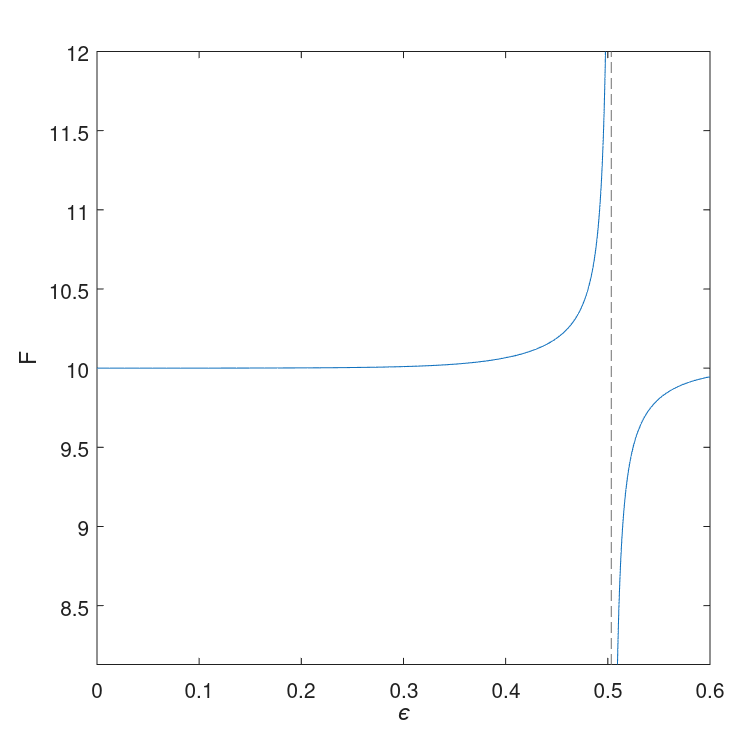
\includegraphics[width=0.48\textwidth]{figures/epsilon2F.png}
\caption{Graph of the function $f$.}
\label{fig:epsilon2F}
\end{figure}
In Figure~\ref{fig:epsilon2F} on the left we port the graph of $f$. We see that $\epsilon_0$, which correspond to the abscissa of the vertical asymptote, is slightly greater then $L/2$. In Figure~\ref{fig:plotu2p} we report the plot of $u_2$ and $p$ when $\epsilon=0.3$. In Figure~\ref{fig:bar} we report a picture of the bar when $\epsilon=0.493$. On the top there is the result obtained with a purely elastic bar while on the bottom the result predicted including the plastic behavior. The displacements of cross sections is magnified with a factor 7. The color represents the variable $p$.
\begin{figure}[p]
\centering
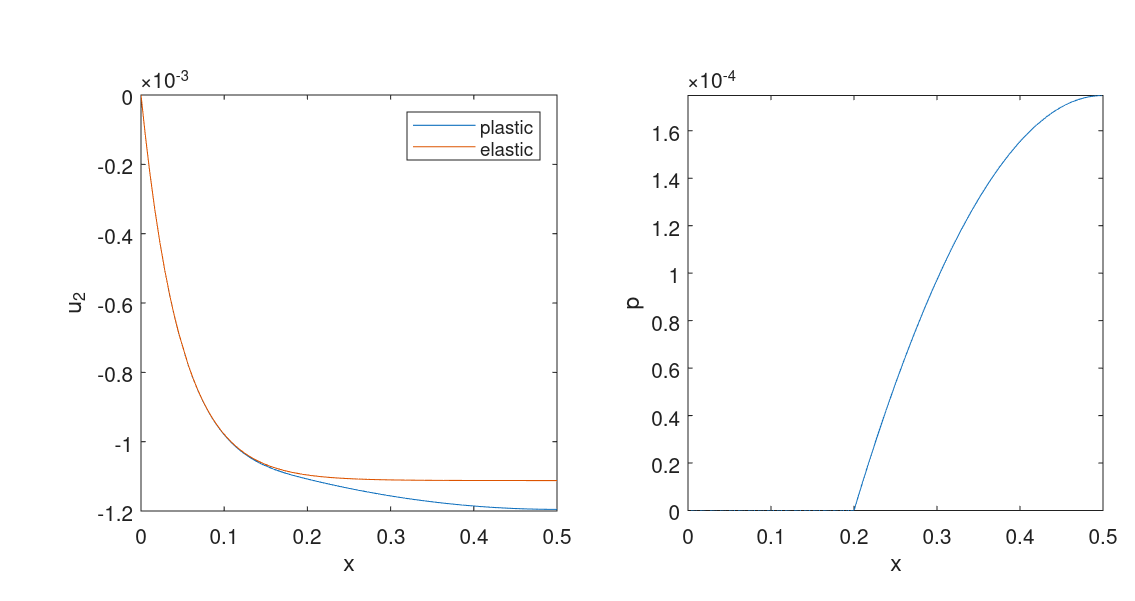
\includegraphics[width=\textwidth]{figures/plotu2p.png}
\caption{Plot of $u_2$ (left) and $p$ (right) for $\epsilon=0.3$.}
\label{fig:plotu2p}
\end{figure}
\begin{figure}[p]
\centering
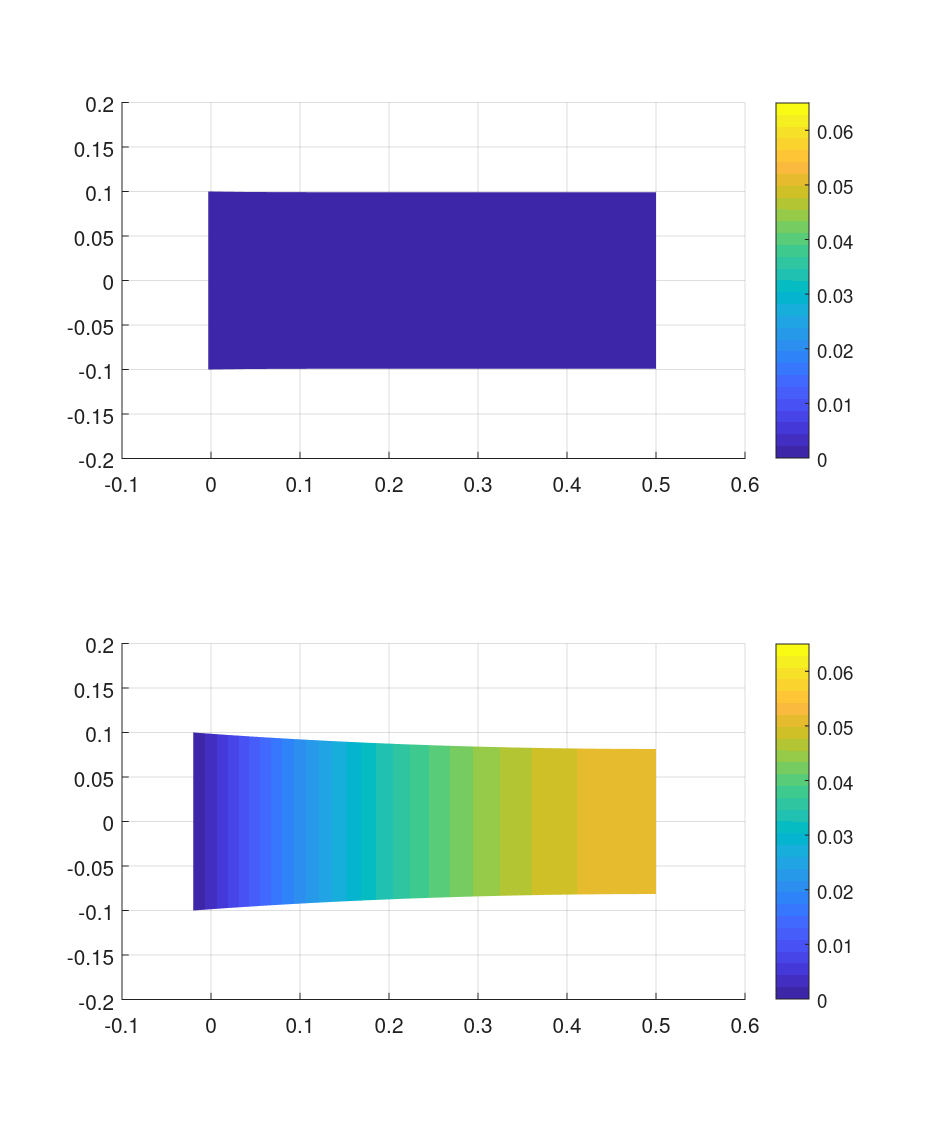
\includegraphics[width=\textwidth]{figures/bar.png}
\caption{Picture of the half $(0,L/2)$ of the bar when $\epsilon=0.493$. The bar on the bottom is plastic, the one on the top is purely elastic and subject to the same load. The transversal displacement is magnified with a factor 7. The color represents $p$.}
\label{fig:bar}
\end{figure}

\chapter{Large deformation model}

As we showed in the previous chapter, a small strain model of a bar is not able to predict necking. This leads us to consider a geometrically exact model that allows large deformations.

\section{Formulation}

\subsection{Motivation form the multidimensional kinematics}

Let $\Omega=(0,L)\times\Sigma\subset\mathbb{R}^d$ with $L>0$ and $\Sigma\subset\mathbb{R}^{d-1}$ the reference configuration of the cylindrical bar. The generic material point will be denoted as $(X,Y)\in\Omega$ with $X\in(0,L)$ and $Y\in\Sigma$. We consider deformations of the form
\[
(X,Y)\mapsto\begin{pmatrix}
\chi_1(X) \\
\chi_2(X)Y
\end{pmatrix}
\]
where $\chi_1\colon(0,L)\to\mathbb{R}$ satisfy $\chi_1'>0$ and $\chi_2\colon(0,L)\to(0,\infty)$. The corresponding deformation gradient is
\[
F=\begin{pmatrix}
\chi_1' & 0 \\
\chi_2'Y & \chi_2I
\end{pmatrix}.
\]
We define $\epsilon_1=\log\chi_1'$ and $\epsilon_2=\log\chi_2$. The plastic distortion is assumed to be of the form
\[
F_p=\begin{pmatrix}
P & 0 \\
0 & P^{-\frac{1}{d-1}}I
\end{pmatrix}
\]
where $P\colon(0,L)\to(0,\infty)$. This choice implies plastic incompressibility. We define $p=\log P$. The elastic distortion is then given by
\[
F_e=FF_p^{-1}=\begin{pmatrix}
\chi_1'P^{-1} & 0 \\
\chi_2'P^{-1}Y & \chi_2P^\frac{1}{d-1}I
\end{pmatrix}=
\begin{pmatrix}
E_1 & 0 \\
GY & E_2I
\end{pmatrix}.
\]
We define
\[
e_1=\log E_1=\epsilon_1-p\quad\text{and}\quad e_2=\log E_2=\epsilon_2+(d-1)^{-1}p.
\]
Now the spatial velocity gradient is given by
\[
L=\dot FF^{-1}=\begin{pmatrix}
\dot\epsilon_1 & 0 \\
\left(\frac{\dot\chi_2'}{\chi_1'}-\frac{\chi_2'}{\chi_1'}\dot\epsilon_2\right) & \dot\epsilon_2I
\end{pmatrix}
\]
and the plastic rate is
\[
L_p=\dot F_pF_p^{-1}=\begin{pmatrix}
\dot p & 0 \\
0 & -\frac{\dot p}{d-1}I
\end{pmatrix}.
\]
Then the elastic rate is
\[
L_e=\dot F_eF_e^{-1}=L-F_eL_pF_e^{-1}=\begin{pmatrix}
\dot e_1 & 0 \\
\left(\frac{\dot G}{E_1}-\frac{G}{E_1}\dot e_2\right)Y & \dot e_2I
\end{pmatrix}.
\]

\subsection{Kinematics}

Let $L>0$ the length of the cylindrical bar. The macroscopic configuration of the bar is described by $\chi_1\colon(0,L)\to\mathbb{R}$ with $\chi_1'>0$ and $\chi_2\colon(0,L)\to(0,\infty)$. Here $\chi_1$ describes the positions of the sections and $\chi_2$ is the transversal deformation factor of the sections. The configuration of the microscopic structure of the bar, that is the plastic distortion, is described by $P\colon(0,L)\to(0,\infty)$. We define the elastic distortions as $E_1=\chi_1'P^{-1}$, $E_2=\chi_2P^{\frac{1}{d-1}}$ and $G=\chi_2'P^{-1}$.

\subsection{Statics}

We assume that the internal power is given by
\[
\mathcal{W}=\int_0^L\left(\zeta\dot G+\sigma_1\dot E_1+\sigma_2\dot E_2\right)dX+\int_0^L\left(\tau\dot P+\kappa\dot P'\right)dX.
\]
Here $\zeta$ is the transversal elastic stress, $\sigma_1$ is the longitudinal elastic stress and $\sigma_2$ is the transversal elastic force while $\tau$ is the microscopic force and $\kappa$ the microscopic stress.
\begin{rmk}
In the small strain model of Chapter~\ref{chap:small-neck} we did not included the microscopic stress $\kappa$. However, we are now including it because we expect that in the large-strain regime, it is necessary to obtain an existence result in Sobolev spaces. This is suggested by the existence theorem for three-dimensional elastoplasticity at large strains presented in~\cite{mielke}.
\end{rmk} 
We notice that
\begin{gather*}
G^{-1}\dot G=(\chi_2')^{-1}\dot\chi_2'-P^{-1}\dot P \\
E_1^{-1}\dot E_1=(\chi_1')^{-1}\dot\chi_1'-P^{-1}\dot P \\
E_2^{-1}\dot E_2=\chi_2^{-1}\dot\chi_2+(d-1)^{-1}P^{-1}\dot P.
\end{gather*}
Then if we call $\tilde v_i$ the virtual rate of $\chi_i$ and $\tilde Q$ the virtual rate of $P$ we are let to consider the internal virtual power
\begin{multline*}
\tilde{\mathcal{W}}=\int_0^LG\zeta\left((\chi_2')^{-1}\tilde v_2'-P^{-1}\tilde Q\right)dX+\\
+\int_0^L\left[E_1\sigma_1\left((\chi_1')^{-1}\tilde v_1'-P^{-1}\tilde Q\right)+E_2\sigma_2\left(\chi_2^{-1}\tilde v_2+(d-1)^{-1}P^{-1}\tilde Q\right)\right]dX+\\
+\int_0^L\left[\tau\tilde Q+\kappa\tilde Q'\right]dX.
\end{multline*}
The external longitudinal and transversal forces distributed along the length of the bar and the external longitudinal and transversal forces acting on the extremities of the bar are included choosing the external power
\[
\tilde{\mathscr P}=\int_0^Lf\cdot\tilde vdx+h(L)\cdot\tilde v(L)-h(0)\cdot\tilde v(0).
\]
\begin{prop}
The local form of the equilibrium condition is
\begin{gather*}
(P^{-1}\sigma_1)'+f_1=0\quad\text{in $(0,L)$} \\
h_1(x)=P(x)^{-1}\sigma_1(x)\quad\text{for $x\in\{0,L\}$} \\
-P^{\frac{1}{d-1}}+(P^{-1}\zeta)'+f_2=0\quad\text{in $(0,L)$} \\
h_2(x)=P(x)^{-1}\zeta(x)\quad\text{for $x\in\{0,L\}$} \\
\chi_1'P^{-2}\sigma_1-(d-1)^{-1}\chi_2P^{\frac{1}{d-1}-1}\sigma_2+\chi_2'P^{-2}\zeta-\tau+\kappa'=0\quad\text{for $x\in\{0,L\}$} \\
\kappa(x)=0\quad\text{for $x\in\{0,L\}$}
\end{gather*}
\end{prop}
\begin{proof}
Rearranging the terms we have
\begin{multline*}
\tilde{\mathcal{W}}=\int_0^L\left[P^{-1}\sigma_1\tilde v_1'+P^{\frac{1}{d-1}}\sigma_2\tilde v_2+P^{-1}\zeta\tilde v_2'\right]dX+\\
+\int_0^L\left[\left(\tau-\chi_1'P^{-2}\sigma_1+(d-1)^{-1}\chi_2P^{\frac{1}{d-1}-1}\sigma_2-\chi_2'P^{-2}\zeta\right)\tilde Q+\kappa\tilde Q'\right]dX.
\end{multline*}
By integration by parts and application of the fundamental lemma of the calculus of variation we get the thesis.
\end{proof}

\subsection{Constitutive relations}

We choose a free energy for unit axial length of the form
\[
\psi=W(E_1,E_2,G)+H(P,P')
\]
where $W\colon(0,\infty)\times(0,\infty)\times\mathbb{R}\to\mathbb{R}$ is elastic free energy density and $H\colon(0,\infty)\times\mathbb{R}\to\mathbb{R}$ is the hardening free energy density. The plastic response is obtained by introducing a dissipation potential per unit axial length of the form
\[
\phi=R(P^{-1}\dot P)
\]
where $R\colon\mathbb{R}\to[0,\infty]$ satisfies $R(0)=0$. Consistently with that choice of $\psi$ and $\phi$ we impose the following constitutive relations
\begin{subequations}
\label{eqn:constitutive-neck-large}
\begin{gather}
\sigma_i=\dind{W}{E_i}\quad\text{and}\quad\zeta=\dind{W}{G} \\
\tau\in\dind{H}{P}+P^{-1}\partial R(P^{-1}\dot P)\quad\text{and}\quad\kappa=\dind{H}{P'}.
\end{gather}
\end{subequations}
\begin{prop}
The constitutive relations~\eqref{eqn:constitutive-neck-large} satisfy the dissipation inequality.
\end{prop}
\begin{proof}
Let $\tau=\dind{H}{P}+P^{-1}\xi$ with $\xi\in\partial R(\dot PP^{-1})$. Then dissipation per unit axial length is given by
\[
\zeta\dot G+\sigma_2\dot E_2+\sigma_2\dot E_2+\tau\dot P+\kappa\dot P'-\dot\psi=\xi P^{-1}\dot P.
\]
By definition of subdifferential we have $0=R(0)\ge R(P^{-1}\dot P)-\xi P^{-1}\dot P$ so that $\xi P^{-1}\dot P\ge R(P^{-1}\dot P)\ge0$. This implies that the dissipation is nonnegative.
\end{proof}

\part{Shear band localization in cohesive materials}

\chapter{Small deformation model}

\section{Formulation}

In this section we formulate the mechanical model. The description is made very quickly and we will expand it to give a better justification. In this section the emphasis is on the mechanical modeling, the correct functional setting will be investigated in the subsequent sections.

\subsection{Kinematics}

Let $\Omega\subset\mathbb{R}^d$ be the reference configuration of the body. The macroscopic displacement is a map $u\colon\Omega\to\mathbb{R}^d$. We set $E=\sym\grad u$ and $M=\grad^2 u$. We subdivide $\partial\Omega$ in two disjoint parts $\Gamma_D$ and $\Gamma_N$. On $\Gamma_D$ we impose the kinematical constrain $u=\overline u$. The configuration of the microscopic structure is described by the plastic distortion $H_p\colon\Omega\to\text{Lin}$. The skew symmetric part $W_p=\ske H_p$ describes the rotation of the microscopic structure and for simplicity we assume that it vanish. The symmetric part is the plastic strain $E_p=\sym H_p\colon\Omega\to\text{Sym}$ which describes the deformation of microscopic structure. We can regard $E_p$ as the elastically relaxed strain of the body so we define the elastic strain as $E_e=E-E_p$. The volumetric deformation of the microscopic structure is described by $\lambda_p=\tr E_p$ while the deviatoric deformation by $U_p=\dev E_p$. We call $M_p=\grad U_p$ and we set $\mathbb{U}_p=(U_p,l\,M_p)\in\text{DevPla}$ where $l>0$ is an internal length scale. Here $\text{DevPla}=\text{Sym}\otimes(\text{Sym}\otimes\mathbb{R})$ is the vector space of the deviatoric plastic strains and their gradients. In what follows we will denote with $\circ$ the natural scalar product on $\text{DevPla}$. We assume that the material is not dilatant (this is a simplification and should be generalized to describe the dilatant behavior observed in most materials exhibiting a pressure dependent yield strength) so we add the constrain $\lambda_p=0$. To impose this constrain we add the Lagrange multiplier $p\colon\Omega\to\mathbb{R}$ with the meaning of a plastic pressure. The constrain can be written in weak form as
\[
\int_\Omega\lambda_p\tilde qdx=0\quad\text{for all $\tilde q\colon\Omega\to\mathbb{R}$}.
\]

\subsection{Statics}

We denote with $\tilde v$, $\tilde L_p$ $\tilde V_p$ and $\tilde\mu_p$ the virtual rates of $u$, $E_p$, $U_p$ and $\lambda_p$ respectively. The virtual rate of $E_e$ is $\tilde L_e=\grad\tilde v-\tilde L_p$ where $\tilde L=\grad\tilde v$. Due to the presence of the Dirichlet condition we require that $\tilde v$ vanish on $\Gamma_D$. Instead we do not require that $\tilde\mu_p=0$ because the constrain $\lambda_p=0$ is imposed by mean of the Lagrange multiplier $p$. To describe the coupling between the macroscopic deformation $u$ and the microscopic configuration $E_p$ we choose an internal virtual power of the form
\[
\begin{split}
\tilde{\mathcal{W}}&=\int_\Omega\left(T:\tilde L+K\threedots\grad^2\tilde v\right)dx+\int_\Omega T_e:\tilde L_edx+\int_\Omega\left(T_p:\tilde V_p+K_p\threedots\grad\tilde V_p\right)dx.
\end{split}
\]
The first integral is related to the macroscopic response. Here $T\in\text{Sym}$ is the macrostress and $K\in\text{Lin}\otimes\mathbb{R}$ is the macrohyperstress. The presence of the second order of $\tilde v$ is due to the need of a sufficient regularization in view of the existence theorem. The second integral describe the coupling between the macroscopic and the microscopic response and $T_e\in\text{Sym}$ is the elastic stress. The third integral is associated with the microscopic response. Here $T_p\in\text{DevSym}$ is the microforce and $K_p\in\text{DevSym}\otimes\mathbb{R}$ is the microstress. In Figure~\ref{fig:rheological} we
report a picture that represents schematically the meaning of the internal virtual power
that we have chosen. We define $\tilde{\mathbb{V}}_p=(\tilde V_p,l\grad\tilde V_p)$ and $\mathbb{T}_p=(T_p,l^{-1}K_p)$ so that
\[
T_p:\tilde V_p+K_p\threedots\grad\tilde V_p=\mathbb{T}_p\circ\tilde{\mathbb{V}}_p.
\]
\begin{figure}
\centering
\begin{tikzpicture}[thick, scale=1]
% Ingressi laterali
\draw (-0.5,0) -- (0,0);
\draw (4,0) -- (3.5,0);

% Connessioni verticali
\draw (0,0) -- (0,1) -- (1.25,1);
\draw (0,0) -- (0,-1) -- (0.5,-1);
\draw (3.5,0) -- (3.5,-1) -- (3,-1);
\draw (3.5,0) -- (3.5,1) -- (2.25,1);

% Ramo Superiore: Blocco T
\draw (1.25,0.75) rectangle (2.25,1.25);
\node[anchor=south] at (1.75,1.25) {$T$};

% Ramo Inferiore: Molla Te (disegnata segmento per segmento)
\draw (0.5,-1) -- (0.571,-0.75) -- (0.714,-1.25) -- (0.857,-0.75) -- (1,-1.25) -- (1.143,-0.75) -- (1.286,-1.25) -- (1.429,-0.75) -- (1.5,-1);
\node[anchor=north] at (1,-1.25) {$T_e$};
\draw (1.5,-1) -- (2.5,-1);

% Ramo Inferiore: Smorzatore Tp
\draw (2.5,-1.125) -- (2.5,-0.875); % Pistone
\draw (2,-0.75) -- (3,-0.75) -- (3,-1.25) -- (2,-1.25); % Cilindro
\node[anchor=north] at (2.5,-1.25) {$T_p$};
\end{tikzpicture}
\caption{Rheological model describing the choice of the internal virtual power $\tilde{\mathscr W}$. The
box in upper branch represents the (generic) macroscopic response. In the lower branch,
the spring represents the elastic response and the piston represents the microscopic response. We
notice that the microscopic response besides the usual dissipative plastic microforce force can include conservative microforces to model hardening. A more detailed discussion on constitutive relations is in Section~\ref{subsec:constitutive}.}
\label{fig:rheological}
\end{figure}
The action of the plastic pressure is obtained by considering the reaction virtual power
\[
\tilde{\mathscr{R}}=-\int_\Omega p\tilde\mu_pdx.
\]
We notice that this power vanish on virtual rates that satisfy the constrain that is $\tilde\mu_p=0$. The external actions of the volume force $f$ on $\Omega$ and the traction $h$ on $\Gamma_N$ are included choosing the external virtual power
\[
\tilde{\mathcal{P}}=\int_\Omega f\cdot\tilde vdx+\int_{\Gamma_N}h\cdot\tilde vdx.
\]
For simplicity we assume that no external torque is applied to the body and that there is no external action on the microscopic configuration. These external actions could be added to describe more accurately the boundary conditions imposed on the body.
\begin{lemma}
The local form of the equilibrium condition is
\begin{align*}
&\diver(T+T_e-\diver K)+f=0\quad\text{in $\Omega$} \\
&(T+T_e-\diver K)n-\diver_P((Kn)P)=h\quad\text{in $\Gamma_N\cap\partial^{d-1}\Omega$} \\
&\{\!\!\{(Kn)\tau\}\!\!\}=0\quad\text{in $\partial^{d-2}\Omega$} \\
&-\dev T_e+T_p-\diver K_p=0\quad\text{in $\Omega$} \\
&p=-\frac{1}{d}\tr T_e\quad\text{in $\Omega$} \\
&K_p n=0\quad\text{in $\partial^{d-1}\Omega$}.
\end{align*}
\end{lemma}
\begin{proof}
By integration by parts we can write
\begin{multline*}
\int_\Omega\left(T:\grad\tilde v+K\threedots\grad^2\tilde v\right)dx=\\
=-\int_\Omega\diver(T-\diver K)\cdot\tilde vdx+\int_{\partial^{d-1}\Omega}\left[(T-\diver K)n\cdot\tilde v+Kn:\grad\tilde v\right]dx.
\end{multline*}
Now denoting with $P=I-n\otimes n$ the projector on $\partial^{d-1}\Omega$ we have
\[
Kn:\grad\tilde v=Kn:\left(\dind{\tilde v}{n}\otimes n+\grad_P\tilde v\right)=(Kn)n\cdot\dind{\tilde v}{n}+Kn:\grad_P\tilde v
\]
and
\[
Kn:\grad_P\tilde v=(Kn)P:\grad_P\tilde v=\diver_P(P(Kn)^T\tilde v)-\diver_P((Kn)P)\cdot\tilde v.
\]
But by integration by parts
\[
\int_{\partial^{d-1}\Omega}\diver_P(P(Kn)^T\tilde v)dx=\int_{\partial^{d-2}\Omega}\{\!\!\{P(Kn)^T\tilde v\cdot\tau\}\!\!\}dx=\int_{\partial^{d-2}\Omega}\{\!\!\{(Kn)\tau\}\!\!\}\cdot\tilde vdx.
\]
Here $\{\!\!\{\cdot\}\!\!\}$ denotes sum of its argument evaluated on both sides of $\partial^{d-2}\Omega$ and $\tau$ denotes the unit normal vector to $\partial^{d-2}\Omega$ and outer tangent to $\partial^{d-1}\Omega$. We have obtained
\begin{multline*}
\int_\Omega\left(T:\grad\tilde v+K\threedots\grad^2\tilde v\right)dx=\\
=-\int_\Omega\diver(T-\diver K)\cdot\tilde vdx+\int_{\partial^{d-1}\Omega}\left[(T-\diver K)n-\diver_P((Kn)P)\right]\cdot\tilde vdx+\\
+\int_{\partial^{d-1}\Omega}(Kn)n\cdot\dind{\tilde v}{n}dx+\int_{\partial^{d-2}\Omega}\{\!\!\{(Kn)\tau\}\!\!\}\cdot\tilde vdx.
\end{multline*}
Moreover the remaining terms of the virtual power can be written as
\begin{multline*}
-\int_\Omega\diver T_e:\tilde vdx+\int_{\partial^{d-1}\Omega}T_en\cdot\tilde vdx+\int_\Omega(T_p-\dev T_e-\diver K_p):\tilde V_pdx+\\
+\int_{\partial^{d-1}\Omega}K_pn:\tilde V_pdx-\int_\Omega\frac{1}{d}\tr T_e\tilde\mu dx.
\end{multline*}
Now the results follows from the fundamental lemma of the calculus of variations.
\end{proof}

\subsection{Constitutive relations}
\label{subsec:constitutive}

We assume a constitutive relation for the free energy density of the form
\[
\psi=\frac{1}{2}\mathfrak{C}E_e:E_e+\frac{1}{2}\mathfrak{A}M\threedots M+\frac{1}{2}\mathfrak{B}\mathbb{U}_p\circ\mathbb{U}_p.
\]
with $\mathfrak{C}$, $\mathfrak{A}$ and $\mathfrak{B}$ a symmetric and positive definite linear operators on $\text{Sym}$, $\text{Lin}\otimes\mathbb{R}$ and $\text{DevPla}$ respectively. Moreover we choose a dissipation potential density of the form
\[
\phi=\frac{1}{2}\mathfrak{D}\dot E:\dot E+\frac{1}{2}\mathfrak{E}\dot M\threedots\dot M+\frac{1}{2}\mathfrak{F}\dot{\mathbb{U}}_p\circ\dot{\mathbb{U}}_p+Y(p)G(\dot U_p).
\]
Here $\mathfrak{D}$, $\mathfrak{E}$, $\mathfrak{F}$ are symmetric and positive definite linear operators on $\text{Sym}$, $\text{Lin}\otimes\mathbb{R}$ and $\text{DevPla}$ respectively. Moreover $G\colon\text{DevSym}\to[0,\infty]$ is the convex and subdifferentiable plastic dissipation potential satisfying $G(0)=0$ and $Y\colon\mathbb{R}\to[0,\infty)$ is the pressure dependent yield strength.
Consistently with these choices of the free energy density and of the dissipation potential density we impose the following constitutive relations. The macroscopic response is described by
\[
T=\mathfrak{D}\dot E\quad\text{and}\quad K=\mathfrak{A}M+\mathfrak{E}\dot M.
\]
with $\mathfrak{D}$ and $\mathfrak{E}$ symmetric and positive definite linear operators on $\text{Sym}$ and $\text{Lin}\otimes\mathbb{R}$ respectively. The elastic response is given by
\[
T_e=\mathfrak{C}E_e
\]
and the viscoplastic response by
\[
\mathbb{T}_p\in\mathfrak{B}\mathbb{U}_p+\mathfrak{F}\dot{\mathbb{U}}_p+Y(p)\partial_{\dot U_p}G(\dot U_p)
\]
where $\mathfrak{F}$ is a symmetric positive definite tensor on $\text{DevPla}$, $G\colon\text{DevSym}\to\mathbb{R}$ is the plastic dissipation potential satisfying $\partial_{\dot U_p}G(\dot U_p):\dot U_p\ge0$ and $Y\colon\mathbb{R}\to[0,\infty)$ is the pressure dependent yield strength.
\begin{rmk}
In the above expression we are viewing $Y(p)\partial_{\dot U_p}G(\dot U_p)\in\text{DevSym}$ as an element of $\text{DevPla}$ by considering $\text{DevSym}$ as a subspace of $\text{DevPla}$.
\end{rmk}
%\begin{lemma}
%The constitutive relations satisfy the dissipation inequality.
%\end{lemma}
%\begin{proof}
%The rate of the free energy per unit volume is
%\[
%\dot\psi=\mathfrak{C}E_e:\dot E_e+\mathfrak{A}M\threedots\grad^2\dot u+\mathfrak{B}\mathbb{U}_p\circ\dot{\mathbb{U}}_p
%\]
%We notice that
%\[
%T_p:\dot U_p+K_p\threedots\grad\dot U_p=\mathbb{T}_p\circ\dot{\mathbb{U}}_p
%\]
%Then the internal power per unit volume is
%\begin{multline*}
%\mathfrak{D}\dot E:\dot E+\mathfrak{A}M\threedots\grad^2\dot u+\mathfrak{E}\grad^2\dot u\threedots\grad^2\dot u+\mathfrak{C}E_e:\dot E_e+\\
%+\mathfrak{B}\mathbb{U}_p\circ\dot{\mathbb{U}}_p+\mathfrak{F}\dot{\mathbb{U}}_p\circ\dot{\mathbb{U}}_p+Y(p)\partial_{\dot U_p}G(\dot U_p):\dot{U}_p.
%\end{multline*}
%Taking the difference we find that the dissipation rate per unit volume is
%\[
%\mathfrak{D}\dot E:\dot E+\mathfrak{F}\dot{\mathbb{U}}_p\circ\dot{\mathbb{U}}_p+Y(p)\partial_{\dot U_p}G(\dot U_p):\dot{U}_p\ge0.
%\]
%This concludes the proof.
%\end{proof}

\subsection{Refinements of the model}

To include the dilatancy in the model we could do the following. We put the unilateral constrain $\lambda_p\ge F(U_p)$, meaning that when the microscopic structure suffer shear distortions it must suffer also an expansion. This constrain is still imposed through the Lagrange multiplier $p$ representing the microscopic pressure. To make the expansion irreversible (once the microscopic structure expanded it can not be compacted again) we add a microscopic force $\xi$ conjugate to $\tilde\mu_p$ in the internal virtual power and in the dissipation potential density we add $\iota_{[0,\infty)}(\dot\xi)$. In this way $\xi$ opposes to the compaction of the microscopic structure.

%\subsection{Refinements of the model}
%
%Until now the model is a reformulation of Drucker--Prager model as is not able to describe compaction but only dilatancy. We could refine this aspect trying to reproduce the behavior of Cam-Clay model. We could add a field $\delta_p$ representing the volumetric deformation of the grains. Then the quantity representing the amount of void would be represented by $\lambda_p-\delta_p$. In this case the constrain is $\dot\lambda_p-\dot\delta_p=F(\lambda_p,\delta_p,\dot U_p)$. Now $p$ would be power conjugate to $\tilde{\dot\lambda}_p-\tilde{\dot\delta}_p$. An additional microscopic force $\tau_p$ would appear power conjugate to $\tilde{\dot\delta}_p$. We get the additional microforce balance
%\[
%p+\tau_p=0.
%\]
%The constitutive relation could be $\tau_p=\partial\gamma_p(\dot\delta_p)$ to describe a dissipative effect.
%
%A further refinement could be the addition of plastic spin $W_p\in\text{Skew}$. We notice that since the second gradient elasticity that we have introduced is independent of the plastic behavior\footnote{Because $K$ is conjugate to $\tilde{\dot M}$ and not to $\tilde{\dot M}_e$ with $M_e=\grad H_e$ and $H_e=H-H_p$)} (this was done for mathematical reasons, since we needed compactness to apply Schauder theorem) then the rotational force would come only from the plastic behavior in the sense that: the macroscopic stress only exert a symmetric microforce that in principle only change $E_p$ but the plastic response can cause also a nonsymmetric zero microforce so that $W_p$ can became nonzero.

\section{Mathematical analysis}

In what follows we write simply $U$ and $\lambda$ in place of $U_p$ and $\lambda_p$ respectively. Moreover for simplicity we assume $\Gamma_D=\partial\Omega$ and $\overline{u}=0$ since the extension to the general case in trivial.

\subsection{Hypotheses}
\label{subsec:hypotheses}

To get the global existence result we assume the following hypotheses.
\begin{itemize}
\item[(S)]
\begin{itemize}[noitemsep]
\item[(a)] $\Omega\subset\mathbb{R}^d$ with $d\in\{2,3\}$ is open, bounded and Lipschitz
\item[(b)] $\Gamma_D$ and $\Gamma_N$ are relatively open disjoint subsets of $\partial\Omega$
\end{itemize}
\item[(Y)]
\begin{itemize}[noitemsep]
\item[(a)] $Y\in C^{0,1}(\mathbb{R},[0,\infty))$
\end{itemize}
\item[(G)]
\begin{itemize}[noitemsep]
\item[(a)] $G\in C^{1,1}(\text{DevSym},\mathbb{R})$ is convex
\item[(b)] $\partial G\in L^\infty(\text{DevSym},\text{DevPla})$
\item[(c)] $\partial G(\dot U):\dot U\ge0$ for all $\dot U\in\text{DevSym}$
\end{itemize}
\item[(L)]
\begin{itemize}[noitemsep]
\item[(a)] $f\in C^1([0,T],L^2(\Omega)^d)$
\item[(b)] $h\in C^1([0,T],L^2(\Gamma_N)^d)$
\end{itemize}
\item[(E)]
\begin{itemize}[noitemsep]
\item[(a)] $\mathfrak{C}$ and $\mathfrak{D}$ are in $\text{Sym}\otimes\text{Sym}$, $\mathfrak{B}$ and $\mathfrak{F}$ are in $\text{DevPla}\otimes\text{DevPla}$, $\mathfrak{A}$ and $\mathfrak{E}$ are in $(\text{Lin}\otimes\mathbb{R})\otimes(\text{Lin}\otimes\mathbb{R})$
\item[(b)] there exist $\gamma>0$ and $\delta>0$ such that $\mathfrak{C}E:E\ge\gamma|E|^2$ and $\mathfrak{D}E:E\ge\delta|E|^2$ for all $E\in\text{Sym}$, there exist $\beta>0$ and $\phi$ such that $\mathfrak{B}\mathbb{U}\circ\mathbb{U}\ge\beta|\mathbb{U}|^2$ and $\mathfrak{F}\mathbb{U}\circ\mathbb{U}\ge\phi|\mathbb{U}|^2$, there exists $\alpha>0$ and $\epsilon>0$ such that $\mathfrak{A}M\threedots M\ge\alpha|\sym M|^2$ and $\mathfrak{E}M\threedots M\ge\epsilon|\sym M|^2$ for all $M\in\text{Lin}\otimes\mathbb{R}$ where $\sym$ denote the symmetrization of the first two indices
\end{itemize}
\end{itemize}

\subsection{Function spaces}

We now introduce the function spaces that we use to formulate the problem. Let
\[
\mathscr{Z}=\left\{y=(u,U,\lambda)\middle|\substack{\text{$u\in H^2(\Omega)^d$ and $u=0$ on $\Gamma_D$}\\U\in H^1(\Omega,\text{DevSym})\\\lambda\in L^2(\Omega)}\right\}\quad\text{and}\quad\mathscr{Q}=\left\{p\in L^2(\Omega)\right\}.
\]
The rates of $y=(u,U,\lambda)\in\mathscr{Z}$ will be denoted by $\dot y=(\dot u,\dot U,\dot\lambda)\in\mathscr{Z}$. The variations of $\dot y=(\dot u,\dot\xi,\dot\lambda)\in\mathscr{Z}$ and $p\in\mathscr{Q}$ will be denoted as $z=(v,V,\mu)\in\mathscr{Z}$ and $q\in\mathscr{Q}$. The test functions will be denoted as $\tilde z=(\tilde v,\tilde V,\tilde\mu)$.

\subsection{Formulation of the problem}

We define $\mathcal{F}\colon\mathscr{Z}\times\mathscr{Q}\times\mathscr{Z}\times[0,T]\to\mathscr{Z}'\times\mathscr{Q}'$ by
\[
\begin{split}
\dual{\mathcal{F}(\dot y,p,y,t),(\tilde z,\tilde q)}=\int_\Omega\mathfrak{C}\left(Eu-U-\frac{\lambda}{d}I\right):\left(E\tilde v-\tilde V-\frac{\tilde\mu}{d}I\right)dx+\\
+\int_\Omega(\mathfrak{A}\grad^2 u+\mathfrak{E}\grad^2\dot u)\threedots\grad^2\tilde vdx+\int_\Omega\mathfrak{D} E\dot u:E\tilde vdx+\\
+\int_\Omega\left[(\mathfrak{B}\mathbb{U}+\mathfrak{F}\dot{\mathbb{U}})\circ\tilde{\mathbb{V}}+Y(p)\partial G(\dot U):\tilde V\right]dx-\\
-\int_\Omega p\tilde\mu dx-\int_\Omega\lambda\tilde qdx-\\
-\int_\Omega f(t)\cdot\tilde vdx-\int_{\Gamma_N}h(t)\cdot\tilde vdx.
\end{split}
\]
\begin{lemma}
\label{lemma:F-well}
The map $\mathcal{F}$ is well defined.
\end{lemma}
\begin{proof}
The linear terms are trivially well defined so we need to check only
\begin{equation}
\label{eqn:nonlinear-terms-F}
\int_{\Omega}Y(p)\partial G(\dot U):\tilde Vdx.
\end{equation}
But
\[
\int_{\Omega}|Y(p)||\partial G(\dot{\mathbb{U}})||\tilde{\mathbb V}|dx\le\norm{\partial G}_\infty\int_{\Omega}(Y(0)+\text{Lip}(Y)|p|)|\tilde{\mathbb V}|dx\lesssim(1+\norm{p}_2)\norm{\tilde V}_{1,2}.
\]
This concludes the proof.
\end{proof}
Now we can formulate the evolution problem as follows.
\begin{prb}
\label{prb:problem}
Find $y\in H^1((0,T),\mathscr{Z})$ and $p\in L^2([0,T],\mathscr{Q})$ such that $y(0)=0$ and
\[
\mathcal{F}(\dot y(t),p(t),y(t),t)=0
\]
for almost every $t\in(0,T)$.
\end{prb}

\subsection{Global existence}
\label{subsec:existence}

This section is devoted to prove the following existence of a global in time solution to Problem~\ref{prb:problem}.
\begin{thm}
\label{thm:global-existence}
Assume the hypotheses of Section~\ref{subsec:hypotheses}. Then there exists $y\in H^1((0,T),\mathscr{Z})$ and $p\in C^0([0,T],\mathscr{Q})$ solution to Problem~\ref{prb:problem}.
\end{thm}
The proof is based on the Rothe method so we first prove the existence to a discrete in time version of the problem and then we pass to the vanishing time step limit. 

\subsubsection*{Existence of the discrete in time solution}

Let $N\in\mathbb{N}$. We define $\tau_N=N^{-1}T$ and $t_n^N=n\tau_N$ for $n\in\{0,\dots,N\}$. We consider the discrete in time version of Problem~\ref{prb:problem}.
\begin{prb}[Discrete problem]
\label{prb:discrete-problem}
Let $y_0^N=0\in\mathscr{Z}$. Find $y_n^N\in\mathscr{Z}$ and $p_n^N\in\mathscr{Q}$ for $n\in\{1,\dots,N\}$ such that
\begin{equation}
\label{eqn:incremental-step-n}
\mathcal{F}\left(\frac{y_n^N-y_{n-1}^N}{\tau_N},p_n^N,y_n^N,t_n^N\right)=0
\end{equation}
for all $n\in\{1,\dots,N\}$.
\end{prb}
We first prove the existence of a solution to Problem~\ref{prb:discrete-problem}. Reasoning by induction we reduce to find $y_n^N\in\mathscr{Z}$ and $p_n^N\in\mathscr{Q}$ that satisfy~\eqref{eqn:incremental-step-n} given $y_{n-1}^N\in\mathscr{Z}$. We immediately observe that in view of the constrain $\lambda_n^N=0$ for all $n$. To simplify the notation we call $y=y_{n-1}^N$, $\dot y=\tau^{-1}(y^N_n-y^N_{n-1})$ and $t=t_n^N$. Then $y_n^N=y+\tau\dot y$. It is enough to prove that there exists $\dot y\in\mathscr{Z}$ and $p\in Q$ such that
\begin{equation}
\label{eqn:time-step-abstract}
\mathcal{F}(\dot y,p,y+h\dot y,t)=0.
\end{equation}
We define the operator $\mathcal{A}\colon\mathscr Q\times\mathscr{Z}\to\mathscr{Z}'$ by
\[
\begin{split}
\dual{\mathcal{A}(p,\dot y),\tilde z}=\int_\Omega\tau\mathfrak{C}\left(E\dot u-\dot U-\frac{\dot\lambda}{d}I\right):\left(E\tilde v-\tilde V-\frac{\tilde\mu}{d}I\right)dx+\int_\Omega\mathfrak{D}E\dot u:E\tilde vdx+\\
+\int_\Omega(\mathfrak{E}+\tau \mathfrak{A})\grad^2\dot u\threedots\grad^2\tilde vdx+\int_\Omega\left[(\mathfrak{F}+\tau\mathfrak{B})\mathbb{\dot U}\circ\tilde{\mathbb{V}}+Y(p)\partial G(\dot U):\tilde V\right]dx
\end{split}
\]
the linear operator $\mathcal{B}\colon\mathscr{Q}\to\mathscr{Z}'$ by
\[
\dual{\mathcal{B}p,\tilde z}=-\int_\Omega p\tilde\mu dx
\]
and the operator $\mathcal{C}\colon\mathscr{Z}\to\mathscr{Q}'$ by
\[
\dual{\mathcal{C}(\dot y),\tilde q}=\int_\Omega(\lambda+\tau\dot\lambda)\tilde qdx=0.
\]
Moreover we introduce the linear form $l\in\mathscr{Z}'$
\[
\begin{split}
\dual{l,\tilde z}=\int_\Omega f(t)\cdot\tilde vdx+\int_{\Gamma_N}h(t)\cdot\tilde vdx-\\
-\int_\Omega\mathfrak{C}\left(Eu-U-\frac{\lambda}{d}I\right):\left(E\tilde v-\tilde V-\frac{\tilde\mu}{d}I\right)dx-\\
-\int_\Omega\mathfrak{A}\grad^2 u\threedots\grad^2\tilde vdx-\int_\Omega\mathfrak{B}\mathbb{U}\circ\tilde{\mathbb{V}}dx.
\end{split}
\]
Now equation~\eqref{eqn:time-step-abstract} can be written as
\begin{equation*}
\begin{cases}
\mathscr{A}(p,\dot y)+Bp=l(t) \\
\mathscr{C}(\dot y)=0.
\end{cases}
\end{equation*}
We have already noticed that $\lambda=0$ and $\dot\lambda=0$. We call
\[
\mathscr{N}=\left\{\dot y=(\dot u,\dot U,0)\;\middle|\;\substack{\text{$\dot u\in H^2(\Omega)^d$ and $\dot u=0$ on $\Gamma_D$}\\\dot U\in H^1(\Omega,\text{DevSym})}\right\}.
\]
Now we study the first equation in~\eqref{eqn:time-step-abstract}. We first study the solvability of that equation in $\dot y\in\mathscr{N}$ given $p\in\mathscr{Q}$. If we test the first equation with $\tilde{z}\in\mathscr{N}$ we get
\[
\dual{\mathcal{A}(p,\dot y),\tilde{z}}=\dual{l,\tilde{z}}\quad\text{for all $\tilde{z}\in\mathscr{N}$}.
\]
Now we define the space
\[
\mathscr{X}=\left\{\xi=(\dot u,\dot U)\;\middle|\;\substack{\text{$\dot u\in H^2(\Omega)^d$ and $\dot u=0$ on $\Gamma_D$}\\\dot U\in H^1(\Omega,\text{DevSym})}\right\}
\]
and we can consider the natural bijection $\mathcal{J}$ from $\mathscr{X}$ to $\mathscr{N}$. In particular if $\xi=(\dot u,\dot U)$ we define
\[
\mathcal{J}(\xi)=(\dot u,\dot U,0).
\]
Now we introduce the operator $\mathcal{T}_p$ from $\mathscr{X}$ to $\mathscr{X}'$ as follows. Given $\xi=(\dot u,\dot U)$ and $\tilde{\zeta}=(\tilde{v},\tilde{V})$ in $\mathscr{X}$ we set
\[
\begin{split}
\dual{\mathcal{T}_p(\xi),\tilde{\zeta}}=\dual{\mathscr{A}(p,\mathscr{J}(\xi)),\mathscr{J}(\tilde\zeta)}=\int_\Omega\tau\mathfrak{C}\left(E\dot u-\dot U\right):\left(E\tilde v-\tilde V\right)dx+\int_\Omega\mathfrak{D}E\dot u:E\tilde vdx+\\
+\int_\Omega(\mathfrak{E}+\tau \mathfrak{A})\grad^2\dot u\threedots\grad^2\tilde vdx+\int_\Omega\left[(\mathfrak{F}+\tau\mathfrak{B})\mathbb{\dot U}\circ\tilde{\mathbb{V}}+Y(p)\partial G(\dot U):\tilde V\right]dx.
\end{split}
\]
Now for each $p\in\mathscr{Q}$ we are reduced to find $\xi\in\mathscr{X}$ such that
\begin{equation}
\label{eqn:T}
\dual{\mathcal{T}_p(\xi),\tilde\zeta}=\dual{l,\mathcal{J}(\tilde\zeta)}\quad\text{for all $\tilde\zeta\in\mathscr{X}$}.
\end{equation}
We want to apply the Browder--Minty theorem (Theorem~\ref{thm:browder-minty}). We need to establish the boundedness, continuity, coercivity and monotonicity of $\mathcal{T}_p$. This done in the following lemmas.
\begin{lemma}
The operator $\mathcal{T}_p\colon\mathscr{X}\to\mathscr{X}'$ is bounded and continuous.
\end{lemma}
\begin{proof}
We have
\[
\begin{split}
|\dual{\mathcal{T}_p(\xi),\tilde{\zeta}}|\lesssim\left(\norm{E\dot u}_2+\norm{\dot U}_2\right)\left(\norm{E\tilde v}_2+\norm{\tilde V}_2\right)+\\
+\norm{\grad^2\dot u}_2\norm{\grad^2\tilde v}_2+\norm{\mathbb{\dot U}}_2\norm{\tilde{\mathbb{V}}}_2+(1+\norm{p}_2)\norm{\tilde{\mathbb{V}}}_2.
\end{split}
\]
and this proves that $\mathcal{T}_p$ is bounded. Now it is enough to prove the continuity of the nonlinear term only. Let $\xi_n\to\xi$ in $\mathscr{X}$. Then $\dot{\mathbb{U}}_n\to\dot{\mathbb{U}}$ in $L^2$. We have
\[
\left|\int_\Omega Y(p)(\partial G(\dot{\mathbb{U}}_n)-\partial G(\dot{\mathbb{U}}))\circ\tilde{\mathbb{V}}dx\right|\le\norm{Y(p)(\partial G(\dot{\mathbb{U}}_n)-\partial G(\dot{\mathbb{U}}))}_2\norm{\tilde{\mathbb{V}}}_2
\]
and
\[
\norm{Y(p)(\partial G(\dot{\mathbb{U}}_n)-\partial G(\dot{\mathbb{U}}))}_2^2=\int_\Omega Y(p)^2(\partial G(\dot{\mathbb{U}}_n)-\partial G(\dot{\mathbb{U}}))^2dx\to0.
\]
Indeed for every subsequence there exists a further subsequence such that $\dot{\mathbb{U}}_n\to\dot{\mathbb{U}}$ in $L^2$ and we can apply the dominated convergence theorem to pass to the limit.
\end{proof}
\begin{lemma}
\label{lemma:coercivity-T}
The operator $\mathcal{T}_p\colon\mathscr{X}\to\mathscr{X}'$ is coercive uniformly in $p$.
\end{lemma}
\begin{proof}
For any $\xi\in\mathscr{X}$ we have
\[
\begin{split}
\dual{\mathcal{T}_p(\xi),\xi}=\int_\Omega\tau\mathfrak{C}\left(E\dot u-\dot U\right):\left(E\dot u-\dot U\right)dx+\int_\Omega\mathfrak{D}E\dot u:E\dot udx+\\
+\int_\Omega(\mathfrak{E}+\tau \mathfrak{A})\grad^2\dot u\threedots\grad^2\dot udx+\int_\Omega\left[(\mathfrak{F}+\tau\mathfrak{B})\mathbb{\dot U}\circ\mathbb{\dot U}+Y(p)\partial G(\dot U)\circ\dot U\right]dx.
\end{split}
\]
Using the hypotheses (E, b) and (G, b) and using that $\dot U:I=0$ since $\dot U\in\text{Dev}$ we have
\[
\dual{\mathcal{T}_p(\xi),\xi}\ge\tau\gamma\left\lVert E\dot u-\dot U\right\rVert_2^2+\tau\alpha\norm{\grad E\dot u}_2^2+(\phi+\tau\beta)\norm{\dot{\mathbb{U}}}_2^2.
\]
By the Young inequality
\[
\left\lVert E\dot u-\dot U\right\rVert_2^2\ge(1-\theta)\norm{E\dot u}_2^2+\left(1-\frac{1}{\theta}\right)\norm{\dot U}_2^2
\]
for any $\theta>0$. Then
\[
\begin{split}
\dual{\mathcal{T}_p(\xi),\xi}\ge(1-\theta)\tau\gamma\norm{E\dot u}_2^2+\tau\alpha\norm{\grad E\dot u}_2^2+\\
+\left(1-\frac{1}{\theta}\right)\tau\gamma\norm{\dot U}_2^2+(\phi+\tau\beta)\norm{\dot{\mathbb{U}}}_2^2.
\end{split}
\]
We choose $\theta<1$ sufficiently close to 1 such there exists a constant $C_1>0$ with the property that
\[
\left(1-\frac{1}{\theta}\right)\tau\gamma\norm{\dot U}_2^2+(\phi+\tau\beta)\norm{\dot{\mathbb{U}}}_2^2\ge C_1\norm{\dot{\mathbb{U}}}_2^2\ge C_2\norm{\dot U}_{1,2}^2.
\]
The thesis follows by application of Korn inequality.
\end{proof}
%\begin{lemma}
%\label{lemma:monotone-T}
%We can write $\mathcal{T}_p=\mathcal{R}_p+\mathcal{Q}$ with $\mathcal{R}_p\colon\mathscr{X}\to\mathscr{X}'$ and $\mathcal{Q}\colon\mathscr{X}\to\mathscr{X}'$ continuous and bounded operators such that
%\begin{itemize}
%\item[(i)] $\mathcal{R}_p$ strongly monotone uniformly in $p$, i.e., there exists $M>0$ such that
%\[
%\dual{\mathcal{R}_p(\xi_2)-\mathcal{R}_p(\xi_1),\xi_2-\xi_1}\ge M\norm{\xi_2-\xi_1}_\mathscr{X}^2
%\]
%for all $p\in\mathscr{Q}$ and $\xi_1$, $\xi_2$ in $\mathscr{X}$
%\item[(ii)] $\mathcal{Q}$ has the property that if $\xi_n\rightharpoonup\xi$ in $\mathscr{X}$ then $\mathcal{Q}(\xi_n)\to\mathcal{Q}(\xi)$ in $\mathscr{X}'$ so in particular is pseudomonotone and
%\item[(iii)] there exists a constant $C_\mathcal{Q}$ such that $\mathcal{Q}$ is Lipschitz continuous with Lipschitz constant $C_\mathcal{Q}\norm{\gamma_F}_\infty$.
%\end{itemize}
%In particular $\mathcal{T}_p$ is pseudomonotone.
%\end{lemma}
%\begin{proof}
%Let
%\begin{multline*}
%\dual{\mathcal{R}_p(\xi),\tilde\zeta}=\int_\Omega\tau\mathfrak{C}\left(E\dot u-\dot U\right):\left(E\tilde v-\tilde V\right)dx+\int_\Omega\mathfrak{D}E\dot u:E\tilde vdx+\\
%+\int_\Omega(\mathfrak{E}+\tau \mathfrak{A})\grad^2\dot u\threedots\grad^2\tilde vdx+\int_\Omega\left[(\mathfrak{F}+\tau\mathfrak{B})\mathbb{\dot U}\circ\tilde{\mathbb{V}}+Y(p)\partial G(\dot U):\tilde V\right]dx
%\end{multline*}
%and
%\[
%\dual{\mathcal{Q}(\xi),\tilde\zeta}=-\int_\Omega\tau\mathfrak{C}\frac{\Phi(\dot U)}{d}I:\left(E\tilde v-\tilde V\right)dx.
%\]
%First we prove that $\mathcal{R}_p$ is strongly monotone uniformly in $p$. For all $\xi_1$ and $\xi_2$ in $\mathscr{X}$ we have
%\[
%\begin{split}
%\dual{\mathcal{T}_p(\xi_2)-\mathcal{T}_p(\xi_1),\xi_2-\xi_1}=\\
%=\int_\Omega\tau\mathfrak{C}\left(E(\dot u_2-\dot u_1)-(\dot U_2-\dot U_1)\right):\left(E(\dot u_2-\dot u_1)-(U_2-U_1)\right)dx+\\
%+\int_\Omega\mathfrak{D}E(\dot u_2-\dot u_1):E(\dot u_2-\dot u_1)dx+\\
%+\int_\Omega(\mathfrak{E}+\tau \mathfrak{A})(\grad^2\dot u_2-\grad^2\dot u_1)\threedots(\grad^2\dot u_2-\grad^2\dot u_1)dx+\\
%+\int_\Omega\left[(\mathfrak{F}+\tau\mathfrak{B})(\mathbb{\dot U}_2-\mathbb{\dot U}_1)\circ(\mathbb{\dot U}_2-\mathbb{\dot U}_1)+Y(p)(\partial G(\dot{\mathbb{U}}_2)-\partial G(\dot{\mathbb{U}}_1))\circ(\dot{\mathbb{U}}_2-\dot{\mathbb{U}}_1)\right]dx\ge\\
%\ge\tau\gamma\norm{E(\dot u_2-\dot u_1)-(\dot U_2-\dot U_1)}_2^2+\tau\alpha\norm{\grad E\dot u_2-\grad E\dot u_1}_2^2+(\phi+\tau\beta)\norm{\dot{\mathbb{U}}_2-\dot{\mathbb{U}}_1}_2^2.
%\end{split}
%\]
%We have used that since $G$ is convex then $\partial G$ is monotone. Reasoning as in the proof of Lemma~\ref{lemma:coercivity-T} we have
%\[
%\begin{split}
%\dual{\mathcal{T}_p(\xi_2)-\mathcal{T}_p(\xi_1),\xi_2-\xi_1}\ge(1-\theta)\tau\gamma\norm{E(\dot u_2-\dot u_1)}_2^2+\tau\alpha\norm{\grad E(\dot u_2-\dot u_1)}_2^2+\\
%+\left(1-\frac{1}{\theta}\right)\tau\gamma\norm{\dot U_2-\dot U_1}_2^2+\\
%+(\phi+\tau\beta)\norm{\dot{\mathbb{U}}_2-\dot{\mathbb{U}}_1}_2^2.
%\end{split}
%\]
%Choosing $0<\theta<1$ sufficiently close to 1 and using Korn inequality we conclude. Next we prove the properties of $\mathcal{Q}$. Let $\xi_n\rightharpoonup\xi$ in $\mathscr{X}$. Then $\dot U_n\rightharpoonup\dot U$ in $H^1$ and by Proposition~\ref{prop:sobolev-weak-lp-strong} we have $\dot U_n\to\dot U$ in $L^2$. Since $\Phi$ is Lipschitz we have $\Phi(\dot U_n)\to\Phi(\dot U)$ in $L^2$. This establish she first property which in turns implies that $\mathcal{Q}$ is pseudomonotone. Next we observe that
%\[
%|\dual{\mathcal{Q}(\xi_2)-\mathcal{Q}(\xi_1),\tilde\zeta}|\le\int_\Omega\tau|\mathfrak{C}|\text{Lip}(\Phi)|\dot U_2-\dot U_1|(|E\tilde v|+|\tilde V|)dx\le C\norm{\gamma_F}_\infty\norm{\xi_2-\xi_1}_\mathscr{X}\norm{\tilde\zeta}_\mathscr{X}.
%\]
%This establish also the second property. Now by Proposition~\ref{prop:monotono-pseudomonotone} and Proposition~\ref{prop:sum-pseudomonotone} we have that $\mathcal{T}_p$ is pseudomonotone.
%\end{proof}
\begin{lemma}
\label{lemma:monotone-T}
The operator $\mathcal{T}_p\colon\mathscr{X}\to\mathscr{X}'$ is strongly monotone uniformly in $p$, i.e., there exists $M>0$ such that
\[
\dual{\mathcal{T}_p(\xi_2)-\mathcal{T}_p(\xi_1),\xi_2-\xi_1}\ge M\norm{\xi_2-\xi_1}_\mathscr{X}^2
\]
for all $p\in\mathscr{Q}$ and $\xi_1$, $\xi_2$ in $\mathscr{X}$.
\end{lemma}
\begin{proof}
For all $\xi_1$ and $\xi_2$ in $\mathscr{X}$ we have
\[
\begin{split}
\dual{\mathcal{T}_p(\xi_2)-\mathcal{T}_p(\xi_1),\xi_2-\xi_1}=\\
=\int_\Omega\tau\mathfrak{C}\left(E(\dot u_2-\dot u_1)-(\dot U_2-\dot U_1)\right):\left(E(\dot u_2-\dot u_1)-(U_2-U_1)\right)dx+\\
+\int_\Omega\mathfrak{D}(E(\dot u_2-\dot u_1)):(E(\dot u_2-\dot u_1))dx+\\
+\int_\Omega(\mathfrak{E}+\tau \mathfrak{A})(\grad^2\dot u_2-\grad^2\dot u_1)\threedots(\grad^2\dot u_2-\grad^2\dot u_1)dx+\\
+\int_\Omega\left[(\mathfrak{F}+\tau\mathfrak{B})(\mathbb{\dot U}_2-\mathbb{\dot U}_1)\circ(\mathbb{\dot U}_2-\mathbb{\dot U}_1)+Y(p)(\partial G(\dot U_2)-\partial G(\dot U_1)):(\dot U_2-\dot U_1)\right]dx\ge\\
\ge(\delta+\tau\gamma)\norm{E(\dot u_2-\dot u_1)-(\dot U_2-\dot U_1)}_2^2+(\phi+\tau\beta)\norm{\dot{\mathbb{U}}_2-\dot{\mathbb{U}}_1}_2^2.
\end{split}
\]
We have used that since $G$ is convex then $\partial G$ is monotone. Reasoning as in the proof of Lemma~\ref{lemma:coercivity-T} we have
\[
\begin{split}
\dual{\mathcal{T}_p(\xi_2)-\mathcal{T}_p(\xi_1),\xi_2-\xi_1}\ge(1-\theta)(\delta+\tau\gamma)\norm{E(\dot u_2-\dot u_1)}_2^2+(\alpha+\tau\epsilon)\norm{\grad E(\dot u_2-\dot u_1)}_2^2+\\
+\left(1-\frac{1}{\theta}\right)(\delta+\tau\gamma)\norm{\dot U_2-\dot U_1}_2^2+\\
+(\phi+\tau\beta)\norm{\dot{\mathbb{U}}_2-\dot{\mathbb{U}}_1}_2^2.
\end{split}
\]
Choosing $0<\theta<1$ sufficiently close to 1 and using second order Korn inequality we conclude.
\end{proof}
Now applying Theorem~\ref{thm:browder-minty} for each $p\in\mathscr{Q}$ there exists $\xi\in\mathscr{X}$ such that
\[
\dual{\mathcal{T}_p(\xi),\tilde{\zeta}}=\dual{l,\mathscr{J}(\tilde{\zeta})}\quad\text{for all $\tilde{\zeta}\in\mathscr{X}$}.
\]
Moreover $\xi$ is unique. Indeed by strong monotonicity if $\xi_1$ and $\xi_2$ are two solutions we have
\[
M\norm{\xi_2-\xi_1}_\mathscr{X}^2\le\dual{\mathcal{T}_p(\xi_2)-\mathcal{T}_p(\xi_1),\xi_2-\xi_1}=0.
\]
We call $\Xi\colon\mathscr{Q}\to\mathscr{X}$ the map that assign to $p\in\mathscr{Q}$ the unique $\xi$. Now to conclude the existence of a solution to Problem~\ref{prb:discrete-problem} we need to solve in $p\in\mathscr{Q}$ the equation
\[
\dual{\mathcal{A}(p,\mathscr{J}(\Xi(p))),(0,0,\tilde\mu)}+\dual{Bp,(0,0,\tilde\mu)}=\dual{l,(0,0,\tilde\mu)}\quad\text{for all $\tilde\mu\in L^2(\Omega)$}
\]
that is
\[
\int_\Omega\tr\left[\tau\mathfrak{C}\left(E\dot u-\dot U\right)\right]\frac{\tilde\mu}{d}dx-\int_\Omega p\tilde{\mu}dx=\int_\Omega\tr\left[\mathfrak{C}\left(Eu-U\right)\right]\frac{\tilde\mu}{d}dx
\]
for all $\tilde{\mu}\in L^2(\Omega)$, where $\dot y=(\dot u,\dot U,\dot\lambda)=\mathscr{J}(\Xi(p))$. This is equivalent to
\begin{equation}
\label{eqn:p-fixed-point}
p=\frac{1}{d}\tr\left[\tau\mathfrak{C}\left(E\dot u-\dot U\right)\right]-\frac{1}{d}\tr\left[\mathfrak{C}\left(Eu-U\right)\right]=\mathcal{S}(p)
\end{equation}
where we have introduced the operator $\mathcal{S}\colon\mathscr{Q}\to\mathscr{Q}$. We want to prove the existence of a fixed point of $\mathcal{S}$ using the Schauder fixed point theorem (Theorem~\ref{thm:schauder}). To prove that $\mathcal{S}$ satisfy the required hypotheses we need to establish some regularity results regarding $\Xi$. We first need the following lemma.
\begin{lemma}
\label{lemma:lipschitz-A-p}
The operator $\mathcal{A}$ is Lipschitz continuous in $p$ uniformly in $\dot y$.
\end{lemma}
\begin{proof}
By (Y, a) and (G, c) we have
\[
\begin{split}
|\dual{\mathcal{A}(p,\dot y)-\mathcal{A}(q,\dot y),\tilde z}|&\le\int_\Omega|Y(p)-Y(q)||\partial G(\dot U)||\tilde V|dx\le\\
&\le\text{Lip}(Y)\norm{\partial G}_\infty\int_\Omega|p-q||\tilde{V}|dx\le L\norm{p-q}_{2}\norm{\tilde V}_2
\end{split}
\]
for some constant $L>0$.
Then we have
\[
\norm{\mathcal{A}(p,\dot y)-\mathcal{A}(q,\dot y)}_{\mathscr{Z}'}\le L\norm{p-q}_\mathscr{Q}
\]
This concludes the proof.
\end{proof}
Now we can prove the continuity of $\Xi$.
\begin{lemma}
\label{lemma:Xi-regularity}
The operator $\Xi$ is continuous and has bounded range.
\end{lemma}
\begin{proof}
First we prove that $\Xi$ has bounded range. We assume by contradiction that there exists $p_n\in\mathscr{Q}$ such that $\norm{\Xi(p_n)}_\mathscr{X}\ge n$. Let $\xi_n=\Xi(p_n)$. Now
\[
\frac{\dual{\mathcal{T}_{p_n}(\xi_n),\xi_n}}{\norm{\xi_n}_\mathscr{X}}\le\norm{\dual{l,\mathscr{J}(\cdot)}}_{\mathscr{X}'}.
\]
But by Lemma~\ref{lemma:coercivity-T}
\[
\frac{\dual{\mathcal{T}_p(\xi_n),\xi_n}}{\norm{\xi_n}_\mathscr{X}}\to\infty
\]
and this is a contradiction. Now we prove that $\Xi$ is Lipschitz continuous. Indeed let $p_i\in\mathscr{Q}$ and $\xi_i=\Xi(p_i)$ with $i$ equals to 1 or 2. Since $\mathcal{T}_{p_1}(\xi_1)=\mathcal{T}_{p_2}(\xi_2)$, $\mathcal{T}_p$ is strictly monotone uniformly in $p$ and $\mathcal{A}$ is uniformly Lipschitz in $p$ we have
\[
\begin{split}
M\norm{\xi_2-\xi_1}^2&\le\dual{\mathcal{T}_{p_1}(\xi_2)-\mathcal{T}_{p_1}(\xi_1),\xi_2-\xi_1}=\dual{\mathcal{T}_{p_1}(\xi_2)-\mathcal{T}_{p_2}(\xi_2),\xi_2-\xi_1}\le\\
&\le L\norm{p_2-p_1}_\mathscr{Q}\norm{\xi_2-\xi_1}_\mathscr{X}.
\end{split}
\]
This concludes the proof.
\end{proof}
The following lemma establish the regularity of $\mathcal{J}$.
\begin{lemma}
\label{lemma:J-regularity}
The map $\mathscr{J}\colon\mathscr{X}\to\mathscr{\mathscr{Z}}$ is continuous and bounded.
\end{lemma}
\begin{proof}
It is trivial since $\mathcal{J}(\xi)=(\dot u,\dot U,0)$.
\end{proof}
Now we are ready to prove the desired properties of $\mathcal{S}$.
\begin{lemma}
The map $\mathcal{S}\colon\mathscr{Q}\to\mathscr{Q}$ is continuous and has a bounded and compact range.
\end{lemma}
\begin{proof}
We notice that since $\Xi$ is continuous and has compact range then also $\mathcal{S}$ is continuous and has compact range. We notice that by Rellich--Kondarchov theorem then $\dot u\mapsto E\dot u$ from $H^2$ to $L^2$ and $\dot U\mapsto\dot U$ from $H^1$ to $L^2$ are compact. Then $\mathcal{S}$ is compact. Since $\mathcal{S}$ has bounded range and is compact then it has compact range.
\end{proof}
Now we are in position to apply Schauder fixed point theorem and we get the existence of a fixed point of $\mathcal{S}$. We have obtained the desired result.
\begin{prop}
\label{prop:global-existence-discrete}
Problem~\ref{prb:discrete-problem} admits at least a solution.
\end{prop}
Now we redefine the operator $\mathcal{A}\colon\mathscr{Z}\to\mathscr{Z}'$ by
\[
\dual{\mathcal{A}y,\tilde z}=\int_\Omega\mathfrak{C}\left(Eu-U-\frac{\lambda}{d}I\right):\left(E\tilde v-\tilde V-\frac{\tilde\mu}{d}I\right)dx+\int_\Omega\mathfrak{A}\grad u\threedots\grad\tilde vdx+\int_\Omega\mathfrak{B}\mathbb{U}\circ\tilde{\mathbb{V}}dx
\]
and we define operator $\mathcal{E}\colon\mathscr{Z}\to\mathscr{Z}'$ by
\[
\dual{\mathcal{E}\dot y,\tilde z}=\int_\Omega\mathfrak{D}E\dot u:E\tilde vdx+\int_\Omega\mathfrak{E}\grad\dot u\threedots\grad\tilde vdx+\int_\Omega\mathfrak{F}\dot{\mathbb U}\circ\tilde{\mathbb{V}}dx.
\]
We define also $\mathcal{D}\colon\mathscr{Q}\times\mathscr{Z}\to\tilde{\mathcal{Z}}'$ by
\[
\dual{\mathcal{D}(p,\dot y),\tilde z}=\int_\Omega Y(p)\partial G(\dot U):\tilde Vdx.
\]
The operator $\mathcal{B}$ is defined exactly as before and and $\mathcal{C}\colon\mathscr{Z}\to\mathscr{Q}'$ is redefined by
\[
\dual{\mathcal{C}y,\tilde q}=\int_\Omega\lambda\tilde qdx=0.
\]
Let also $l\colon[0,T]\to\mathscr{Z}'$ redefined by
\[
\dual{l(t),\tilde z}=\int_\Omega f(t)\cdot\tilde vdx+\int_{\Gamma_N}h(t)\cdot\tilde vdx.
\]
Proposition~\ref{prop:global-existence-discrete} ensures that that for each $N$ there exists $\left\{(\dot y_n^N,p_n^N,y_n^N)\right\}_{n=0}^N$ such that $(\dot y_0^N,p_0^N,y_0^N)=0$, $y_n^N=y_{n-1}^N+\tau\dot y_n^N$ and
\begin{equation}
\label{eqn:discrete-equation}
\begin{cases}
\mathcal{A}y_n^N+\mathcal{E}\dot y_n^N+\mathcal{D}(p_n^N,\dot y_n^N)+\mathcal{B}p_n^N=l_n^N \\
\mathcal{C}y_n^N=0
\end{cases}
\end{equation}
for all $n\in\{1,\dots,N\}$. Here $l_n^N=l(t_n^N)$.

\subsubsection*{Construction of the continuous in time solution}

Now we want to construct the continuous in time solution passing to the limit $N\to\infty$. We define
\begin{align*}
l^N\in L^2((0,T),\mathscr{Z}')\quad&\text{piecewise constant interpolation of $\{l_n^N\}_{n=1}^N$} \\
\overline{y}^N\in L^2((0,T),\mathscr{Z})\quad&\text{piecewise constant interpolation of $\{y_n^N\}_{n=1}^N$} \\
y^N\in H^1((0,T),\mathscr{Z})\quad&\text{piecewise linear interpolation of $\{y_n^N\}_{n=1}^N$} \\
\dot y^N\in L^2((0,T),\mathscr{Z})\quad&\text{piecewise constant interpolation of $\{\dot y_n^N\}_{n=1}^N$} \\
p^N\in L^2((0,T),\mathscr{Q})\quad&\text{piecewise constant interpolation of $\{p_n^N\}_{n=1}^N$}.
\end{align*}
We will need the following lemma.
\begin{lemma}
\label{lemma:convergence-l}
We have that $l^N\to l$ in $L^2((0,T),\mathscr{Z}')$ and in particular
\[
\norm{l^N}_{L^2((0,T),\mathscr{Z}')}^2=\sum_{n=1}^{N}\tau_N\norm{l_n^N}_{\mathscr{Z}'}^2
\]
is bounded.
\end{lemma}
\begin{proof}
For all $t\in[t_{n-1}^N,t_n^N]$ we have
\[
l^N(t)=l_n^N=l(t_n^N)=l(t)+\int_t^{t_n^N}\dot l(s)ds.
\]
By H\"older inequality
\[
\norm{l^N(t)-l(t)}_{\mathscr{Z}'}\le\int_t^{t_n^N}\norm{\dot l(s)}_{\mathscr{Z}'}ds\le\int_{t_{n-1}^N}^{t_n^N}\norm{\dot l(s)}_{\mathscr{Z}'}ds\le\sqrt{\tau_N}\left[\int_{t_{n-1}^N}^{t_n^N}\norm{\dot l(s)}_{\mathscr{Z}'}^2ds\right]^{1/2}.
\]
Taking the square and integrating for $t\in[t_{n-1}^N,t_n^N]$ we have
\[
\int_{t_{n-1}^N}^{t_n^N}\norm{l^N(t)-l(t)}_{\mathscr{Z}'}^2dt\le\tau_N^2\int_{t_{n-1}^N}^{t_n^N}\norm{\dot l(s)}_{\mathscr{Z}'}^2ds.
\]
Adding this inequalities for $n\in\{1,\dots,N\}$ we have
\[
\norm{l^N-l}_{L^2((0,T),\mathscr{Z}')}^2\le\tau_N^2\norm{\dot l}_{L^2((0,T),\mathscr{Z}')}^2\to0.
\]
This concludes the proof.
\end{proof}
We now obtain a priori estimates on $\overline y^N$, $y^N$ and $\dot y^N$.
\begin{lemma}
The functions $\overline y^N$ and $y^N$ are bounded in $L^\infty((0,T),\mathscr{Z})$ and the function $\dot y^N$ is bounded in $L^2((0,T),\mathscr{Z})$.
\end{lemma}
\begin{proof}
We first observe that $y_n^N$ and $\dot y_n^N$ belongs to $\mathscr{N}$ and that $\mathcal{A}$ and $\mathcal{E}$ are coercive there. Next we test the first equation in~\eqref{eqn:discrete-equation} with $\tilde z=\dot y_n^N$. We notice that $\dual{\mathcal{D}(p_n^N,\dot y_n^N),\dot y_n^N}\ge0$ and $\dual{\mathcal{B}p_n^N,\dot y_n^N}=0$. Then
\[
\frac{1}{\tau_N}\dual{\mathcal{A} y_n^N, y_n^N- y_{n-1}^N}+\dual{\mathcal{E}\dot  y_n^N,\dot  y_n^N}\le\dual{l_n^N,\dot  y_n^N}.
\]
Multiplying by $2\tau_N$ we have
\[
2\dual{\mathcal{A} y_n^N, y_n^N- y_{n-1}^N}+2\tau_N\dual{\mathcal{E}\dot  y_n^N,\dot  y_n^N}\le2\tau_N\dual{l_n^N,\dot  y_n^N}.
\]
Now
\[
\begin{split}
2\dual{\mathcal{A} y_n^N, y_n^N- y_{n-1}^N}&=\dual{\mathcal{A} y_n^N, y_n^N}-\dual{\mathcal{A} y_{n-1}^N, y_{n-1}^N}+\dual{\mathcal{A}( y_n^N- y_{n-1}^N),( y_n^N- y_{n-1}^N)}\ge\\
&\ge\dual{\mathcal{A} y_n^N, y_n^N}-\dual{\mathcal{A} y_{n-1}^N, y_{n-1}^N}.
\end{split}
\]
Let $E>0$ be its coercivity constant of $\mathcal{E}$ in $\mathscr{N}$. Then
\[
2\tau_N\dual{\mathcal{E}\dot  y_n^N,\dot  y_n^N}\ge2\tau_N E\norm{\dot  y_n^N}_\mathscr{Z}^2
\]
and using Young inequality
\[
2\tau_N\dual{l_n^N,\dot  y_n^N}\le\frac{\tau_N}{E}\norm{l_n^N}_{\mathscr{Z}'}^2+\tau_N E\norm{\dot  y_n^N}_\mathscr{Z}^2.
\]
Then
\begin{equation}
\label{eqn:a-priori}
\dual{\mathcal{A} y_n^N, y_n^N}-\dual{\mathcal{A} y_{n-1}^N, y_{n-1}^N}+\tau_N E\norm{\dot  y_n^N}_\mathscr{Z}^2\le\frac{\tau_N}{E}\norm{l_n^N}_{\mathscr{Z}'}^2.
\end{equation}
Let $A>0$ the coercivity constant of $\mathcal{A}$ on $\mathscr{N}$. Then adding the inequalities~\eqref{eqn:a-priori} we have
\[
A\norm{ y_n^N}_\mathscr{Z}^2+E\sum_{k=1}^{n}\tau_N\norm{\dot  y_k^N}_\mathscr{Z}^2\le\dual{\mathcal{A} y_n^N, y_n^N}+E\sum_{k=1}^{n}\tau_N\norm{\dot  y_k^N}_\mathscr{Z}^2\le\frac{1}{E}\sum_{k=1}^{n}\tau_N\norm{l_k^N}_{\mathscr{Z}'}^2.
\]
Using Lemma~\ref{lemma:convergence-l} we have that
\[
\norm{ y_n^N}_\mathscr{Z}\quad\text{and}\quad\sum_{n=1}^{N}\tau_N\norm{\dot y_n^N}_\mathscr{Z}^2
\]
are bounded uniformly in $N\in\mathbb{N}$ and $n\in\{0,\dots,N\}$. This implies immediately the thesis.
\end{proof}
Using that lemma, up to extracting a subsequence we have that
\begin{subequations}
\label{eqn:weak-time-discrete}
\begin{gather}
\overline y^N\overset{*}{\rightharpoonup}\overline y\quad\text{in $L^\infty((0,T),\mathscr{Z})$} \\
y^N\overset{*}{\rightharpoonup}y\quad\text{in $L^\infty((0,T),\mathscr{Z})$} \\
\dot y^N\rightharpoonup z\quad\text{in $L^2((0,T),\mathscr{Z})$}.
\end{gather}
\end{subequations}
We notice that from $\lambda_n^N=0$ it follows immediately that $\lambda=0$.
\begin{lemma}
We have that $\overline{y}=y\in H^1((0,T),\mathscr{Z})$ and $\dot y=z$. Moreover $y(0)=0$.
\end{lemma}
\begin{proof}
We prove that $\overline{y}^N-y^N\to0$ in $L^\infty((0,T),\mathscr{Z})$. Indeed let $t\in[t_{n-1}^N,t_n^N]$. Then
\[
\norm{\overline{y}^N(t_n^N)-y(t_n^N)}_\mathscr{Z}=\norm{y_n^N-y_n^N-(t_n^N-t)\dot y_n^N}_\mathscr{Z}\le\tau_N\norm{\dot y_n^N}_\mathscr{Z}.
\]
It follows that
\[
\norm{\overline{y}^N(t_n^N)-y(t_n^N)}_\mathscr{Z}^2\le\tau_N^2\norm{\dot y_n^N}_\mathscr{Z}^2\le\tau_N\norm{\dot y^N}_{L^2((0,T),\mathscr{Z})}^2\to0.
\]
This establish the equality $\overline{y}=y$. Now let $\phi\in C^\infty_c([0,T))$ and $\zeta\in\mathscr{Z}'$ arbitrary. Then
\[
\int_0^T\phi\dual{\zeta,\dot y^N}dt=-\phi(0)\dual{\zeta,y^N(0)}-\int_0^T\dot\phi\dual{\zeta,y^N}dt.
\]
Choosing first $\phi\in C^\infty_c((0,T))$ and exploiting~\eqref{eqn:weak-time-discrete} we have
\[
\int_0^T\phi\dual{\zeta,\dot y}dt=-\int_0^T\dot\phi\dual{\zeta,y}dt.
\]
This means exactly that $y\in H^1((0,T),\mathscr{Z})$ and $\dot y=z$. In particular for $\phi\in C^\infty_c([0,T))$ generic we have
\[
\int_0^T\phi\dual{\zeta,\dot y}dt=-\phi(0)\dual{\zeta,y(0)}-\int_0^T\dot\phi\dual{\zeta,y}dt.
\]
Then we get also
\[
\dual{\zeta,y^N(0)}\to\dual{\zeta,y(0)}.
\]
Since $y^N(0)=0$ also $y(0)=0$.
\end{proof}
We now discuss the convergence of $p^N$.
\begin{lemma}
\label{lemma:convergence-p}
Up to extracting a further subsequence $u^N\to u$ in $C([0,T],H^1(\Omega)^d)$ and $U^N\to U$ in $C([0,T],L^2(\Omega,\text{DevSym}))$. Moreover $p^N\to p$ in $C([0,T],\mathscr{Q})$ for some $p$.
\end{lemma}
\begin{proof}
Since $y^N\rightharpoonup y$ in $L^\infty((0,T),\mathscr{Z})$ and $\dot y^N\rightharpoonup\dot y$ in $L^2((0,T),\mathscr{Z})$ then also
\begin{gather*}
u^N\rightharpoonup u\text{ in $L^\infty(\Omega,H^2)$}\quad\text{and}\quad\dot u^N\rightharpoonup\dot u\text{ in $L^2(\Omega,H^2)$}, \\
U^N\rightharpoonup U\text{ in $L^\infty(\Omega,H^1)$}\quad\text{and}\quad\dot U^N\rightharpoonup\dot U\text{ in $L^2(\Omega,H^1)$}.
\end{gather*}
By Aubin--Lions--Simon lemma (Theorem~\ref{thm:aubin-lions})
\[
u^N\to u\text{ in $C([0,T],H^1)$}\quad\text{and}\quad U^N\to U\text{ in $C([0,T],L^2)$}.
\]
We recall that by~\eqref{eqn:p-fixed-point} we have
\begin{equation}
\label{eqn:pn}
p_n^N=\frac{1}{d}\tr\left[\tau_N\mathfrak{C}\left(E\dot u_n^N-\dot U_n^N\right)\right]-\frac{1}{d}\tr\left[\mathfrak{C}\left(Eu_n^N-U_n^N\right)\right].
\end{equation}
Since $\tau_N\to0$ and $\dot y_n^N$ is bounded in $L^2((0,T),\mathscr{Z})$ we have
\[
p^N\to p=-\frac{1}{d}\tr\left[\mathfrak{C}\left(Eu-U\right)\right]\quad\text{in $L^2((0,T),\mathscr{Z})$}.
\]
This concludes the proof.
\end{proof}
\begin{rmk}
The fact that $p\in C^0([0,T],\mathscr{Q})$ suggest that there are not bifurcation modes of pressure.
\end{rmk}
Now we notice that~\eqref{eqn:discrete-equation} implies that for all $\tilde z\in L^2((0,T),\mathscr{Z})$ we have
\[
\int_0^T\dual{\mathcal{A}\overline y^N,\tilde z}dt+\int_0^T\dual{\mathcal{E}\dot y^N,\tilde z}dt+\int_0^T\dual{\mathcal{D}(P^N,\dot y^N),\tilde z}dt+\int_0^T\dual{\mathcal{B}p^N,\tilde z}dt=\int_0^T\dual{l^N,\tilde z}dt.
\]
By Lemma~\ref{lemma:convergence-l} and~\eqref{eqn:weak-time-discrete} we have
\begin{gather*}
\int_0^T\dual{l^N,\tilde z}dt\to\int_0^T\dual{l,\tilde z}dt \\
\int_0^T\dual{\mathcal{A}\overline y^N,\tilde z}dt\to\int_0^T\dual{\mathcal{A}y,\tilde z}dt \\
\int_0^T\dual{\mathcal{E}\dot y^N,\tilde z}dt\to\int_0^T\dual{\mathcal{E}\dot y,\tilde z}dt \\
\int_0^T\dual{\mathcal{B}p^N,\tilde z}dt\to\int_0^T\dual{\mathcal{B}p,\tilde z}dt.
\end{gather*}
Moreover we have
\[
\begin{split}
\int_0^T\norm{\mathcal{D}(p^N,\dot y^N)}_{\mathscr{Z}'}^2dt&\le\int_0^T\int_\Omega Y(p^N)^2|\partial G(\dot U^N)|^2dxdt\le\\
&\le\int_0^T\int_\Omega(Y(0)+\text{Lip}(Y)|p^N|)^2\norm{\partial G}_\infty^2dxdt\lesssim\\
&\lesssim(1+\norm{p^N}_{L^2((0,T),\mathscr{Q})}^2).
\end{split}
\]
But since $p^N$ converges in $C([0,T],\mathscr{Q})$ then $\mathcal{D}(p^N,\dot y^N)$ is bounded in $L^2((0,T),\mathscr{Z}')$. Then up to extracting a further subsequence
\[
\mathcal{D}(p^N,\dot y^N)\rightharpoonup\delta\text{ in $L^2((0,T),\mathscr{Z}')$}
\]
for some $\delta\in L^2((0,T),\mathscr{Z}')$. Then we have
\begin{equation}
\label{eqn:quasi}
\int_0^T\dual{\mathcal{A}y,\tilde z}dt+\int_0^T\dual{\mathcal{E}\dot y,\tilde z}dt+\int_0^T\dual{\delta,\tilde z}dt+\int_0^T\dual{\mathcal{B}p,\tilde z}dt=\int_0^T\dual{l,\tilde z}dt
\end{equation}
for all $\tilde z\in L^2((0,T),\mathscr{Z})$. This implies also
\[
\dual{\mathcal{A}y,\tilde z}+\dual{\mathcal{E}\dot y,\tilde z}+\dual{\delta,\tilde z}+\dual{\mathcal{B}p,\tilde z}=\dual{l,\tilde z}
\]
for almost every $t\in(0,T)$. If we prove that $\delta=\mathcal{D}(p,\dot y)$ we have that $(y,p)$ is a global in time solution to Problem~\ref{prb:problem} and we have concluded. To this aim let us define $\mathscr{Z}_T=L^2((0,T),\mathscr{Z})$ and $\mathscr{Q}_T=L^2((0,T),\mathscr{Q})$. Let $\mathcal{J}\colon\mathscr{Q}\times\mathscr{Z}\to\mathbb{R}$ be defined by
\[
\mathcal{J}(p,\dot y)=\int_\Omega Y(p)G(\dot{U})dx.
\]
Let also $\mathscr{J}_T\colon\mathscr{Q}_T\times\mathscr{Z}_T\to\mathbb{R}$ and $\mathcal{D}_T\colon\mathscr{Q}_T\times\mathscr{Z}_T\to\mathscr{Z}_T'$ defined by
\[
\mathcal{J}_T(p,\dot y)=\int_0^T\mathcal{J}(p,\dot y)dt\quad\text{and}\quad\dual{\mathcal{D}_T(p,\dot y),\tilde z}=\int_0^T\dual{\mathcal{D}(p,\dot y),\tilde z}dt
\]
for all $\tilde z\in L^2((0,T),\mathscr{Z})$. We notice that for all $y\in\mathscr{Z}_T$ and $p\in\mathscr{Q}_T$ we can identify $\mathcal{D}_T(p,\dot y)\in\mathscr{Z}_T'$ with $\mathcal{D}(p,\dot y)\in L^2((0,T),\mathscr{Z}')$.
\begin{lemma}
Let $\dot y\in L^2((0,T),\mathscr{Z})$, $p\in L^2((0,T),\mathscr{Q})$ and $\delta\in L^2((0,T),\mathscr{Z}')$. Then $\delta=\mathcal{D}(p,\dot y)$ if and only if
\begin{equation}
\label{eqn:JT-subdifferential}
\mathcal{J}_T(p,\tilde z)\ge\mathcal{J}_T(p,\dot y)dt+\int_0^T\dual{\delta,\tilde z-\dot y}dt
\end{equation}
for all $\tilde z\in L^2((0,T),\mathscr{Z})$.
\end{lemma}
\begin{proof}
It is easy to see that $\mathcal{J}$ is convex in $\dot y$ and is Gateaux differentiable in $\dot y$ with Gateaux differential
\[
\dual{D_{\dot y}\mathcal{J}_T(p,\dot y),\tilde z}=\int_0^T\dual{\mathcal{D}(p,\dot y),\tilde z}dt=\dual{\mathcal{D}_T(p,\dot y),\tilde z}
\]
for all $\tilde z\in L^2((0,T),\mathscr{Z})$. By~\cite[Proposition 5.3]{ekeland-temam} then $\mathcal{J}_T$ is sub differentiable and $D^\text{sub}_{\dot y}\mathcal{J}_T(p,\dot y)=\{D_{\dot y}\mathcal{J}_T(p,\dot y)\}$. Then $\delta=\mathcal{D}(p,\dot y)$ if and only if $\delta\in D^\text{sub}_{\dot y}\mathcal{J}_T(p,\dot y)$ but this last inclusion is equivalent to~\eqref{eqn:JT-subdifferential}.
\end{proof}
By that lemma we have
\begin{equation}
\label{eqn:subdiff-discrete}
\mathcal{J}_T(p^N,\tilde z)\ge\mathcal{J}_T(p^N,\dot y)+\dual{\mathcal{D}_T(p^N,\dot y^N),\tilde z-\dot y^N}.
\end{equation}
Now we want to pass to pass to the limit in this inequality. We will need the following lemma.
\begin{lemma}
For each $\dot y\in\mathscr{Z}_T$ the functional $\mathcal{J}_T(\cdot,\dot y)$ is Lipschitz continuous with Lipschitz constant bounded by $\norm{\dot y}_{\mathscr{Z}_T}$. Moreover for each $p\in\mathscr{Q}_T$ we have that $\mathcal{J}_T(p,\cdot)$ is convex and continuous. In particular $\mathcal{J}_T(p,\cdot)$ is weakly lower semicontinuous.
\end{lemma}
\begin{proof}
We have that
\[
\begin{split}
|\mathcal{J}_T(p_2,\dot y)-\mathcal{J}_T(p_1,\dot y)|&\le\int_0^T\int_\Omega|Y(p_2)-Y(p_1)||G(\dot{ U})|dx\le\\
&\le\norm{\partial G}_\infty\text{Lip}(Y)\int_0^T\int_\Omega|p_2-p_1||\dot{ U}|dtdx\lesssim\\
&\lesssim\norm{p_2-p_1}_{\mathscr{Q}_T}\norm{\dot y}_{\mathscr{Z}_T}.
\end{split}
\]
This proves that for each $\dot y\in\mathscr{Z}_T$ the functional $\mathcal{J}_T(\cdot,\dot y)$ is Lipschitz continuous with Lipschitz constant bounded by $\norm{\dot y}_{\mathscr{Z}_T}$. The convexity of $\mathcal{J}_T(p,\cdot)$ follows immediately from the convexity of $G$. Moreover
\[
\begin{split}
|\mathcal{J}_T(p,\dot y_2)-\mathcal{J}_T(p,\dot y_1)|&\le\int_0^T\int_\Omega|Y(p)||G(\dot{ U}_2)-G(\dot{ U}_1)|dx\le\\
&\le\norm{\partial G}_\infty\int_0^T\int_\Omega(Y(0)+\text{Lip}(Y)|p|)|\dot{ U}_2-\dot{ U}_1|dtdx\lesssim\\
&\lesssim(1+\norm{p}_{\mathscr{Q}_T})\norm{\dot y_2-\dot y_1}_{\mathscr{Z}_T}.
\end{split}
\]
This proves the continuity of $\mathcal{J}_T(p,\cdot)$ for each $p\in\mathscr{Q}_T$ fixed.
\end{proof}
Now we have
\[
|\mathcal{J}_T(p^N,\tilde z)-\mathcal{J}_T(p,\tilde z)|\le C\norm{p^N-p}_{\mathcal{Q}_T}\to 0
\]
for some constant $C>0$. Moreover
\[
\begin{split}
\mathcal{J}_T(p^N,\dot y^N)=[\mathcal{J}_T(p^N,\dot y^N)-\mathcal{J}_T(p,\dot y^N)]+\mathcal{J}_T(p,\dot y^N).
\end{split}
\]
But since $p^N\top$ in $\mathscr{Q}_T$ and $y^N$ are bounded in $\mathscr{Z}_T$
\[
|\mathcal{J}_T(p^N,\dot y^N)-\mathcal{J}_T(p,\dot y^N)|\le C\norm{y^N}_{\mathscr{Z}_T}\norm{p^N-p}_{\mathscr{Q}_T}\to0
\]
and
\[
\liminf_{N\to\infty}\mathcal{J}_T(p,\dot y^N)\ge\mathcal{J}_T(p,\dot y).
\]
Then
\[
\liminf_{N\to\infty}\mathcal{J}_T(p^N,\dot y^N)\ge\mathcal{J}_T(p,\dot y).
\]
Now by construction
\begin{multline*}
\int_0^T\dual{\mathcal{A}y^N,\tilde z-\dot y^N}dt+\int_0^T\dual{\mathcal{E}\dot y^N,\tilde z-\dot y^N}dt+\int_0^T\dual{\mathcal{D}(p^N,\dot y^N),\tilde z-\dot y^N}dt+\\
+\int_0^T\dual{\mathcal{B}p^N,\tilde z-\dot y^N}dt=\int_0^T\dual{l^N,\tilde z-\dot y^N}dt.
\end{multline*}
But by Lemma~\ref{lemma:convergence-l}, Lemma~\ref{lemma:convergence-p} and~\eqref{eqn:weak-time-discrete} we have
\begin{gather*}
\int_0^T\dual{\mathcal{A}y^N,\tilde z-\dot y^N}dt\to\int_0^T\dual{\mathcal{A}y,\tilde z-\dot y}dt \\
\int_0^T\dual{\mathcal{B}p^N,\tilde z-\dot y^N}dt\to\int_0^T\dual{\mathcal{B}p,\tilde z-\dot y}dt \\
\int_0^T\dual{l^N,\tilde z-\dot y^N}dt\to\int_0^T\dual{l,\tilde z-\dot y}dt
\end{gather*}
since the convergence of $y^N$, $p^N$ and $l^N$ is strong. Moreover since
\[
\dot y\to\int_0^T\dual{\mathcal{E}\dot y^N,\dot y^N-\tilde z}dt
\]
is continuous and convex in $L^2((0,T),\mathscr{Z})$ it is weakly lower semicontinuous and
\[
\liminf_{N\to\infty}\int_0^T\dual{\mathcal{E}\dot y^N,\dot y^N-\tilde z}dt\ge\int_0^T\dual{\mathcal{E}\dot y,\dot y-\tilde z}dt.
\]
This implies that
\begin{multline*}
\liminf_{N\to\infty}\dual{\mathcal{D}_T(p^N,\dot y^N),\tilde z-\dot y^N}\ge\\
\ge\int_0^T\dual{l,\tilde z-\dot y}dt-\int_0^T\dual{\mathcal{A}y,\tilde z-\dot y}dt-\int_0^T\dual{\mathcal{E}\dot y,\tilde z-\dot y}dt-\int_0^T\dual{\mathcal{B}p,\tilde z-\dot y}dt=\\
=\int_0^T\dual{\delta,\tilde z-\dot y}dt
\end{multline*}
where the last equality holds for~\eqref{eqn:quasi}. Collecting these results when we take the inferior limit for $N\to\infty$ of~\eqref{eqn:subdiff-discrete} and we get
\[
\mathcal{J}_T(p,\tilde z)\ge\mathcal{J}_T(p,\dot y)+\int_0^T\dual{\delta,\tilde z-\dot y}dt.
\]
Since now $\delta$ satisfy~\eqref{eqn:JT-subdifferential} we have by Lemma~\ref{eqn:JT-subdifferential} that $\delta=\mathcal{D}(p,\dot y)$ as desired.

\subsection{Example of constitutive relations}

In this section we give examples of constitutive relations satisfying the hypotheses of Section~\ref{subsec:hypotheses}. Let $g\colon[0,\infty)\to\mathbb{R}$ be defined by
\[
g(r)=
\begin{cases}
\frac{r^2}{4c} & \text{if $r\le c$} \\
r-\frac{3}{4}c-\frac{c}{2}\log\frac{r}{c} & \text{if $r>c$}
\end{cases}
\]
where $c>0$ so that
\[
g'(r)=
\begin{cases}
\frac{r}{2c} & \text{if $r\le c$} \\
1-\frac{c}{2r} & \text{if $r>c$}.
\end{cases}
\]
We set $G(\dot{U})=g(|\dot{U}|)$. We let the yield strength be given by
\[
Y(p)=
\begin{cases}
Y_0 & \text{if $p<-p_0$} \\
Y_0+\alpha(p+p_0) & \text{if $p\ge-p_0$}
\end{cases}
\]
where $Y_0\ge0$, $p_0\ge0$ and $\alpha>0$. We set $\mathfrak{A}$, $\mathfrak{B}$, $\mathfrak{D}$, $\mathfrak{E}$ and $\mathfrak{F}$ positive constants and $\mathfrak{C}$ and $\mathfrak{D}$ positive definite isotropic fourth order tensors.

\subsection{Further regularity hypotheses}
\label{subsec:further-hypotheses}

The local existence and uniqueness theorem is obtained under the following additional hypotheses.
\begin{itemize}
\item[(Y')] $Y\in C^{1,1}(\mathbb{R})$
\item[(G')] $G\in C^{2,1}(\text{DevSym})$
\end{itemize}

\subsection{Local existence and uniqueness and global uniqueness}
\label{subsec:uniqueness}

\begin{prop}
\label{prop:F-regularity}
The map $\mathcal{F}$ is of class $C^1$ and the Fréchet derivative is given by
\begin{align*}
\begin{split}
\dual{D_{\dot y}\mathcal{F}(\dot y,p,y,t)z,(\tilde z,\tilde q)}=\int_\Omega\mathfrak{D}Ev:E\tilde vdx+\int_\Omega\mathfrak{E}\grad^2v:\grad^2\tilde vdx+\\
+\int_\Omega\mathfrak{F}\mathbb{V}\circ\tilde{\mathbb{V}}dx+\int_\Omega Y(p)\partial^2 G(\dot U)V:\tilde Vdx
\end{split}& \\
\begin{split}
\dual{D_p\mathcal{F}(\dot y,p,y,q)q,(\tilde z,\tilde q)}=\int_\Omega Y'(p)q\partial G(\dot U):\tilde Vdx-\int_\Omega q\tilde\mu dx
\end{split}& \\
\begin{split}
\dual{D_y\mathcal{F}(\dot y,p,y,t)z,(\tilde z,\tilde q)}=\int_\Omega\mathfrak{C}\left(Ev-V-\frac{\mu}{d}I\right):\left(E\tilde v-\tilde V-\frac{\tilde\mu}{d}I\right)dx+\\
+\int_\Omega\mathfrak{A}\grad^2v\threedots\grad^2\tilde vdx+\int_\Omega\mathfrak{B}\mathbb{V}\circ\tilde{\mathbb{V}}dx
\end{split} & \\
\begin{split}
\dual{D_t\mathcal{F}(\dot y,p,y,t),(\tilde z,\tilde q)}=-\int_\Omega\dot f\cdot\tilde vdx-\int_\Omega\dot h\cdot\tilde vdx.
\end{split}
\end{align*}
\end{prop}
\begin{proof}
I still need to report in \LaTeX the boring check but it should be true. First we prove the Gateaux differentiability everywhere that ensure also the continuity. Then we prove that the Gateaux differential is continuous. To this aim we use Lemma~\ref{lemma:check-continuity-gateaux}, the following lemma and the embedding of $H^1$ in $L^6$ for $d=2$ or $d=3$.
\begin{lemma}
\label{lemma:mensa-piovego}
Let $\Omega\subset\mathbb{R}^d$ be open and bounded. Let $\phi\colon\mathbb{R}^m\to\mathbb{R}^l$ be Lipschitz continuous and bounded. Let $f_n\to f$ in $L^p(\Omega,\mathbb{R}^m)$ for some $p\in[1,\infty)$. Then $\phi(f_n)\to \phi(f)$ in $L^q(\Omega,\mathbb{R}^l)$ for all $q\in[p,\infty)$.
\end{lemma}
\begin{proof}
Let $A_n=\left\{x\in\Omega\;\middle|\;|f_n(x)-f(x)|<1\right\}$. Since convergence in $L^p$ implies convergence in measure then $|\Omega\setminus A_n|\to0$. Now let $q\in[p,\infty)$. Then if we call $L>0$ the Lipschitz constant of $\phi$ and $C=\sup_{\mathbb{R}^m}|\phi|$ we have
\[
\begin{split}
\norm{\phi(f_n)-\phi(f)}_q^q&=\int_{A_n}|\phi(f_n)-\phi(f)|^qdx+\int_{\Omega\setminus A_n}|\phi(f_n)-\phi(f)|^qdx\le\\
&\le\int_{A_n}L|f_n-f|^qdx+2C|\Omega\setminus A_n|.
\end{split}
\]
But on $A_n$ we have $|f_n-f|^q\le|f_n-f|^p$ so that
\[
\norm{\phi(f_n)-\phi(f)}_q^q\le\int_{A_n}L|f_n-f|^pqdx+2C|\Omega\setminus A_n|\le L\norm{f_n-f}_p^p+2C|\Omega\setminus A_n|.
\]
This proves that $\phi(f_n)\to \phi(f)$ in $L^q(\Omega,\mathbb{R}^l)$.
\end{proof}
\end{proof}
We notice that $\mathcal{F}$ does not depend on $\lambda$. We call $\xi=(\dot u,\dot U,\lambda,p)$, $\zeta=(v,V,\mu,q)=(z,q)$ and $\tilde\zeta=(\tilde v,\tilde V,\tilde\mu,\tilde q)=(\tilde z,\tilde q)$ all belonging to $\mathcal{Z}\times\mathcal{Q}$.
\begin{prop}
\label{prop:DF-iso}
For any $\dot y\in\mathscr{Z}$, $p\in\mathscr{Q}$, $y\in\mathscr{Z}$ and $t\in[0,T]$ we have $D_\xi\mathcal{F}(\dot y,p,y,t)\in\text{Iso}(\mathscr{Z}\times\mathscr{Q},\mathscr{Z}'\times\mathscr{Q}')$.
\end{prop}
\begin{proof}
We define the bilinear form $a\colon\mathscr{Z}\times\mathscr{Z}\to\mathbb{R}$ by
\[
\begin{split}
a(z,\tilde z)=\int_\Omega\mathfrak{D}Ev:E\tilde vdx-\int_\Omega\mathfrak{C}\frac{\mu}{d}I:\left(E\tilde v-\tilde V-\frac{\tilde\mu}{d}I\right)dx+\int_\Omega\mathfrak{E}\grad^2 v\threedots\grad^2\tilde vdx+\\
+\int_\Omega\mathfrak{F}\mathbb{V}\circ\tilde{\mathbb{V}}dx+\int_{\Omega}Y(p)\partial^2G(\dot{U})V:\tilde Vdx.
\end{split}
\]
We define also the bilinear forms $b\colon\mathscr{Q}\times\mathscr{Z}\to\mathbb{R}$ and $c\colon\mathscr{Q}\times\mathscr{Z}\to\mathbb{R}$ by
\[
b(p,\tilde z)=\int_{\Omega}(Y'(p)\partial G(\dot{U}):\tilde V-\tilde\mu)qdx
\]
and
\[
c(\tilde q,z)=-\int_\Omega\mu\tilde qdx=0.
\]
To prove that $D_\xi\mathcal{F}(\dot y,p,y,t)\in\text{Iso}(\mathscr{Z}\times\mathscr{Q},\mathscr{Z}'\times\mathscr{Q}')$ we have to prove that the mixed elliptic problem
\begin{gather*}
a(z,\tilde z)+b(p,\tilde z)=\dual{l,\tilde z}\quad\text{for all $\tilde z\in\mathscr{Z}$} \\
c(\tilde q,z)=\dual{m,\tilde q}\quad\text{for all $\tilde q\in\mathscr{Q}$}
\end{gather*}
is well posed for all $l\in\mathscr{Z}'$ and $m\in\mathscr{Q}'$. To this aim it is sufficient to check the hypotheses of Theorem~\ref{thm:mixed-elliptic}. We first check the hypotheses on $b$. We have
\[
\tilde{\mathscr{N}}=\left\{\tilde z\in\mathcal Z\;\middle|\;\text{$b(p,\tilde z)=0$ for all $p\in\mathscr{Q}$}\right\}=\left\{\tilde z\in\mathcal Z\;\middle|\;\tilde\mu=Y'(p)\partial G(\dot{U}):\tilde{V}\right\}.
\]
Notice that $|Y'(p)\partial G(\dot{U}):\tilde{V}|\le\text{Lip}(Y)\norm{\partial G}_\infty|\tilde V|\in L^2$. Now
\[
\sup_{q\in\mathscr{Q}\setminus\{0\}}\frac{\int_{\Omega}(Y'(p)\partial G(\dot{U}):\tilde{V}-\tilde\mu)qdx}{\norm{q}_Q}=\norm{Y'(p)\partial G(\dot U):\tilde V-\tilde\mu}_2.
\]
On the other hand since $\tilde z_0=(\tilde v_0,\tilde V_0,\tilde\mu_0)\in\tilde{\mathscr N}$ if and only if $\tilde\mu_0=Y'(p)\partial G(\dot{U}):\tilde{V}_0$ we have
\[
\begin{split}
\norm{\tilde z}_{\mathscr{Z}/\tilde{\mathscr{N}}}&=\inf_{\tilde z_0\in\tilde{\mathscr N}}\left[\norm{\tilde v+\tilde v_0}_{1,2}+\norm{\tilde V+\tilde V_0}_{1,2}+\norm{\tilde\mu+Y'(p)\partial G(\dot{U}):\tilde{V}_0}_2\right]=\\
&=\inf_{\tilde V_0\in H^1}\left[\norm{\tilde V+\tilde V_0}_{1,2}+\norm{\tilde\mu+Y'(p)\partial G(\dot{U}):\tilde{V}_0}_2\right]\le\\
&\le\norm{\tilde\mu-Y'(p)\partial G(\dot{U}):\tilde{V}}_2
\end{split}
\]
where the last inequality holds since we can choose $\tilde{V}_0=-\tilde{V}$. Then we have
\[
\sup_{q\in\mathscr{Q}\setminus\{0\}}\frac{\int_{\Omega}(Y'(p)\partial G(\dot{U}):\tilde{V}-\tilde\mu)qdx}{\norm{q}_Q}\ge\norm{\tilde z}_{\mathscr{Z}/\tilde{\mathscr{N}}}.
\]
Moreover if $q\in\mathscr Q$ is such that
\[
b(p,\tilde z)=\int_{\Omega}(Y'(p)\partial G(\dot{U})\circ\tilde{V}-\tilde\mu)qdx=0\quad\text{for all $\tilde z\in\mathscr{Z}$}
\]
then choosing $\tilde V=0$ and $\tilde\mu\in L^2(\Omega)$ arbitrary we have $q=0$. This completes the check of the hypotheses on $b$. The check of the hypotheses on $c$ is similar. In particular we have
\[
\mathscr{N}=\left\{z\in\mathcal Z\;\middle|\;\text{$c(\tilde q,z)=0$ for all $\tilde q\in\mathscr{Q}$}\right\}=\left\{z\in\mathcal Z\;\middle|\;\mu=0\right\}.
\]
Now we check the hypotheses on $a$. For any $z=(v,V,0)\in\mathscr{N}$ we consider $\tilde z=(v,V,Y'(p)\partial G(\dot U):V)\in\tilde{\mathscr{N}}$ and conversely. We notice that with that choice of $z$ and $\tilde z$ there exist $K>0$ and $C>0$ such that $\norm{\tilde z}_\mathscr{Z}\le K\norm{z}_\mathscr{Z}$ and
\[
\begin{split}
a(z,\tilde z)\ge\delta\norm{Ev}_2^2+\epsilon\norm{\grad^2v}_2^2+\phi\norm{\mathbb{V}}_2^2\ge C\norm{z}_\mathscr{Z}^2\ge\frac{C}{K^2}\norm{\tilde z}_\mathscr{Z}^2.
\end{split}
\]
This immediately implies that for all $z\in\mathscr{N}$ we have
\[
\sup_{\tilde z\in\mathscr{Z}}\frac{a(z,\tilde z)}{\norm{\tilde z}_\mathscr{Z}}\ge\frac{C}{K}\norm{z}_\mathscr{Z}
\]
and if $\tilde z\in\tilde{\mathscr N}$ satisfy $a(\cdot,\tilde z)=0$ then $\tilde z=0$. Then also the hypotheses on $a$ are verified. This completes the proof.
\end{proof}
By Proposition~\ref{prop:DF-iso} in a neighborhood of every $(\dot y_0,p_0,y_0,t_0)$ with $\lambda_0=0$ we can explicit $\xi=(\dot u,\dot U,\lambda,p)$ from the equation
\[
\mathcal{F}(\dot y,p,y,t)=0.
\]
We get
\[
(\dot u,\dot U)=\mathcal{G}(u,U,t)\quad\text{and}\quad(\lambda,p)=\mathcal{H}(u,U,t)
\]
where $\mathcal G$ and $\mathcal H$ are maps of class $C^1$. Then we can apply Theorem~\ref{thm:cauchy-lipschitz} to get locally in time a unique solution $(u,U)$ of class $C^2$ to the Cauchy problem
\[
\begin{cases}
(\dot u,U)=\mathscr{G}(u,U,t) \\
u(0)=u_0 \\
U(0)=U_0.
\end{cases}
\]
Then we set $(\lambda,p)=\mathscr{H}(u,U,t)$ which is of class $C^1$. It is clear that $\mathcal{F}(\dot y,p,y,t)=0$. In conclusion we have obtained the following theorem.
\begin{thm}
Let $(\dot y_0,p_0,y_0,t_0)\in\mathscr{Z}\times\mathscr{Q}\times\mathscr{Z}\times[0,T]$ with $\lambda_0=0$. Then there exists a unique $C^1$ solution $(y,p)$ to Problem~\ref{prb:problem} defined locally around $t_0$.
\end{thm}
Considering also Theorem~\ref{thm:global-existence} we obtain global uniqueness.
\begin{cor}
\label{cor:uniqueness}
Assume the hypotheses of Section~\ref{subsec:hypotheses} and of Section~\ref{subsec:further-hypotheses}. Then there exists a unique $y\in C^1([0,T],\mathscr{Z})$ and $p\in C^1([0,T],\mathscr{Q})$ solution to Problem~\ref{prb:problem}.
\end{cor}

\subsection{Bifurcation analysis}
\label{subsec:bifurcation}

\begin{rmk}
This section is not definitive but contains only the ideas that we have collected in the hope of being able to reach a more complete result regarding the phenomenon of localization of deformation.
\end{rmk}

\subsubsection*{Some considerations}

Since we have proved in Corollary~\ref{cor:uniqueness} that the solution is unique no bifurcation can occur with nonzero viscosity. As the viscosity approaches to zero we expect that the evolution of the system reveals it extreme sensibility on the problem data when strain localization occur. To explain better the ideas we present the following example that describe what is the behavior that we expect. Consider a perfectly symmetrical specimen under perfectly symmetrical compressive loads. By uniqueness and symmetry in presence of viscosity the specimen will experience a perfectly symmetrical deformation pattern during the entire evolution (a distributed deformation or at most a symmetrical pattern of localized shear bands). However if the loads, the geometry or the material properties of the specimen are not perfectly symmetric then the system experience an unsymmetrical and completely different deformation pattern (for example an unsymmetrical pattern of shear bands). When viscosity decreases, the threshold beyond which perturbations from the condition of perfect symmetry trigger a localization with a significantly altered pattern is reduced. In some sense in the case of null viscosity the system is sensible also to vanishing perturbations. This suggest a lost of uniqueness at a stage of the loading program also in case of perfect symmetry.

We also expect that the bifurcation is actually associated with a jump in the time evolution. The reasons are the following.
\begin{itemize}
\item[(i)] When passing to the limit $N\to\infty$ in the Rothe method in Section~\ref{subsec:existence} we used the viscosity to get the a priori estimates on $\dot y^N$. We where not able to get them without viscosity, using only the $H^1((0,T))$ regularity of the load, as can be done for Von Mises plasticity~\cite{han-reddy}. This suggest that without viscosity the solution of our model cannot not lies in $H^1((0,T))$ but must lie in $BV((0,T))$.
\item[(ii)] Similar models of materials with pressure dependent yield strength exhibit jumps. It is the case of Cam--Clay model studied in~\cite{daldessol09} or the model studied analytically in~\cite{energetic-geomaterials} coupling the associative Drucker--Prager model with damage.
\item[(iii)] We expect that when the viscosity is small the evolution became very fast where the deformation occur. In the limit of null viscosity this became a jump.
\end{itemize}
\begin{rmk}
My desire is to understand better the phenomenon of localization when the viscosity if small but nonzero trying to understand how the sensitivity of the system to imperfection increases with decreasing viscosity. Anyway, if it is useful in some way, I will try to study also the case of zero viscosity. But I would like to avoid the use of the notion of energetic solution. Indeed the choice made by the system at the jump point in the energetic solution approach is determined by a global minimizing approach that seems nonphysical to us. This view is confirmed in~\cite{mierosBV}. The approach that I could accept is that of balanced viscosity solutions where is the viscosity that drive the evolution at the jumps.
\end{rmk}

\subsubsection*{Study on the invertibility of the stiffness operator}

In what follows are reported our efforts to understand better the phenomenon of localization. In particular we have confined ourself to the time discrete problem (based on the implicit Euler scheme). We computed the ``stiffness operator'' (the one that would be assembled in the numerical approximation of the model with Newton method). It seems to became singular during plastic flow in absence of viscosity suggesting that the system reaches indeed a bifurcation point (where the jump occur). This analysis should be intended only as a first trail and not as a final result. We hope that the analysis can be extended also to the the time continuous case.

We consider $\mathfrak{D}_\eta$, $\mathfrak{E}_\eta$ and $\mathfrak{F}_\eta$ as dependent continuously a viscosity parameter $\eta>0$ and vanishing for $\eta=0$. We call $\mathcal{F}_\eta$ the corresponding functional. We consider the discrete in time problem (Problem~\ref{prb:discrete-problem}). We focus on a single time step and to simplify the notation we set $y=y_{n-1}^N$, $t=t_{n-1}^N$, $p=p_n^N$ and $\dot y=\tau_N^{-1}(y_n^N-y_{n-1}^N)$ and $\tau=\tau_N$. Then $y_n^N=y+\tau\dot y$. The incremental problem reduces to find $\dot y\in\mathscr{Z}$ and $p\in\mathscr{Q}$ such that
\[
\mathcal{F}^{(y,t)}_{(\tau,\eta)}(\dot y,p)=\mathcal{F}_\eta(\dot y,p,y+\tau\dot y,t+\tau)=0.
\]
We compute the Fréchet differential $\mathcal{K}_{(\tau,\eta)}^{(y,t)}(\dot y,p)$ of $\mathcal{F}_{(\tau,\eta)}^{(y,t)}$ with respect to $(\dot y,p)$. It can be written as
\[
\dual{\mathcal{K}_{(\tau,\eta)}^{(y,t)}(\dot y,p)(z,q),(\tilde z,\tilde q)}=a_{(\tau,\eta)}^{(\dot y,p,y,t)}(z,\tilde z)+b_{(\tau,\eta)}^{(\dot y,p,y,t)}(q,\tilde z)+c_{(\tau,\eta)}^{(\dot y,p,y,t)}(\tilde q,z).
\]
We have introduced the bilinear form
\begin{align*}
\begin{split}
a_{(\tau,\eta)}^{(\dot y,p,y,t)}(z,\tilde z)=\int_\Omega\mathfrak{D}_\eta Ev:E\tilde vdx+\int_\Omega\tau\mathfrak{C}\left(Ev-V-\frac{\mu}{d}I\right):\left(E\tilde v-\tilde V-\frac{\tilde\mu}{d}I\right)dx+\\
+\int_\Omega(\mathfrak{E}_\eta+\tau\mathfrak{A})\grad^2v:\grad^2\tilde vdx+\int_\Omega(\mathfrak{F}_\eta+\tau\mathfrak{B})\mathbb{V}\circ\tilde{\mathbb{V}}dx+\\
+\int_\Omega Y(p)\partial^2 G(\dot U)V:\tilde Vdx
\end{split} & \\
\begin{split}
b_{(\tau,\eta)}^{(\dot y,p,y,t)}(q,\tilde z)=\int_\Omega q(Y'(p)\partial G(\dot U):\tilde V-\tilde\mu)dx
\end{split} & \\
\begin{split}
c_{(\tau,\eta)}^{(\dot y,p,y,t)}(q,\tilde z)=-\int_\Omega\tau\mu\tilde qdx.
\end{split}
\end{align*}
We want to study if $\mathscr{K}_{(\tau,\eta)}^{(y,t)}$ is in $\text{Iso}(\mathscr{Z}\times\mathscr{Q},\mathscr{Z}'\times\mathscr{Q}')$. To this aim we can apply Theorem~\ref{thm:mixed-elliptic} to the bilinear forms $a_{(\tau,\eta)}^{(\dot y,p,y,t)}$, $b_{(\tau,\eta)}^{(\dot y,p,y,t)}$ and $c_{(\tau,\eta)}^{(\dot y,p,y,t)}$. Reasoning as in the proof of Proposition~\ref{prop:DF-iso} we have that $b_{(\tau,\eta)}^{(\dot y,p,y,t)}$ and $c_{(\tau,\eta)}^{(\dot y,p,y,t)}$ satisfies the hypotheses. Moreover the sets $\mathscr{N}$ and $\tilde{\mathscr{N}}$ are defined exactly in the same way. We need to check the hypotheses on $a_{(\tau,\eta)}^{(\dot y,p,y,t)}$. We reason again as in the proof of Proposition~\ref{prop:DF-iso}. For any $z=(v,V,0)\in\mathscr{N}$ we consider $\tilde z=(v,V,Y'(p)\partial G(\dot U):V)\in\tilde{\mathscr{N}}$ and conversely. We have that with that choice of $z$ and $\tilde z$ there exist $K>0$ such that $\norm{\tilde z}_\mathscr{Z}\le K\norm{z}_\mathscr{Z}$. Then
\[
\begin{split}
a_{(\tau,\eta)}^{(\dot y,p,y,t)}(z,\tilde z)&=
\begin{multlined}[t]
\int_\Omega\mathfrak{D}_\eta Ev:Evdx+\int_\Omega\tau\mathfrak{C}\left(Ev-V\right):\left(Ev-V-\frac{Y'(p)\partial G(\dot U):V}{d}I\right)dx+\\
+\int_\Omega(\mathfrak{E}_\eta+\tau\mathfrak{A})\grad^2v:\grad^2vdx+\int_\Omega(\mathfrak{F}_\eta+\tau\mathfrak{B})\mathbb{V}\circ\mathbb{V}dx+\\
+\int_\Omega Y(p)\partial^2 G(\dot U)V:Vdx
\end{multlined}
\\
&\le
\begin{multlined}[t]
\delta_\eta\norm{Ev}_2^2+\tau\gamma\norm{Ev-V}_2^2-2\tau\kappa\norm{Ev-V}_2\norm{V}_2+\\
+(\epsilon_\eta+\tau\alpha)\norm{\grad^2v}_2^2+(\phi_\eta+\tau\beta)\norm{\mathbb{V}}_2^2+\sigma(p,\dot U)\norm{V}_2^2.
\end{multlined}
\end{split}
\]
Here
\[
\kappa=\frac{|\mathfrak C|\text{Lip}(Y)\norm{\partial G}_\infty}{2\sqrt{d}}\quad\text{and}\quad\sigma(p,\dot U)=\essinf_\Omega\left[Y(p)\;\text{se}(\partial^2G(\dot U))\right]\ge0
\]
where $\text{se}$ denotes the smallest eigenvalue. Then by Young inequality for all $\theta_1\in(0,\kappa^{-1}\gamma)$ and $\theta_2\in(0,\infty)$ we have
\[
\begin{split}
a_{(\tau,\eta)}^{(\dot y,p,y,t)}(z,\tilde z)&\le
\begin{multlined}[t]
\delta_\eta\norm{Ev}_2^2+\tau(\gamma-\kappa\theta_1)\norm{Ev-V}_2^2-\tau\frac{\kappa}{\theta_1}\norm{V}_2^2+\\
+(\epsilon_\eta+\tau\alpha)\norm{\grad^2v}_2^2+(\phi_\eta+\tau\beta)\norm{\mathbb{V}}_2^2+\sigma(p,\dot U)\norm{V}_2^2.
\end{multlined}
\\
&\le
\begin{multlined}[t]
\left[\delta_\eta+\tau(\gamma-\kappa\theta_1)(1-\theta_2)\right]\norm{Ev}_2^2+(\epsilon_\eta+\tau\alpha)\norm{\grad^2v}_2^2+\\
+\left\{\phi_\eta+\sigma(p,\dot U)+\tau\left[(\gamma-\kappa\theta_1)\left(1-\frac{1}{\theta_2}\right)-\frac{\kappa}{\theta_1}+\beta\right]\right\}\norm{V}_2^2+\\
+(\phi_\eta+\tau\beta)l^2\norm{\grad{V}}_2^2.
\end{multlined}
\end{split}
\]
The hypotheses on $a_{(\tau,\eta)}^{(\dot y,p,y,t)}$ are satisfied if we can find $\theta=(\theta_1,\theta_2)\in(0,\kappa^{-1}\gamma)\times(0,\infty)$ such that
\[
\begin{cases}
\delta_\eta+\tau(\gamma-\kappa\theta_1)(1-\theta_2)>0 \\
\phi_\eta+\sigma(p,\dot U)+\tau\left[(\gamma-\kappa\theta_1)\left(1-\frac{1}{\theta_2}\right)-\frac{\kappa}{\theta_1}+\beta\right]>0.
\end{cases}
\]
It $\eta>0$ then for each $\theta$ fixed there exists $\tau>0$ sufficiently small such that these conditions are satisfied. This connected to the fact that the solution is unique as already established in Section~\ref{subsec:uniqueness}. When $\eta=0$ then $\delta_\eta=0$ and $\phi_\eta=0$. If $\sigma(p,\dot U)>0$ then we can choose $\theta_2<1$ so that the first inequality is satisfied and for $\tau>0$ sufficiently small also the second inequality is satisfied. If instead $\sigma(p,\dot U)=0$ then the inequalities does not depend on $\tau$ and can be solved only if $\beta\gamma>\kappa^2$. Indeed from the first we have $\theta_2<1$ and from the second we get
\[
\frac{1}{\theta_2}<1-\frac{\frac{\kappa}{\theta_1}-\beta}{\gamma-\kappa\theta_1}.
\]
Then we can find $\theta_2\in(0,1)$ if and only if
\[
1-\frac{\frac{\kappa}{\theta_1}-\beta}{\gamma-\kappa\theta_1}>1\quad\text{or equivalently}\quad\beta-\frac{\kappa}{\theta_1}>0.
\]
Then we can find $\theta_1\in(0,1)$ if and only if $\beta\gamma>\kappa^2$. This means that hardening must be strong enough compared to the sensitivity of the yield strength on pressure (notice that $\kappa$ is proportional to $\text{Lip}(Y)$).
\begin{rmk}
In the case of Von Mises plasticity the stiffness operator is an isomorphism for any positive hardening. This due to the fact that the additional term that comes from the dependence of the yield strength on the plastic pressure is absent.
\end{rmk}

\subsubsection*{Intuition about the localization process}

We now assume that $\eta=0$ and that $G$ is a smooth and convex dissipation potential that satisfy $G(\dot U)=|\dot U|+c$ for all $\dot U\in\text{DevSym}$ with $|\dot U|>R$ where $c\in\mathbb{R}$ and $R>0$ are two constants. This gives a plastic force that is independent on the rate and equal to the yield strength when the rate is sufficiently hight. So it is a regularization of the rate independent dissipation potential that preserve the existence of a yield limit. We notice that
\[
\partial^2G(\dot U)=\frac{|\dot U|^2I-\dot U\otimes\dot U}{|\dot U|^2}\quad\text{for $|\dot U|>R$}
\]
so that $\text{se}(\partial^2G(\dot U))=0$ there. On the contrary $\text{se}(\partial^2G(\dot U))$ must be very hight for $\dot U$ near the origin if $G$ is a very close approximation of the rate independent dissipation potential $|\cdot|$. We now consider a loading process. When the load is still small the plastic force is under the yield limit and $\sigma(p,\dot U)$ is hight. By the analysis we have just performed this ensure that $\mathcal{K}_{(\tau,\eta)}^{(y,t)}(\dot y,p)$ is invertible and this suggest that the incremental problem is uniquely solved. Moreover we expect that the deformation rate it is not localized in some region but distributed all over the body. As the load increases $\text{se}(\partial^2G(\dot U))$ decreases (uniformly in all the body). Then $\mathcal{K}_{(\tau,\eta)}^{(y,t)}(\dot y,p)$ is invertible only for small time steps $\tau$. Assuming that the hardening is sufficiently small, we can conclude that $\mathcal{K}_{(\tau,\eta)}^{(y,t)}(\dot y,p)$ became singular (or is nonsingular only for very small time increments so that the evolution stagnates). This is the signal that we have reached the bifurcation point. Now the system to restore the invertibility of $\mathcal{K}_{(\tau,\eta)}^{(y,t)}(\dot y,p)$ and overcome the singularity point makes $\dot U$ small everywhere except that in a small shear band. This cause an elastic unloading elsewhere. Then out of the shear band $\text{se}(\partial^2G(\dot U))$ becomes big again. This makes $a_{(\tau,\eta)}^{(\dot y,p,y,t)}$ coercive because out of the shear band the plastic strain is held back by the coercivity of $\partial^2G(\dot U)$. In the shear band the plastic strain is held back by the surrounding regions through the plastic strain gradient.

%\subsection{Old example of constitutive relations}
%
%We now give an example of constitutive relations that satisfy the hypotheses. We choose
%\[
%F(\dot\xi)=\beta\left[(|\dot\xi|^2+a_F^2)^{1/2}-a_F\right]
%\]
%for some $a_F>0$ and $\beta\in\mathbb{R}$. This is a regularization of $F(\dot\xi)=\beta|\dot\xi|$.
%\begin{rmk}
%The parameter $\beta$ is the dilatancy. The mechanical interpretation is as follows. When $\beta>0$ then $\dot\lambda>0$ where the material flows plastically. This is the behavior of dilative materials such as dense sand: since the grains are very tightly packed when they slide over each other they space out from each other. On the contrary when $\beta<0$ then $\dot\lambda<0$ where the material flows plastically. This is the behavior of contractive materials such as loose sand: since the grains are not very tightly packed they tend to compact as they slide over each other.
%\end{rmk}
%We choose the usual isotropic elastic and viscoelastic tensors
%\[
%\mathfrak{C}=\lambda_\mathfrak{C}I_{d\times d}\otimes I_{d\times d}+2\mu_\mathfrak{C}I_{(d\times d)\times(d\times d)}\quad\text{and}\quad\mathfrak{D}=\lambda_\mathfrak{D} I_{d\times d}\otimes I_{d\times d}+2\mu_\mathfrak{D}I_{(d\times d)\times(d\times d)}
%\]
%where
%\[
%d\,\lambda_\mathfrak{C}+2\mu_\mathfrak{C}>0,\quad\mu_\mathfrak{C}>0\qquad\text{and}\qquad d\,\lambda_\mathfrak{D}+2\mu_\mathfrak{D}>0,\quad\mu_\mathfrak{D}>0.
%\]
%We expect that when the micropressure $p$ grows the friction between the grains of the material increases. When $p\le0$ there is a residual cohesion between them. Then we choose
%\[
%Y(p)=Y_0+H\Phi(p)
%\]
%where
%\[
%\Phi(p)=
%\begin{cases}
%0 & \text{if $p<0$} \\
%\frac{p^2}{2p_0^2} & \text{if $p\in[0,p_0]$} \\
%1-\frac{p^2_0}{2p^2} & \text{if $p\in(p_0,\infty)$}.
%\end{cases}
%\]
%with $H>0$ and $p_0>0$. Then we choose
%\[
%g(r)=\frac{1}{m}\left[(r^2+c^2)^{m/2}-c^m\right],\qquad G(\dot\xi)=g(|\dot\xi|)
%\]
%where $m\in(1,2)$ and $c>0$. We have
%\[
%g'(r)=r(r^2+c^2)^{\frac{m-2}{2}},\qquad G'(\dot\xi)=g'(|\dot\xi|)\frac{\dot\xi}{|\dot\xi|}=(|\dot\xi|^2+c^2)^{\frac{m-2}{2}}\dot\xi.
%\]
%\begin{rmk*}
%When $c$ is close to 0 and $m$ is close to 1 we approximate the classical behavior of a plastic material in which $\dot\xi\neq0$ only when $|\sigma_p|$ reach the yield strength $Y$.
%\end{rmk*}
%\begin{lemma*}
%We have
%\[
%G''(\dot\xi)=(|\dot\xi|^2+c^2)^\frac{m-2}{2}\left[I-(2-m)\frac{1}{|\dot\xi|^2+c^2}\dot\xi\otimes\dot\xi\right].
%\]
%Moreover the smallest eigenvalue of $G''(\dot\xi)$ is
%\[
%\gamma_G(\dot\xi)=(|\dot\xi|^2+c^2)^\frac{m-2}{2}\left(1-(2-m)\frac{|\dot\xi|^2}{|\dot\xi|^2+c^2}\right)>0.
%\]
%\end{lemma*}
%\begin{proof}
%We have
%\[
%g''(r)=\left(1-(2-m)\frac{r^2}{r^2+c^2}\right)(r^2+c^2)^\frac{m-2}{m}.
%\]
%so that
%\[
%\begin{split}
%G''(\dot\xi)&=g''(|\dot\xi|)\frac{\dot\xi}{|\dot\xi|}\otimes\frac{\dot\xi}{|\dot\xi|}+\frac{g'(|\dot\xi|)}{|\dot\xi|}\left(I-\frac{\dot\xi}{|\dot\xi|}\otimes\frac{\dot\xi}{|\dot\xi|}\right)=\\
%&=\frac{g'(|\dot\xi|)}{|\dot\xi|}I+\left(g''(|\dot\xi|)-\frac{g'(|\dot\xi|)}{|\dot\xi|}\right)\frac{\dot\xi}{|\dot\xi|}\otimes\frac{\dot\xi}{|\dot\xi|}=\\
%&=(|\dot\xi|^2+c^2)^\frac{m-2}{2}\left[I-(2-m)\frac{|\dot\xi|^2}{|\dot\xi|^2+c^2}\frac{\dot\xi}{|\dot\xi|}\otimes\frac{\dot\xi}{|\dot\xi|}\right].
%\end{split}
%\]
%Then notice that $G''(\dot\xi)$ is of the form $M=a(I-cn\otimes n)$ with $a>0$, $c\in(0,1)$ and $n\in\mathbb{R}^m$ with $|n|=1$. Here $m$ is the dimension of $\text{DevSym}$. We notice that
%\[
%Mn=a(n-cn)=a(1-c)n
%\]
%and if $v\in\text{span}(n)^\perp$ then
%\[
%Mv=av.
%\]
%This means that the smallest eigenvalues of $M$ is $a(1-c)$. The thesis follows.
%\end{proof}
%
%\subsection{Old ideas}
%
%Suppose that for $t=0$ we have
%\[
%\mathcal{F}(0,0,0,0)=0.
%\]
%Now we have to solve
%\[
%\mathcal{G}_1(a,h)=\mathcal{G}_1(\dot u,p,h)=\mathcal{F}(\dot u,p,h\dot u,h)=0,
%\]
%where $a=(\dot u,p)$. Notice that $\mathcal{G}_1(0,0)=0$. If we prove that
%\[
%D_a\mathcal{G}_1(0,0)
%\]
%is an isomorphism then we find a unique small $h_1$ and a unique small $a_1$ such that
%\[
%\mathcal{G}_1(a_1,h_1)=\mathcal{F}(\dot u_1,p_1,u_1,t_1)=0
%\]
%where $u_1=h_1\dot u_1$ and $t_1=h_1$. Now we have to solve
%\[
%\mathcal{G}_2(a,h)=\mathcal{G}_2(\dot u,p,h)=\mathcal{F}(\dot u,p,u_1+h\dot u,t_1+h)=0.
%\]
%We notice that
%\[
%\mathcal{G}_2(a_1,0)=\mathcal{F}(\dot u_1,p_1,u_1,t_1)=0.
%\]
%So if we prove that
%\[
%D_a\mathcal{G}_2(a_1,0)
%\]
%is a isomorphism we find a unique small $h_2$ and a unique $a_2$ near $a_1$ such that
%\[
%\mathcal{G}_2(a_2,h_2)=\mathcal{F}(\dot u_2,p_2,u_2,t_2)
%\]
%where $u_2=u_1+h_2\dot u_2$ and $t_2=t_1+h_2$. Now suppose that we have obtained $\dot u_{n-1}$, $p_{n-1}$, $u_{n-1}$ and $t_{n-1}$ such that
%\[
%\mathcal{F}(\dot u_{n-1},p_{n-1},u_{n-1},t_{n-1})=0.
%\]
%We define
%\[
%\mathcal{G}_n(a,h)=\mathcal{F}(\dot u,p,u_{n-1}+h\dot u,t_{n-1}+h).
%\]
%Notice that
%\[
%\mathcal{G}_n(a_{n-1},0)=\mathcal{F}(\dot u_{n-1},p_{n-1},u_{n-1},t_{n-1})=0.
%\]
%So if we prove that
%\[
%D_a\mathcal{G}_n(a_{n-1},0)
%\]
%is an isomorphism then we find a unique small $h_n$ and a unique $a_n$ near $a_{n-1}$ such that
%\[
%\mathcal{G}_n(a_n,h_n)=\mathcal{F}(\dot u_n,p_n,u_n,t_n)=0
%\]
%where $u_n=u_{n-1}+h_n\dot u_n$ and $t_n=t_{n-1}+h$.

\section{Numerical approximation}

\chapter{Large deformation model}

This chapter is not updated and incomplete. If I have time I will try to get an existence theorem also for the large strain model but I give the priority to understand better the localization of deformation in the small strain model.

\section{Formulation}

\subsection{Kinematics}

Let $\Omega\subset\mathbb{R}^d$ be the reference configuration of the body. The macroscopic deformation is a map $\chi\colon\Omega\to\mathbb{R}^d$ satisfying $\det\grad\chi>0$. We set $F=\grad\chi$, $E=(F^TF-I)/2$ and $M=\grad^2\chi$. We subdivide $\partial\Omega$ in two disjoint parts, $\Gamma_D$ and $\Gamma_N$. On $\Gamma_D$ we impose the kinematical constrain $\chi=\overline{\chi}$. The distortion of the microscopic structure is described by the plastic distortion $F_p\colon\Omega\to\text{Lin}^+$. We regard $F_p$ as the elastically relaxed distortion so we define the elastic distortion as $F_e=FF_p^{-1}$. The volumetric distortion of the microscopic structure is described by $J_p=\det F_p$ while the shear distortion by $U_p=J_p^{-1}F_p$. We impose the kinematical constrain $J_p=1$ and to this aim we introduce the Lagrange multiplier $p$ with the meaning of a plastic pressure. The kinematical constrain can be written also as
\[
\int_\Omega(J_p-1)\tilde qdx=0\quad\text{for all $\tilde q\colon\Omega\to\mathbb{R}$}.
\]

\subsection{Statics}

We denote with $\tilde v$ the virtual rate of $u$.

Let $\Omega\subset\mathbb{R}^3$ be the reference configuration of the body. The deformation of the body is a map $\chi\colon\Omega\to\mathbb{R}^d$. We set $v=\dot\chi$ and $F=\Grad\chi$ and $L=\dot FF^{-1}$. We subdivide $\partial\Omega$ into disjoint parts $\Gamma_D$ and $\Gamma_N$. The plastic distortion is a map $F_p\colon\Omega\to\text{Lin}^+$. We set $L_p=\dot F_pF_p^{-1}$ and we assume that $L_p=D_p\in\text{Sym}$. We set $U_p=\dev D_p$ and $M_p=\Grad U_p\cdot F_p^{-1}$. The elastic distortion is $F_e=FF_p^{-1}$ and we set $L_e=\dot F_eF_e^{-1}$.
\begin{lemma}
\label{lem:L-Le-Lp}
It holds $L=L_e+F_eD_pF_e^{-1}$.
\end{lemma}
\begin{proof}
We have $L=\dot FF^{-1}=(\dot F_eF_p+F_e\dot F_p)F_p^{-1}F_e^{-1}=\dot F_eF_e^{-1}+F_e\dot F_pF_p^{-1}F_e^{-1}=L_e+F_eD_pF_e^{-1}$.
\end{proof}
We add the kinematical constrain $\tr D_p=0$. To impose this constrain we consider a Lagrange multiplier $p\colon\Omega\to\mathbb{R}$. The constrain can be written in weak form as
\[
-\int_\Omega\tr L_p\tilde qdX=0\quad\text{for all $\tilde q\colon\Omega\to\mathbb{R}$}.
\]

\subsection{Statics}

We choose an internal virtual power of the form
\[
\tilde{\mathcal{W}}=\int_\Omega T:\tilde L_edX+\int_\Omega\left(T_p:\tilde U_p-p\tr\tilde L_p+K_p\threedots\tilde{M}_p\right)dX.
\]
Here $T$ is the macrostress, $T_p$ is the microstress which can be assumed deviatoric and $K_p$ is the microhyperstress. We choose an external virtual power of the form
\[
\tilde{\mathcal{P}}=\int_\Omega f\cdot\tilde vdX+\int_{\Gamma_N}h\cdot\tilde vdA+\int_{\Gamma_D}r\cdot\tilde vdA.
\]
\begin{defi}[Principle of Virtual Powers]
Equilibrium holds when $\tilde{\mathscr{W}}=\tilde{\mathscr{P}}$ for all virtual rates.
\end{defi}
To get the local version of the equilibrium condition we apply Lemma~\ref{lem:L-Le-Lp} and we write the internal virtual power as
\[
\tilde{\mathcal{W}}=\int_\Omega TF^{-T}:\Grad\tilde v dX+\int_\Omega\left(-T_e:\tilde L_p+T_p:\tilde U_p-p\tr\tilde L_p+K_p\threedots\tilde{M}_p\right)dX
\]
where $T_e=F_e^TTF_e^{-T}$ is the Mandel stress. Then we apply the Green theorem
\begin{multline*}
\tilde{\mathcal{W}}=-\int_\Omega\Diver(TF^{-T}):\Grad\tilde vdX+\int_{\partial\Omega}(TF^{-T})N\cdot\tilde vdA+\\
+\int_\Omega\left\{\left[T_p-\dev T_e-\Diver\left(K_p\cdot F_p^{-T}\right)\right]:\tilde U_p-\left[\frac{1}{d}\tr T_e+p\right]\tr\tilde L_p\right\}dX+\\
+\int_{\partial\Omega}\left(K_p\cdot F_p^{-T}N\right):\tilde U_pdA.
\end{multline*}
Then the local form of the equilibrium condition is
\begin{align*}
&\Diver(TF^{-T})+f=0\quad\text{in $\Omega$} \\
&(TF^{-T})N=r\quad\text{in $\Gamma_D$} \\
&(TF^{-T})N=h\quad\text{in $\Gamma_N$} \\
&T_p-\dev T_e-\Diver\left(K_p\cdot F_p^{-T}\right)=0\quad\text{in $\Omega$} \\
&\frac{1}{d}\tr T_e+p=0\quad\text{in $\Omega$} \\
&K_p\cdot F_p^{-T}N=0\quad\text{in $\partial\Omega$}.
\end{align*}

\appendix

\chapter{Notation}

\section{Tensors}

\begin{tabular}{cc}
\toprule
$\text{Lin}=\mathbb{R}^{d\times d}$ & $d\times d$ matrices \\
$\text{Lin}^+$ & $d\times d$ matrices with positive determinant \\
$\text{Sym}$ & $d\times d$ symmetric matrices \\
$\text{Dev}$ & $d\times d$ deviatoric matrices \\
$\text{DevSym}$ & $d\times d$ symmetric and deviatoric matrices \\
\bottomrule
\end{tabular}

\chapter{Modeling in continuum mechanics}

%\begin{rmk}
%What I have written below so far is not suitable for large strain models. In particular the dissipation potential should be dependent also on $z$, $\Phi=\Phi(z,\dot z)$, and can be also nonconvex in $\dot z$. I should choose if is necessary to write the things in terms of Lie groups, that is assuming that $\boldsymbol{Z}$ is a Lie group and $\Phi=\Phi(\dot zz^{-1})$.
%\end{rmk}

In this chapter we describe the general procedure to develop a thermodynamically consistent mechanical model. The discussion will be purposely informal since the emphasis of this chapter is on modeling.

\section{General procedure to build thermodynamically consistent mechanical models}

We subdivide the discussion in three parts corresponding to the treatment of kinematics, statics and constitutive relations.

\paragraph{Kinematics} Consider a general mechanical system. Its kinematical configuration is described by elements $z\in\boldsymbol{Z}$ of a vector space $\boldsymbol{Z}$.

\paragraph{Statics} The statics concerns with the instantaneous equilibrium between the internal and external action insisting on the configuration of the systems. The internal and external actions on the configuration of the system are described as a linear functionals, $\mathcal{W}\in\boldsymbol{Z}^*$ and $\mathcal{P}\in\boldsymbol{Z}^*$ respectively. The equilibrium between internal and external actions is written as $\mathscr{W}=\mathscr{P}$. This can be written as
\[
\tilde{\mathscr{W}}\doteq\dual{\mathscr{W},\tilde w}=\dual{\mathscr{P},\tilde w}\doteq\tilde{\mathscr{P}}\quad\text{for all $\tilde w\in\boldsymbol{Z}$}
\]
which is the classical statement of the principle of virtual powers. We refer to the test vector $\tilde w\in\boldsymbol{Z}$ as the virtual velocity and to $\tilde{\mathscr{W}}$ and $\tilde{\mathscr{P}}$ as the virtual internal end external power respectively.

\paragraph{Constitutive relations}

While the external actions $\mathscr{P}$ are assigned as a function $\mathscr{P}\colon[0,T]\to\boldsymbol{Z}^*$ the internal actions are put in relation with the kinematics of the system through constitutive relations. Since we always neglect inertial effects we assume a constitutive relation giving the internal actions as a set valued map $\mathscr{W}\colon\boldsymbol{Z}\times\boldsymbol{Z}\rightsquigarrow\boldsymbol{Z}$ of $z$ and $\dot z$. To obtain constitutive relations compatible with thermodynamics we postulate the existence of a
\begin{itemize}
\item[(i)] free energy functional $\Psi\colon\boldsymbol{Z}\to(-\infty,\infty]$ which is differentiable on its domain,
\item[(i)] subdifferentiable dissipation potential $\Phi\colon\boldsymbol{Z}\times\boldsymbol{Z}\to[0,\infty]$ such that $\Phi(z,\cdot)$ is convex and $\Phi(z,0)=0$,
\end{itemize}
and we define
\[
\mathscr{W}(z,\dot z)=\partial\Psi(z)+\partial_{\dot z}\Phi(z,\dot z).
\]
\begin{prop}
Let $z\colon[0,T]\to\boldsymbol{Z}$ be a process satisfying the equilibrium condition
\[
\partial\Psi(z(t))+\partial_{\dot z}\Phi(z(t),\dot z(t))\ni\mathcal{P}(t)
\]
for every $t\in[0,T]$. Let the dissipation rate be defined as $\mathscr{D}=\dual{\mathcal{W},\dot z}-\frac{d}{dt}\Psi(z)$. Then $\mathcal{D}\ge0$.
\end{prop}
\begin{proof}
Let $\xi(t)\in\partial_{\dot z}\Phi(z(t),\dot z(t))$ such that $\partial\Psi(t)+\xi(t)=\mathcal{P}(t)$ for all $t\in[0,T]$. Then
\[
\mathcal{D}=\dual{\partial\Psi(z),\dot z}+\dual{\xi,\dot z}-\frac{d}{dt}\Psi(z)=\dual{\xi,\dot z}.
\]
But by definition of subdifferential we have $\Phi(z,0)\ge\Phi(z,\dot z)-\dual{\xi,\dot z}$ so that $\dual{\xi,\dot z}\ge\Phi(z,\dot z)\ge0$. This completes the thesis.
\end{proof}
\begin{rmk}
The inequality $\mathscr{D}\ge0$ is known as the dissipation inequality and has the following meaning: the power $\dual{\mathscr{W},\dot z}$ absorbed (or released) by the system is stored reversibly as (or extracted from the) free energy up to a positive irreversible dissipation.
\end{rmk}

\section{Treating constrains with the methods of Lagrange multipliers}

Linear constraints can be added in the system by substituting a $\boldsymbol{Z}$ with a subspace. Nonlinear constrains can be handled by choosing appropriately the free energy or the dissipation potential. However sometimes it can be useful to treat the constrain reaction as an additional unknown of the system. This happen especially if it is appropriate to include constitutive relations depending on the reactions.

\paragraph{Kinematics of constrain} Let $\boldsymbol{K}$ be a convex subset of $\boldsymbol{Z}$. We consider the constrain $z\in\boldsymbol{K}$.

\paragraph{Constrain reaction} In addiction to the internal and external actions, when we treat a constrain with the method of Lagrange multipliers we must add also the constrain reaction $\mathcal{R}\in\boldsymbol{Z}^*$. Then the equilibrium condition can be written as
\[
\mathcal{W}=\mathcal{P}+\mathcal{R}.
\]
We make the assumption that the power expanded by the reaction vanish requiring that $\mathcal{R}\in N_{\boldsymbol{K}}(z)$. The constrain reaction is an additional descriptor of the system together with the kinematical descriptor $z$.

\paragraph{Constitutive relations} In presence of Lagrange multipliers the constitutive relation for $\mathcal{W}$ can be formulated as
\[
\mathcal{W}(z,\dot z)=\partial\Psi(z)+\partial_{\dot z}\Phi(\mathcal{R},z,\dot z).
\]
Here the free energy $\Psi$ is exactly as in the unconstrained case and the dissipation potential $\Phi$ is exactly as before but include a dependence on $\mathcal{R}$. The dissipation inequality is still valid in the following version.
\begin{prop}
Let $z\colon[0,T]\to\boldsymbol{Z}$ and $\mathcal{R}\colon[0,T]\to\boldsymbol{Z}^*$ satisfying
\[
z(t)\in\boldsymbol{K},\quad\mathcal{R}(t)\in N_{\boldsymbol{K}}(z(t))\quad\text{and}\quad\partial\Psi(z(t))+\partial_{\dot z}\Phi(\mathcal{R}(t),z(t),\dot z(t))\ni\mathcal{P}(t)+\mathcal{R}(t)
\]
for all $t\in[0,T]$. Let the dissipation rate be defined as $\mathscr{D}=\dual{\mathcal{W},\dot z}-\frac{d}{dt}\Psi(z)$. Then $\mathcal{D}\ge0$.
\end{prop}

\chapter{Tools from functional analysis}

In this chapter we collect some tools of linear and nonlinear analysis used in the main body of this thesis.

\section{Linear functional analysis}

\subsection{Other}

\begin{prop}
\label{prop:sobolev-weak-lp-strong}
Let $\Omega\subset\mathbb{R}^d$ be open and bounded. Let $p\in[1,\infty]$. Let $u_n\rightharpoonup u$ in $W^{1,p}(\Omega)$. Then $u_n\to u$ in $L^p(\Omega)$.
\end{prop}
\begin{proof}
Since $u_n\rightharpoonup u$ in $W^{1,p}(\Omega)$ then $u_n$ are bounded in $W^{1,p}(\Omega)$. By Rellich--Kondrakov theorem each subsequence of $u_n$ admits a further subsequence that converges strongly in $L^p(\Omega)$. Since we already know the weak convergence in $W^{1,p}(\Omega)$ then the limit is always $u$. Then necessarily the whole sequence $u_n$ converges strongly to $u$ in $L^2(\Omega)$.
\end{proof}

\subsection{The Aubin--Lions--Simon lemma}

\begin{thm}[Aubin--Lions--Simon lemma]
\label{thm:aubin-lions}
Let $T>0$ and $V\subset H\subset E$ be Banach spaces. Assume that the embedding of $V$ in $H$ is compact and the embedding of $H$ in $E$ is compact. Let $p$ and $q$ in $[1,\infty]$. Then the space
\[
\left\{u\in L^p((0,T),V)\;\middle|\;\dot u\in L^q((0,T),E)\right\}
\]
i compactly embedded in
\begin{itemize}
\item[(i)] $L^p((0,T),H)$ if $p<\infty$
\item[(ii)] $C([0,T],H)$ if $p=\infty$ and $q>1$.
\end{itemize}
\end{thm}
\begin{proof}
See~\cite[Theorem~II.5.16]{math-tool-ns}.
\end{proof}


\subsection{Generalized mixed elliptic problems}

We start with the following theorem.
\begin{thm}[Babu\^ska]
\label{thm:babuska}
Let $V$ and $Q$ be reflexive Banach spaces. Let $b\colon Q\times V\to\mathbb{R}$ be bilinear form. Let $Z=\left\{z\in V\middle|\text{$b(q,z)=0$ for all $q\in Q$}\right\}$ and define $W=V/Z$. Assume that $b$ is continuous so that there exists $M>0$ such that
\[
b(q,v)\le M\norm{q}_Q\norm{v}_V\quad\text{for all $(q,v)\in Q\times V$},
\]
Assume also that there exists $\beta>0$ such that
\[
\sup_{q\in Q\setminus\{0\}}\frac{b(q,w)}{\norm{q}_Q}\ge\beta\norm{w}_W
\]
for all $w\in W$ and that if $q\in Q$ satisfies
\[
b(q,v)=0\quad\text{for all $v\in V$}
\]
then $q=0$. Then for each $f\in Q'$ there exists a unique $w\in W$ such that
\[
b(q,w)=\dual{f,q}\quad\text{for all $q\in Q$}
\]
and
\[
\norm{w}_W\le\frac{1}{\beta}\norm{f}_{Q'}.
\]
\end{thm}
\begin{proof}
\emph{Step 1}. Consider the linear operator $B\colon W\to Q'$ defined by
\[
\dual{Bw,q}=b(w,q).
\]
We notice that
\[
|\dual{Bw,q}|=\inf_{z\in Z}|b(w+z,q)|\le M\norm{q}_Q\inf_{z\in Z}\norm{w+z}_V=M\norm{q}_Q\norm{w}_W
\]
so that $B\in\mathscr{L}(W,Q')$.

\emph{Step 2}. We prove that $B$ is injective. Indeed if $w\in W$ satisfies $Bw=0$ we have
\[
\beta\norm{w}_W\le\sup_{q\in Q\setminus\{0\}}\frac{\dual{Bw,q}}{\norm{q}_Q}=0
\]
so that $w=0$.

\emph{Step 3}. We prove that $\text{range}(B)$ is closed. Indeed let $f_n=Bw_n$ be such that $f_n\to f$ in $Q$. Then $f_n$ is a Cauchy sequence. Now
\[
\beta\norm{w_n-w_m}\le\sup_{q\in Q\setminus\{0\}}\frac{\dual{B(w_n-w_m),q}}{\norm{q}_Q}\le\norm{f_n-f_m}_{Q'}.
\]
Then also $w_n$ is a Cauchy sequence in $W$ and $w_n\to w$ in $W$ for some $w\in W$. Now by continuity of $B$ we have $Bw=f$ so that $f\in\text{range}(B)$.

\emph{Step 4}. We prove that $\text{range}(B)=Q'$. Indeed let $\null(B^T)=\left\{q\in Q\middle|\text{$b(q,v)=0$ for all $v\in V$}\right\}=\{0\}$ by hypotheses. On the other hand $\null(B^T)=\text{range}(B)^\perp$. Since $Q$ is reflexive $\text{range}(B)=(\text{range}(B)^\perp)^\perp=Q'$.

\emph{Step 5}. We have proved that $B$ is a bijection from $W$ to $Q'$. Then for each $f\in Q'$ there exists a unique $w\in W$ such that $Bw=f$. Moreover
\[
\beta\norm{w}_W\le\sup_{q\in Q\setminus\{0\}}\frac{\dual{Bw,q}}{\norm{q}_Q}=\sup_{q\in Q\setminus\{0\}}\frac{\dual{f,q}}{\norm{q}_Q}\le\norm{f}_{Q'}.
\]
This completes the proof.
\end{proof}
\begin{lemma}
\label{lemma:babuska}
Assume that the hypotheses of Theorem~\ref{thm:babuska} holds. Then
\[
\sup_{w\in W\setminus\{0\}}\frac{b(q,w)}{\norm{w}_W}\ge\beta\norm{q}_Q
\]
for all $q\in Q$.
\end{lemma}
\begin{proof}
For each $f\in Q'$ let $w_f\in W$ the solution to
\[
b(q,w)=\dual{f,q}\quad\text{for all $q\in Q$}.
\]
Notice that $\norm{f}_{Q'}\ge\beta\norm{w}_W$. Now
\[
\norm{q}_Q=\sup_{f\in Q'\setminus\{0\}}\frac{\dual{f,q}}{\norm{f}_{Q'}}=\sup_{f\in Q'\setminus\{0\}}\frac{b(q,w_f)}{\norm{f}_{Q'}}\le\sup_{f\in Q'\setminus\{0\}}\frac{b(q,w_f)}{\beta\norm{w}_{W}}\le\sup_{w\in W\setminus\{0\}}\frac{b(q,w)}{\beta\norm{w}_W}.
\]
This completes the proof.
\end{proof}
Then we get immediately the following proposition.
\begin{cor}
\label{cor:babuska}
Assume the hypotheses of Theorem~\ref{thm:babuska}. Then for each $g\in W'$ there exists a unique $p\in Q$ such that
\[
b(p,w)=\dual{g,w}\quad\text{for all $w\in W$}
\]
and
\[
\norm{p}_Q\le\frac{1}{\beta}\norm{g}_{W'}.
\]
\end{cor}
\begin{proof}
Apply first Lemma~\ref{lemma:babuska} and then Theorem~\ref{thm:babuska} with the role of $W$ and $Q$ swapped.
\end{proof}
\begin{rmk}
\label{rmk:babuska}
Assume that $g\in V'$ is such that $\dual{g,z}=0$ for all $z\in Z$. Then we can define $g$ as an element of $W'$. Indeed for each $w\in W$ we take a representative $v\in V$ still denoted with $w$ and we define $\dual{g,w}=\dual{g,v}$. The definition does not depend on the choice of the representative. Moreover
\[
\norm{g}_{W}=\sup_{w\in W\setminus\{0\}}\frac{\dual{g,w}}{\norm{w}_W}=\sup_{v\in V\setminus\{0\}}\frac{\dual{g,v}}{\norm{v}_V}=\norm{g}_{V'}.
\]
where we use that since $V$ is reflexive for each $w\in W$ there exists a representative $v\in V$ such that $\norm{w}_W=\norm{v}_V$ and that for any other representative $u\in V$ we have $\norm{w}_W\le\norm{u}_V$. In this case the Corollary~\ref{cor:babuska} can be formulated as follows. There exists a unique $p\in Q$ such that
\[
b(p,v)=\dual{g,v}\quad\text{for all $v\in V$}
\]
and
\[
\norm{p}_Q\le\frac{1}{\beta}\norm{g}_{V'}.
\]
\end{rmk}
The following theorem is the main result of this Section. The result is proved in~\cite{nicolaides} in the Hilbert spaces setting and we have generalized it for Banach spaces.
\begin{thm}
\label{thm:mixed-elliptic}
Let $V$, $\tilde V$, $Q$ and $\tilde Q$ be reflexive Banach spaces. Let $b\colon Q\times\tilde V\to\mathbb{R}$ be a bilinear form. Let $\tilde{Z}=\left\{\tilde{z}\in\tilde V\middle|\text{$b(q,\tilde z)=0$ for all $q\in Q$}\right\}$ and define $\tilde W=\tilde V/\tilde Z$. Assume that there exists $M>0$ such that
\[
b(q,\tilde v)\le M\norm{q}_Q\norm{\tilde v}_{\tilde V}\quad\text{for all $q\in Q$ and $\tilde v\in\tilde V$}.
\]
Assume also that there exists $\beta>0$ such that
\[
\sup_{q\in Q\setminus\{0\}}\frac{b(q,\tilde w)}{\norm{q}_Q}\ge\beta\norm{\tilde w}_{\tilde W}\quad\text{for all $\tilde w\in\tilde W$}
\]
and that if $q\in Q$ satisfies
\[
b(q,\tilde v)=0\quad\text{for all $\tilde v\in\tilde V$}
\]
then $q=0$. Let $c\colon\tilde Q\times V\to\mathbb{R}$ be a bilinear form. Let $Z=\left\{z\in V\middle|\text{$b(\tilde q,z)=0$ for all $\tilde q\in\tilde Q$}\right\}$ and define $W=V/Z$. Assume that there exists $N>0$ such that
\[
c(\tilde q,v)\le N\norm{\tilde q}_{\tilde Q}\norm{v}_{V}\quad\text{for all $\tilde q\in\tilde Q$ and $v\in V$}.
\]
Assume also that there exists $\gamma>0$ such that
\[
\sup_{\tilde q\in \tilde Q\setminus\{0\}}\frac{c(\tilde q,w)}{\norm{\tilde q}_{\tilde Q}}\ge\gamma\norm{w}_{W}\quad\text{for all $w\in W$}
\]
and that if $\tilde q\in\tilde Q$ satisfies
\[
c(\tilde q,v)=0\quad\text{for all $v\in V$}
\]
then $\tilde q=0$. Let $a\colon V\times\tilde V\to\mathbb{R}$ be a bilinear form. Assume that there exists a constant $L$ such that
\[
a(v,\tilde v)\le L\norm{v}_V\norm{\tilde v}_{\tilde V}\quad\text{for all $v\in V$ and $\tilde v\in\tilde V$}.
\]
Assume also that there exists $\alpha>0$ such that
\[
\sup_{\tilde v\in\tilde V\setminus\{0\}}\frac{a(z,\tilde v)}{\norm{\tilde v}_{\tilde V}}\ge\alpha\norm{z}_V\quad\text{for all $z\in Z$}
\]
and that if $\tilde z\in\tilde Z$ satisfies
\[
a(v,\tilde z)=0\quad\text{for all $v\in V$}
\]
then $\tilde z=0$. Then for all $f\in\tilde V'$ and $g\in\tilde Q'$ there exists a unique $(u,p)\in V\times Q$ such that
\begin{gather*}
a(u,\tilde v)+b(p,\tilde v)=\dual{f,\tilde v}\quad\text{for all $\tilde v\in\tilde V$} \\
c(\tilde q,u)=\dual{g,\tilde q}\quad\text{for all $\tilde q\in\tilde Q$}.
\end{gather*}
Moreover
\begin{gather*}
\norm{u}_V\le\frac{1}{\gamma}\left(1+\frac{L}{\alpha}\right)\norm{g}_{\tilde Q'}+\frac{1}{\alpha}\norm{f}_{\tilde V'} \\
\norm{p}_Q\le\frac{1}{\beta}\left(1+\frac{L}{\alpha}\right)\norm{f}_{\tilde V'}+\frac{L\beta}{\gamma}\left(1+\frac{L}{\alpha}\right)\norm{g}_{\tilde Q'}.
\end{gather*}
\end{thm}
\begin{proof}
By Theorem~\ref{thm:babuska} there exists a unique $w\in W$ such that
\[
c(\tilde q,w)=\dual{g,\tilde q}\quad\text{for all $\tilde q\in\tilde Q$}
\]
and
\[
\norm{w}_W\le\frac{1}{\gamma}\norm{g}_{\tilde Q'}.
\]
We identify $w$ with one of its representative in $V$ and we can choose it such that $\norm{w}_V=\norm{w}_W$. We notice that
\[
a(w,\tilde v)\le L\norm{w}_V\norm{\tilde v}_{\tilde V}.
\]
Then $a(w,\cdot)\in\tilde V'\subset\tilde Z'$. Then $\dual{f,\cdot}-a(w,\cdot)\in\tilde Z'$. Then by Theorem~\ref{thm:babuska} the equation
\[
a(z,\tilde z)=\dual{f,\tilde z}-a(w,\tilde z)\quad\text{for all $\tilde z\in\tilde Z$}
\]
has a unique solution $z\in Z$ that satisfies
\[
\norm{z}_V\le\frac{1}{\alpha}\left(\norm{f}_{\tilde V'}+\frac{L}{\gamma}\norm{g}_{\tilde Q'}\right).
\]
Now define $u=w+z\in V$ and we notice that
\begin{equation}
\label{eqn:u-eqn}
a(u,\tilde z)=\dual{f,\tilde z}\quad\text{for all $\tilde z\in\tilde Z$}
\end{equation}
and
\[
\norm{u}_V\le\frac{1}{\gamma}\left(1+\frac{L}{\alpha}\right)\norm{g}_{\tilde Q'}+\frac{1}{\alpha}\norm{f}_{\tilde V'}.
\]
Now we notice by~\eqref{eqn:u-eqn} we have
\[
\dual{f,\tilde z}-a(u,\tilde z)=\dual{f,\tilde z}-a(w,\tilde z)-a(z,\tilde z)=0\quad\text{for all $\tilde z\in\tilde Z$}.
\]
Then by Remark~\ref{rmk:babuska} we have $\dual{f,\cdot}-a(u,\cdot)\in\tilde{W}'$ and the equation
\[
b(p,\tilde v)=\dual{f,\tilde v}-a(u,\tilde v)\quad\text{for all $v\in\tilde V$}
\]
has a unique solution $p\in Q$ that satisfies
\[
\norm{p}_Q\le\frac{1}{\beta}\left(\norm{f}_{\tilde V'}+L\norm{u}_V\right)\le\frac{1}{\beta}\left(1+\frac{L}{\alpha}\right)\norm{f}_{\tilde V'}+\frac{L\beta}{\gamma}\left(1+\frac{L}{\alpha}\right)\norm{g}_{\tilde Q'}.
\]
This concludes the proof.
\end{proof}

\section{Nonlinear functional analysis}

\subsection{Other}

\begin{lemma}
\label{lemma:check-gateaux}
Let $X$ and $Y$ be Banach spaces. Let $U$ an open subset of $X$ and $F\colon U\to Y'$. Let $x\in U$. Assume that there exists $A\in\mathscr{L}(X,Y')$ and for all $v\in X$ there exists $\omega\colon\mathbb{R}\to[0,\infty)$ with $\omega(\epsilon)\to0$ as $\epsilon\to0$ such that
\[
\left|\left\langle\frac{F(x+\epsilon v)-F(x)}{\epsilon}-Av,y\right\rangle\right|\le\omega(\epsilon)\norm{y}_Y
\]
for all $y\in Y$ and $\epsilon\in\mathbb{R}$ sufficiently small. Then $F$ is Gateaux differentiable in $x$ with Gateaux differential $A$.
\end{lemma}
\begin{proof}
Fix $v\in X$. Then by hypotheses there exists $\omega\colon\mathbb{R}\to[0,\infty)$ with $\omega(\epsilon)\to0$ as $\epsilon\to0$ such that
\[
\left\lVert\frac{F(x+\epsilon v)-F(x)}{\epsilon}-Av\right\lVert_{Y'}=\sup_{y\in Y\setminus\{0\}}\frac{\left\langle\frac{F(x+\epsilon v)-F(x)}{\epsilon}-Av,y\right\rangle}{\norm{y}_Y}\le\omega(\epsilon).
\]
Then
\[
\left\lVert\frac{F(x+\epsilon v)-F(x)}{\epsilon}-Av\right\lVert_{Y'}\to0
\]
as $\epsilon\to 0$. This is exactly the thesis.
\end{proof}

\begin{lemma}
\label{lemma:check-continuity-gateaux}
Let $X$ and $Y$ be two Banach spaces. Let $A_n$ and $A$ in $\mathscr{L}(X,Y')$ such that for all $x\in X$ and $y\in Y$ we have
\[
|\dual{A_nx-Ax,y}|\le\omega_n\norm{x}_X\norm{y}_Y
\]
where $\omega_n\to0$. Then $A_n\to A$ in $\mathscr{L}(X,Y')$.
\end{lemma}
\begin{proof}
We have
\[
\norm{A_n-A}_{\mathscr{L}(X,Y')}=\sup_{x\in X\setminus\{0\}}\frac{\norm{A_nx-Ax}_{Y'}}{\norm{x}_X}=\sup_{x\in X\setminus\{0\}}\sup_{y\in Y\setminus\{0\}}\frac{\dual{A_nx-Ax,y}}{\norm{x}_X\norm{y}_Y}\le\omega_n\to 0.
\]
This concludes the proof.
\end{proof}

\subsection{Implicit function theorem}

\begin{thm}
\label{thm:IFT}
Let $X$, $Y$ and $E$ be Banach spaces. Let $U$ and open set of $X\times Y$ and $(x_0,y_0)\in U$. Let $F\in C^1(U,E)$ such that $F(x_0,y_0)=0$ and $D_x F(x_0,y_0)\in\text{Iso}(X,E)$. Then we can find $r>0$ and $s>0$ with $B(x_0,r)\times B(y_0,s)\subset U$ such that there exist a unique $\chi\in C^1(B(y_0,s),B(x_0,r))$ satisfying
\[
F(\chi(y),y)=0\quad\text{for all $y\in B(y_0,s)$}.
\]
Moreover if $F$ is of class $C^r$ with $r\ge2$ also $\chi$ is of class $C^r$.
\end{thm}
\begin{proof}
See~\cite{niremberg}.
\end{proof}

\subsection{Fixed point theorems}

\begin{thm}[Schauder fixed point theorem]
\label{thm:schauder}
Let $X$ be a Banach space and $C\subset X$ closed and convex. Let $F\colon C\to C$ continuous and with compact range. Then $F$ admits a fixed point.
\end{thm}
\begin{proof}
See~\cite{niremberg}.
\end{proof}

\subsection{Local existence theorem for Cauchy problems in Banach spaces}

\begin{thm}
\label{thm:cauchy-lipschitz}
Let $X$ be a Banach space and let $U$ be an open subset of $X\times\mathbb{R}$ with $(x_0,0)\in U$. Let $G\in C^1(U,X)$. Then there exists $T>0$ such that the Cauchy problem
\[
\begin{cases}
\dot x(t)=G(x(t),t) & \text{for $t\in[0,T]$} \\
x(0)=x_0
\end{cases}
\]
admits a unique solution $x\in C^2([0,T],X)$.
\end{thm}
\begin{proof}
Since $G$ is of class $C^1$ there there exists a neighborhood $V\subset U$ of $(x_0,0)$ such that $G$ and $D_xG$ are bounded in $V$. Let $M=\sup_V\norm{G}_X<\infty$ and $L=\sup_V\norm{D_x G}_{\mathscr{L}(X,X)}$. We notice that $G$ is Lipschitz continuous with respect to $x$ and uniformly in $t$ on $V$ with Lipschitz constant $L$. Let $B=B(x_0,r)$ for some $r>0$ and $T>0$ such that $B(x_0,r)\times(-T,T)\subset V$. We introduce the normed space $\mathscr{X}=C^0([0,T],B)$ endowed with the norm $\norm{x}_\mathscr{X}=\sup_{t\in[0,T]}\norm{x(t)}_X$. Since $\mathscr{X}$ is a closed subset of $C^0([0,T],B)$ it is a complete metric space. Now introduce the map
\[
T\colon B\to C^0([0,T],B)
\]
defined by
\[
T(x)(t)=x_0+\int_0^tG(x(s),s)ds.
\]
We notice that $\norm{T(x)-x_0}_X\le TM$. Up to choose a smaller $T$ we can assume that $TM<r$ so that actually $T\colon B\to B$. Moreover for any $x_1$ and $x_2$ in $X$ we have
\[
\norm{T(x_2)-T(x_1)}_{\mathscr{X}}\le\int_0^T\norm{G(x_2(s),s)-G(x_1(s),s)}_Xds\le TL\norm{x_2-x_1}_\mathscr{X}.
\]
Up to choose a smaller $T$ we can assume that $TL<1$. In this case $T$ is a strict contraction. By the Banach--Caccioppoli fixed point theorem there exists a unique $x\in B$ such that $Tx=x$. Since $Tx$ is of class $C^2$ then also $x$ is of class $C^2$.
\end{proof}

\subsection{Browder--Minty theorem}

The results of this section are taken from~\cite{intro-pde} and~\cite{roubicek-pde}.

Let $X$ be a Banach space and $T\colon X\to X'$ be a nonlinear operator and $f\in X'$. The Browder--Minty theorem allows to study the existence of solutions to the equation $T(x)=f$ when there is not any variational formulation. The key assumption is that $T$ is coercive and monotone, a property that makes $T$ similar in some sense to an elliptic operator.
\begin{defi}
Let $X$ be a Banach space and let $T\colon X\to X'$. We say that
\begin{itemize}
\item[(i)] $T$ is bounded if maps bounded sets of $X$ into bounded sets of $X'$,
\item[(ii)] $T$ is coercive if
\[
\frac{\dual{T(x),x}}{\norm{x}}\to\infty\quad\text{as $\norm{x}\to\infty$}
\]
and that
\item[(iii)] $T$ is monotone if
\[
\dual{T(x)-T(y),x-y}\ge 0\quad\text{for all $x$ and $y$ in $X$}.
\]
\end{itemize}
\end{defi}
We now prove a lemma that establish the equivalence between the equation $T(x)=f$ and a variational inequality under the assumption that $T$ is monotone.
\begin{lemma}
\label{lemma:equality-inequality}
Let $T\colon X\to X'$ be continuous and $f\in X'$. Then if $x\in X$ is a solution to the variational inequality
\[
\dual{T(y)-f,y-x}\ge0\quad\text{for all $y\in X$}
\]
it is also a solution to te equation $T(x)=f$. Moreover if $T$ is monotone then any solution to the equation $T(x)=f$ is also a solution to the variational inequality.
\end{lemma}
\begin{proof}
Let $y=x+tv$ with $t>0$ and $v\in X$. Then if $x\in X$ is a solution to the variational inequality we have
\[
\dual{T(x+tv)-f,v}\ge 0.
\]
Letting $t\to0$ we have $\dual{T(x)-f,v}\ge0$. By arbitrariness of $v$ we have $T(x)=f$. Conversely let $x\in X$ be such that $T(x)=f$. By monotonicity
\[
\dual{T(y)-f,y-x}=\dual{T(y)-T(x),y-x}\ge 0.
\]
Then $x$ is a solution to the variational inequality.
\end{proof}
Now we study the equation $T(x)=f$ when the Banach space is finite dimensional. This results will be used to get the general result using the Galerkin method.
\begin{prop}
\label{prop:elliptic-finite-dimensional}
Let $T\colon\mathbb{R}^n\to\mathbb{R}^n$ be continuous and coercive. Then for every $f\in\mathbb{R}^n$ the equation $T(x)=f$ has al least one solution.
\end{prop}
\begin{proof}
Without loss of generality we cn assume that $f=0$. Indeed otherwise define $S(x)=T(x)-f$ and notice that $S$ is still continuous and coercive. Indeed
\[
\frac{S(x)\cdot x}{|x|}=\frac{T(x)\cdot x}{|x|}-\frac{f\cdot x}{|x|}\ge\frac{T(x)\cdot x}{|x|}-|f|.
\]
Now define $G\colon\mathbb{R}^n\to\mathbb{R}^n$ by $G(x)=x-T(x)$. We notice that
\[
G(x)\cdot x=|x|^2-T(x)\cdot x.
\]
Since $T$ is coercive there exists an $r>0$ such that $|x|^2-G(x)\cdot x=T(x)\cdot x>0$ for all $x\in\mathbb{R}\setminus B(0,r)$. We define $\Pi\colon\mathbb{R}^n\to C$ with $C=\overline{B}(0,r)$ by
\[
\Pi(x)=
\begin{cases}
x & \text{if $|x|\le r$} \\
r\frac{x}{|x|} & \text{if $|x|>r$}.
\end{cases}
\]
We set $H(x)=\Pi(G(x))$ and we notice that $H\colon C\to C$ and it is continuous. By Brouwer fixed point theorem there exists $x\in C$ such that $H(x)=x$. If $x\in\mathring{C}$ then $x=H(x)=\Pi(G(x))=G(x)$ so that $T(x)=0$. If we prove that $x\notin\partial C$ we have concluded. By contradiction assume that $|x|=r$. Then $|G(x)|\ge r$ and
\[
|x|^2=x\cdot x=H(x)\cdot x=\frac{r}{|G(x)|}G(x)\cdot x<\frac{r}{|G(x)|}|x|^2\le|x|^2
\]
where we used that $|x|^2>G(x)\cdot x$ for $|x|\ge r$. This is the a contradiction.
\end{proof}
We are now in position to prove the Browder--Minty theorem.
\begin{thm}
\label{thm:browder-minty}
Let $X$ be a reflexive and separable Banach space. Let $T\colon X\to X'$ be bounded, continuous, coercive and monotone. Then for every $f\in X'$ there exists a solution $x\in X$ to the equation $T(x)=f$.
\end{thm}
\begin{proof}
As anticipated the proof relies on the Galerkin method.

\emph{Step 1}. Let $\{y_n\}\subset X$ such that the linear combinations of $y_n$ are dense in $X$. Let
\[
X_n=\text{span}\left\{y_m\right\}_{m=1}^n.
\]
We define $f_n\in X_n'$ by $\dual{f_n,x}=\dual{f,x}$ for all $x\in X_n$. We also define $T_n\colon X_n\to X_n'$ by $\dual{T_n(x),y}=\dual{T(x),y}$ for all $x$ and $y$ in $X_n$.

\emph{Step 2}. We prove that $T_n$ are still bounded, continuous and coercive. For all $x\in X_n$ we have
\[
\norm{T_n(x)}_{X_n'}=\sup_{y\in X_n\setminus\{0\}}\frac{\dual{T_n(x),y}}{\norm{y}_{X_n}}\le\sup_{y\in X\setminus\{0\}}\frac{\dual{T(xx),y}}{\norm{y}_X}=\norm{T(x)}_X
\]
so the boundedness of $T_n$ follows form the boundedness of $T$. Moreover let $x_k\to x$ in $X_n$. Then
\[
\begin{split}
\norm{T_n(x_k)-T_n(x)}_{X_n'}=\sup_{y\in X_n\setminus\{0\}}\frac{\dual{T_n(x_k)-T_n(x),y}}{\norm{y}_{X_n}}&\le\sup_{y\in X\setminus\{0\}}\frac{\dual{T(x_k)-T(x),y}}{\norm{y}_X}=\\
&=\norm{T(x_k)-T(x)}_{X'}\to0
\end{split}
\]
and this proves that $T_n$ is continuous. Moreover for $x\in X_n$
\[
\frac{\dual{T_n(x),x}}{\norm{x}_{X_n}}=\frac{\dual{T(x),x}}{\norm{x}_{X}}
\]
so the coercivity of $T_n$ follows immediately from the coercivity of $T$. By~\ref{prop:elliptic-finite-dimensional} we have that for each $n$ there exists $x_n\in X_n$ that solves $T_n(x_n)=f_n$.

\emph{Step 3}. We have the estimate
\[
\frac{\dual{T(x_n),x_n}}{\norm{x_n}_X}\le\frac{\dual{T_n(x_n),x_n}}{\norm{x_n}_X}=\frac{\dual{f_n,x_n}}{\norm{x_n}_X}=\frac{\dual{f,x_n}}{\norm{x_n}_X}\le\norm{f}.
\]
Since $T$ is coercive then $x_n$ are bounded in $X$ and since $T$ is bounded then $T(x_n)$ are bounded in $X'$. Then up to a subsequence
\begin{gather*}
x_n\rightharpoonup x\quad\text{in $X$} \\
T(x_n)\overset{*}{\rightharpoonup}g\quad\text{in $X'$}
\end{gather*}
for some $x\in X$ and $g\in X'$.

\emph{Step 4}. We first prove that $g=f$. To this aim we fix any $y_m$ and we notice that
\[
\dual{g-f,y_m}=\lim_{n\to\infty}\dual{T(x_n)-f,y_m}=0.
\]
Then by density we have indeed $g=f$. Next we have
\[
\dual{T(x_n),x_n}=\dual{T_n(x_n),x_n}=\dual{g_n,x_n}=\dual{g,x_n}\to\dual{g,x}.
\]
\emph{Step 5}. Eventually using the monotonicity of $T$ we have
\[
0\ge\dual{T(y)-T(x_n),y-x_n}\to\dual{T(y)-g,y-x}=\dual{T(y)-f,y-x}.
\]
Applying Lemma~\ref{lemma:equality-inequality} we get the thesis.
\end{proof}
Actually to obtain the same existence result the monotonicity assumption can be weakened.
\begin{defi}
Let $X$ be a Banach space and let $T\colon X\to X'$. We say that $T$ is pseudomonotone if it is bounded and every time
\[
\text{$x_k\rightharpoonup x$ in $X$}\quad\text{and}\quad\limsup_{k\to\infty}\dual{T(x_k),x_k-x}\le0
\]
then
\[
\liminf_{k\to\infty}\dual{T(x_k),x_k-y}\ge\dual{T(x),x-y}
\]
for all $y\in X$.
\end{defi}
\begin{thm}
\label{thm:browder-minty-generalized}
Let $X$ be a separable and reflexive Banach space. Let $T\colon X\to X'$ be continuous, coercive and pseudomonotone. Then for every $f\in X'$ there exists $x\in X$ such that $T(x)=f$.
\end{thm}
\begin{proof}
The proof is exactly the same as the one of Theorem~\ref{thm:browder-minty} except to Step 5. We know that $x_k\rightharpoonup x$ in $X$, that $T(x_k)\overset{*}{\rightharpoonup}f$ in $X'$ and $\dual{T(x_k),x_k}\to\dual{f,x}$. Then in particular
\[
\dual{T(x_k),x_k-x}=\dual{T(x_k),x_k}-\dual{T(x_k),x}\to\dual{f,x}-\dual{f,x}=0.
\]
Since $T$ is pseudomonotone then
\[
\liminf_{k\to\infty}\dual{T(x_k),x_k-y}\ge\dual{T(x),x-y}
\]
for all $y\in X$. But
\[
\liminf_{k\to\infty}\dual{T(x_k),x_k-y}=\dual{f,x-y}.
\]
Then
\[
\dual{f,x-y}\ge\dual{T(x),x-y}
\]
for all $y\in X$. By arbitrariness of $y$ we have $T(x)=f$.
\end{proof}
The following proposition establish the relationship between monotone and pseudomonotone operators.
\begin{prop}
\label{prop:monotono-pseudomonotone}
Let $X$ be a Banach space. Let $T\colon X\to X'$ be continuous, bounded and monotone. Then $T$ is pseudomonotone.
\end{prop}
\begin{proof}
Let $x_k\rightharpoonup x$ with
\[
\limsup_{k\to\infty}\dual{T(x_k),x_k-x}\le0.
\]
Since $T$ is monotone then
\[
\dual{T(x_k),x_k-x}\ge\dual{T(x),x_k-x}\to0.
\]
This implies also
\[
\liminf_{k\to\infty}\dual{T(x_k),x_k-x}\ge0.
\]
Then
\[
\lim_{k\to\infty}\dual{T(x_k),x_k-x}=0.
\]
Now let $y\in X$ and set $y_\epsilon=(1-\epsilon)x+\epsilon y$ for $\epsilon>0$. By monotonicity
\[
0\le\dual{T(x_k)-T(y_\epsilon),x_k-y_\epsilon}=\dual{T(x_k)-T(y_\epsilon),\epsilon(x-y)+x_k-x}.
\]
Rearranging the terms we have
\[
\epsilon\dual{T(x_k),x-y}\ge\dual{T(y_\epsilon),x_k-x}-\dual{T(x_k),x_k-x}+\epsilon\dual{T(y_\epsilon),x-y}.
\]
Passing to le limit $k\to\infty$ with $\epsilon>0$ fixed
\[
\epsilon\liminf_{k\to\infty}\dual{T(x_k),x-y}\ge\epsilon\dual{T(y_\epsilon),x-y}.
\]
Dividing by $\epsilon$ and passing to the limit $\epsilon\to0^+$ we obtain using the continuity of $T$ that
\[
\liminf_{k\to\infty}\dual{T(x_k),x-y}\ge\dual{T(x),x-y}.
\]
Eventually
\[
\liminf_{k\to\infty}\dual{T(x_k),x_k-y}=\lim_{k\to\infty}\dual{T(x_k),x_k-x}+\liminf_{k\to\infty}\dual{T(x_k),x-y}\ge0.
\]
This proves that $T$ is pseudomonotone.
\end{proof}
The following result is useful.
\begin{prop}
\label{prop:sum-pseudomonotone}
Let $X$ be a Banach space. Let $T_1$ and $T_2$ from $X$ into $X'$ be pseudomonotone operators. Then also $T_1+T_2$ is pseudomonotone.
\end{prop}
\begin{proof}
Let $x_k\rightharpoonup x$ with
\[
\limsup_{k\to\infty}\dual{T_1(x_k)+T_2(x_k),x_k-x}\le0.
\]
We claim that
\begin{equation}
\label{eqn:desired-pseudo-sum}
\limsup_{k\to\infty}\dual{T_i(x_k),x_k-x}\le0
\end{equation}
for both $i=1$ and $i=2$. By contradiction
\[
\limsup_{k\to\infty}\dual{T_2(x_k),x_k-x}=\epsilon>0.
\]
Up to taking a subsequence we can assume that
\[
\lim_{k\to\infty}\dual{T_2(x_k),x_k-x}=\epsilon>0.
\]
Then
\begin{equation}
\label{eqn:absurb-pseudo-sum}
\limsup_{k\to\infty}\dual{T_1(x_k),x_k-x}\le-\epsilon<0.
\end{equation}
Then since $T_1$ is pseudomonotone
\[
\liminf_{k\to\infty}\dual{T_1(x_k),x_k-x}\ge0
\]
but this contradicts~\eqref{eqn:absurb-pseudo-sum}. Then~\eqref{eqn:desired-pseudo-sum} holds. Since $T_i$ is pseudomonotone then for all $y\in X$ we have
\[
\liminf_{k\to\infty}\dual{T_i(x_k),x_k-y}\ge\dual{T_i(x),x-y}.
\]
It follows that
\[
\liminf_{k\to\infty}\dual{T_1(x_k)+T_2(x_k),x_k-y}\ge\dual{T_1(x)+T_2(x),x-y}.
\]
This means that $T_1+T_2$ is pseudomonotone.
\end{proof}

\backmatter
\nocite{structural-geology}
\nocite{panteghini-bardella}
\nocite{bifurcation-geomechanics}
\nocite{intro-pde}
\nocite{quarteronivalli}
\nocite{gurtin-anand-small}
\nocite{gurtin-anand-large}
\nocite{gurtin}
\nocite{gurtin-anand-fried}
\nocite{ciarlet}
\nocite{brenner-scott}
\nocite{bonet-wood}
\nocite{nicolaides}
\nocite{boffi-brezzi-fortin}
\nocite{roubicek-pde}
\nocite{antman}
\nocite{gurtin-fried}
\nocite{math-tool-ns}
\nocite{non-smooth-thermomechanics}
\nocite{han-reddy}
\nocite{micro-geo}
\nocite{energetic-geomaterials}
\nocite{bigoni-book}
\nocite{bigoni-thesis}
\nocite{bigoni-non-associative}
\nocite{daldessol09}
\nocite{CapCri23}
\nocite{mierosBV}
\nocite{morafrancfort}
\nocite{niremberg}
\nocite{rate-independent-systems}
\nocite{francfort}
\printbibliography

\end{document}
